\documentclass[5p,times,twocolumn,authoryear]{elsarticle}
% Two-column Elsevier layout (elsarticle 5p; the Medical Image Analysis format). Bibliography: plainnat (author-year).

\usepackage[OT1]{fontenc} % elsarticle loads T1; OT1 keeps every font Type 1 without cm-super
%%%%% NEW MATH DEFINITIONS %%%%%

\usepackage{amsmath,amsfonts,bm}

% Mark sections of captions for referring to divisions of figures
\newcommand{\figleft}{{\em (Left)}}
\newcommand{\figcenter}{{\em (Center)}}
\newcommand{\figright}{{\em (Right)}}
\newcommand{\figtop}{{\em (Top)}}
\newcommand{\figbottom}{{\em (Bottom)}}
\newcommand{\captiona}{{\em (a)}}
\newcommand{\captionb}{{\em (b)}}
\newcommand{\captionc}{{\em (c)}}
\newcommand{\captiond}{{\em (d)}}

% Highlight a newly defined term
\newcommand{\newterm}[1]{{\bf #1}}


% Figure reference, lower-case.
\def\figref#1{figure~\ref{#1}}
% Figure reference, capital. For start of sentence
\def\Figref#1{Figure~\ref{#1}}
\def\twofigref#1#2{figures \ref{#1} and \ref{#2}}
\def\quadfigref#1#2#3#4{figures \ref{#1}, \ref{#2}, \ref{#3} and \ref{#4}}
% Section reference, lower-case.
\def\secref#1{section~\ref{#1}}
% Section reference, capital.
\def\Secref#1{Section~\ref{#1}}
% Reference to two sections.
\def\twosecrefs#1#2{sections \ref{#1} and \ref{#2}}
% Reference to three sections.
\def\secrefs#1#2#3{sections \ref{#1}, \ref{#2} and \ref{#3}}
% Reference to an equation, lower-case.
\def\eqref#1{equation~\ref{#1}}
% Reference to an equation, upper case
\def\Eqref#1{Equation~\ref{#1}}
% A raw reference to an equation---avoid using if possible
\def\plaineqref#1{\ref{#1}}
% Reference to a chapter, lower-case.
\def\chapref#1{chapter~\ref{#1}}
% Reference to an equation, upper case.
\def\Chapref#1{Chapter~\ref{#1}}
% Reference to a range of chapters
\def\rangechapref#1#2{chapters\ref{#1}--\ref{#2}}
% Reference to an algorithm, lower-case.
\def\algref#1{algorithm~\ref{#1}}
% Reference to an algorithm, upper case.
\def\Algref#1{Algorithm~\ref{#1}}
\def\twoalgref#1#2{algorithms \ref{#1} and \ref{#2}}
\def\Twoalgref#1#2{Algorithms \ref{#1} and \ref{#2}}
% Reference to a part, lower case
\def\partref#1{part~\ref{#1}}
% Reference to a part, upper case
\def\Partref#1{Part~\ref{#1}}
\def\twopartref#1#2{parts \ref{#1} and \ref{#2}}

\def\ceil#1{\lceil #1 \rceil}
\def\floor#1{\lfloor #1 \rfloor}
\def\1{\bm{1}}
\newcommand{\train}{\mathcal{D}}
\newcommand{\valid}{\mathcal{D_{\mathrm{valid}}}}
\newcommand{\test}{\mathcal{D_{\mathrm{test}}}}

\def\eps{{\epsilon}}


% Random variables
\def\reta{{\textnormal{$\eta$}}}
\def\ra{{\textnormal{a}}}
\def\rb{{\textnormal{b}}}
\def\rc{{\textnormal{c}}}
\def\rd{{\textnormal{d}}}
\def\re{{\textnormal{e}}}
\def\rf{{\textnormal{f}}}
\def\rg{{\textnormal{g}}}
\def\rh{{\textnormal{h}}}
\def\ri{{\textnormal{i}}}
\def\rj{{\textnormal{j}}}
\def\rk{{\textnormal{k}}}
\def\rl{{\textnormal{l}}}
% rm is already a command, just don't name any random variables m
\def\rn{{\textnormal{n}}}
\def\ro{{\textnormal{o}}}
\def\rp{{\textnormal{p}}}
\def\rq{{\textnormal{q}}}
\def\rr{{\textnormal{r}}}
\def\rs{{\textnormal{s}}}
\def\rt{{\textnormal{t}}}
\def\ru{{\textnormal{u}}}
\def\rv{{\textnormal{v}}}
\def\rw{{\textnormal{w}}}
\def\rx{{\textnormal{x}}}
\def\ry{{\textnormal{y}}}
\def\rz{{\textnormal{z}}}

% Random vectors
\def\rvepsilon{{\mathbf{\epsilon}}}
\def\rvtheta{{\mathbf{\theta}}}
\def\rva{{\mathbf{a}}}
\def\rvb{{\mathbf{b}}}
\def\rvc{{\mathbf{c}}}
\def\rvd{{\mathbf{d}}}
\def\rve{{\mathbf{e}}}
\def\rvf{{\mathbf{f}}}
\def\rvg{{\mathbf{g}}}
\def\rvh{{\mathbf{h}}}
\def\rvu{{\mathbf{i}}}
\def\rvj{{\mathbf{j}}}
\def\rvk{{\mathbf{k}}}
\def\rvl{{\mathbf{l}}}
\def\rvm{{\mathbf{m}}}
\def\rvn{{\mathbf{n}}}
\def\rvo{{\mathbf{o}}}
\def\rvp{{\mathbf{p}}}
\def\rvq{{\mathbf{q}}}
\def\rvr{{\mathbf{r}}}
\def\rvs{{\mathbf{s}}}
\def\rvt{{\mathbf{t}}}
\def\rvu{{\mathbf{u}}}
\def\rvv{{\mathbf{v}}}
\def\rvw{{\mathbf{w}}}
\def\rvx{{\mathbf{x}}}
\def\rvy{{\mathbf{y}}}
\def\rvz{{\mathbf{z}}}

% Elements of random vectors
\def\erva{{\textnormal{a}}}
\def\ervb{{\textnormal{b}}}
\def\ervc{{\textnormal{c}}}
\def\ervd{{\textnormal{d}}}
\def\erve{{\textnormal{e}}}
\def\ervf{{\textnormal{f}}}
\def\ervg{{\textnormal{g}}}
\def\ervh{{\textnormal{h}}}
\def\ervi{{\textnormal{i}}}
\def\ervj{{\textnormal{j}}}
\def\ervk{{\textnormal{k}}}
\def\ervl{{\textnormal{l}}}
\def\ervm{{\textnormal{m}}}
\def\ervn{{\textnormal{n}}}
\def\ervo{{\textnormal{o}}}
\def\ervp{{\textnormal{p}}}
\def\ervq{{\textnormal{q}}}
\def\ervr{{\textnormal{r}}}
\def\ervs{{\textnormal{s}}}
\def\ervt{{\textnormal{t}}}
\def\ervu{{\textnormal{u}}}
\def\ervv{{\textnormal{v}}}
\def\ervw{{\textnormal{w}}}
\def\ervx{{\textnormal{x}}}
\def\ervy{{\textnormal{y}}}
\def\ervz{{\textnormal{z}}}

% Random matrices
\def\rmA{{\mathbf{A}}}
\def\rmB{{\mathbf{B}}}
\def\rmC{{\mathbf{C}}}
\def\rmD{{\mathbf{D}}}
\def\rmE{{\mathbf{E}}}
\def\rmF{{\mathbf{F}}}
\def\rmG{{\mathbf{G}}}
\def\rmH{{\mathbf{H}}}
\def\rmI{{\mathbf{I}}}
\def\rmJ{{\mathbf{J}}}
\def\rmK{{\mathbf{K}}}
\def\rmL{{\mathbf{L}}}
\def\rmM{{\mathbf{M}}}
\def\rmN{{\mathbf{N}}}
\def\rmO{{\mathbf{O}}}
\def\rmP{{\mathbf{P}}}
\def\rmQ{{\mathbf{Q}}}
\def\rmR{{\mathbf{R}}}
\def\rmS{{\mathbf{S}}}
\def\rmT{{\mathbf{T}}}
\def\rmU{{\mathbf{U}}}
\def\rmV{{\mathbf{V}}}
\def\rmW{{\mathbf{W}}}
\def\rmX{{\mathbf{X}}}
\def\rmY{{\mathbf{Y}}}
\def\rmZ{{\mathbf{Z}}}

% Elements of random matrices
\def\ermA{{\textnormal{A}}}
\def\ermB{{\textnormal{B}}}
\def\ermC{{\textnormal{C}}}
\def\ermD{{\textnormal{D}}}
\def\ermE{{\textnormal{E}}}
\def\ermF{{\textnormal{F}}}
\def\ermG{{\textnormal{G}}}
\def\ermH{{\textnormal{H}}}
\def\ermI{{\textnormal{I}}}
\def\ermJ{{\textnormal{J}}}
\def\ermK{{\textnormal{K}}}
\def\ermL{{\textnormal{L}}}
\def\ermM{{\textnormal{M}}}
\def\ermN{{\textnormal{N}}}
\def\ermO{{\textnormal{O}}}
\def\ermP{{\textnormal{P}}}
\def\ermQ{{\textnormal{Q}}}
\def\ermR{{\textnormal{R}}}
\def\ermS{{\textnormal{S}}}
\def\ermT{{\textnormal{T}}}
\def\ermU{{\textnormal{U}}}
\def\ermV{{\textnormal{V}}}
\def\ermW{{\textnormal{W}}}
\def\ermX{{\textnormal{X}}}
\def\ermY{{\textnormal{Y}}}
\def\ermZ{{\textnormal{Z}}}

% Vectors
\def\vzero{{\bm{0}}}
\def\vone{{\bm{1}}}
\def\vmu{{\bm{\mu}}}
\def\vtheta{{\bm{\theta}}}
\def\va{{\bm{a}}}
\def\vb{{\bm{b}}}
\def\vc{{\bm{c}}}
\def\vd{{\bm{d}}}
\def\ve{{\bm{e}}}
\def\vf{{\bm{f}}}
\def\vg{{\bm{g}}}
\def\vh{{\bm{h}}}
\def\vi{{\bm{i}}}
\def\vj{{\bm{j}}}
\def\vk{{\bm{k}}}
\def\vl{{\bm{l}}}
\def\vm{{\bm{m}}}
\def\vn{{\bm{n}}}
\def\vo{{\bm{o}}}
\def\vp{{\bm{p}}}
\def\vq{{\bm{q}}}
\def\vr{{\bm{r}}}
\def\vs{{\bm{s}}}
\def\vt{{\bm{t}}}
\def\vu{{\bm{u}}}
\def\vv{{\bm{v}}}
\def\vw{{\bm{w}}}
\def\vx{{\bm{x}}}
\def\vy{{\bm{y}}}
\def\vz{{\bm{z}}}

% Elements of vectors
\def\evalpha{{\alpha}}
\def\evbeta{{\beta}}
\def\evepsilon{{\epsilon}}
\def\evlambda{{\lambda}}
\def\evomega{{\omega}}
\def\evmu{{\mu}}
\def\evpsi{{\psi}}
\def\evsigma{{\sigma}}
\def\evtheta{{\theta}}
\def\eva{{a}}
\def\evb{{b}}
\def\evc{{c}}
\def\evd{{d}}
\def\eve{{e}}
\def\evf{{f}}
\def\evg{{g}}
\def\evh{{h}}
\def\evi{{i}}
\def\evj{{j}}
\def\evk{{k}}
\def\evl{{l}}
\def\evm{{m}}
\def\evn{{n}}
\def\evo{{o}}
\def\evp{{p}}
\def\evq{{q}}
\def\evr{{r}}
\def\evs{{s}}
\def\evt{{t}}
\def\evu{{u}}
\def\evv{{v}}
\def\evw{{w}}
\def\evx{{x}}
\def\evy{{y}}
\def\evz{{z}}

% Matrix
\def\mA{{\bm{A}}}
\def\mB{{\bm{B}}}
\def\mC{{\bm{C}}}
\def\mD{{\bm{D}}}
\def\mE{{\bm{E}}}
\def\mF{{\bm{F}}}
\def\mG{{\bm{G}}}
\def\mH{{\bm{H}}}
\def\mI{{\bm{I}}}
\def\mJ{{\bm{J}}}
\def\mK{{\bm{K}}}
\def\mL{{\bm{L}}}
\def\mM{{\bm{M}}}
\def\mN{{\bm{N}}}
\def\mO{{\bm{O}}}
\def\mP{{\bm{P}}}
\def\mQ{{\bm{Q}}}
\def\mR{{\bm{R}}}
\def\mS{{\bm{S}}}
\def\mT{{\bm{T}}}
\def\mU{{\bm{U}}}
\def\mV{{\bm{V}}}
\def\mW{{\bm{W}}}
\def\mX{{\bm{X}}}
\def\mY{{\bm{Y}}}
\def\mZ{{\bm{Z}}}
\def\mBeta{{\bm{\beta}}}
\def\mPhi{{\bm{\Phi}}}
\def\mLambda{{\bm{\Lambda}}}
\def\mSigma{{\bm{\Sigma}}}

% Tensor
\DeclareMathAlphabet{\mathsfit}{\encodingdefault}{\sfdefault}{m}{sl}
\SetMathAlphabet{\mathsfit}{bold}{\encodingdefault}{\sfdefault}{bx}{n}
\newcommand{\tens}[1]{\bm{\mathsfit{#1}}}
\def\tA{{\tens{A}}}
\def\tB{{\tens{B}}}
\def\tC{{\tens{C}}}
\def\tD{{\tens{D}}}
\def\tE{{\tens{E}}}
\def\tF{{\tens{F}}}
\def\tG{{\tens{G}}}
\def\tH{{\tens{H}}}
\def\tI{{\tens{I}}}
\def\tJ{{\tens{J}}}
\def\tK{{\tens{K}}}
\def\tL{{\tens{L}}}
\def\tM{{\tens{M}}}
\def\tN{{\tens{N}}}
\def\tO{{\tens{O}}}
\def\tP{{\tens{P}}}
\def\tQ{{\tens{Q}}}
\def\tR{{\tens{R}}}
\def\tS{{\tens{S}}}
\def\tT{{\tens{T}}}
\def\tU{{\tens{U}}}
\def\tV{{\tens{V}}}
\def\tW{{\tens{W}}}
\def\tX{{\tens{X}}}
\def\tY{{\tens{Y}}}
\def\tZ{{\tens{Z}}}


% Graph
\def\gA{{\mathcal{A}}}
\def\gB{{\mathcal{B}}}
\def\gC{{\mathcal{C}}}
\def\gD{{\mathcal{D}}}
\def\gE{{\mathcal{E}}}
\def\gF{{\mathcal{F}}}
\def\gG{{\mathcal{G}}}
\def\gH{{\mathcal{H}}}
\def\gI{{\mathcal{I}}}
\def\gJ{{\mathcal{J}}}
\def\gK{{\mathcal{K}}}
\def\gL{{\mathcal{L}}}
\def\gM{{\mathcal{M}}}
\def\gN{{\mathcal{N}}}
\def\gO{{\mathcal{O}}}
\def\gP{{\mathcal{P}}}
\def\gQ{{\mathcal{Q}}}
\def\gR{{\mathcal{R}}}
\def\gS{{\mathcal{S}}}
\def\gT{{\mathcal{T}}}
\def\gU{{\mathcal{U}}}
\def\gV{{\mathcal{V}}}
\def\gW{{\mathcal{W}}}
\def\gX{{\mathcal{X}}}
\def\gY{{\mathcal{Y}}}
\def\gZ{{\mathcal{Z}}}

% Sets
\def\sA{{\mathbb{A}}}
\def\sB{{\mathbb{B}}}
\def\sC{{\mathbb{C}}}
\def\sD{{\mathbb{D}}}
% Don't use a set called E, because this would be the same as our symbol
% for expectation.
\def\sF{{\mathbb{F}}}
\def\sG{{\mathbb{G}}}
\def\sH{{\mathbb{H}}}
\def\sI{{\mathbb{I}}}
\def\sJ{{\mathbb{J}}}
\def\sK{{\mathbb{K}}}
\def\sL{{\mathbb{L}}}
\def\sM{{\mathbb{M}}}
\def\sN{{\mathbb{N}}}
\def\sO{{\mathbb{O}}}
\def\sP{{\mathbb{P}}}
\def\sQ{{\mathbb{Q}}}
\def\sR{{\mathbb{R}}}
\def\sS{{\mathbb{S}}}
\def\sT{{\mathbb{T}}}
\def\sU{{\mathbb{U}}}
\def\sV{{\mathbb{V}}}
\def\sW{{\mathbb{W}}}
\def\sX{{\mathbb{X}}}
\def\sY{{\mathbb{Y}}}
\def\sZ{{\mathbb{Z}}}

% Entries of a matrix
\def\emLambda{{\Lambda}}
\def\emA{{A}}
\def\emB{{B}}
\def\emC{{C}}
\def\emD{{D}}
\def\emE{{E}}
\def\emF{{F}}
\def\emG{{G}}
\def\emH{{H}}
\def\emI{{I}}
\def\emJ{{J}}
\def\emK{{K}}
\def\emL{{L}}
\def\emM{{M}}
\def\emN{{N}}
\def\emO{{O}}
\def\emP{{P}}
\def\emQ{{Q}}
\def\emR{{R}}
\def\emS{{S}}
\def\emT{{T}}
\def\emU{{U}}
\def\emV{{V}}
\def\emW{{W}}
\def\emX{{X}}
\def\emY{{Y}}
\def\emZ{{Z}}
\def\emSigma{{\Sigma}}

% entries of a tensor
% Same font as tensor, without \bm wrapper
\newcommand{\etens}[1]{\mathsfit{#1}}
\def\etLambda{{\etens{\Lambda}}}
\def\etA{{\etens{A}}}
\def\etB{{\etens{B}}}
\def\etC{{\etens{C}}}
\def\etD{{\etens{D}}}
\def\etE{{\etens{E}}}
\def\etF{{\etens{F}}}
\def\etG{{\etens{G}}}
\def\etH{{\etens{H}}}
\def\etI{{\etens{I}}}
\def\etJ{{\etens{J}}}
\def\etK{{\etens{K}}}
\def\etL{{\etens{L}}}
\def\etM{{\etens{M}}}
\def\etN{{\etens{N}}}
\def\etO{{\etens{O}}}
\def\etP{{\etens{P}}}
\def\etQ{{\etens{Q}}}
\def\etR{{\etens{R}}}
\def\etS{{\etens{S}}}
\def\etT{{\etens{T}}}
\def\etU{{\etens{U}}}
\def\etV{{\etens{V}}}
\def\etW{{\etens{W}}}
\def\etX{{\etens{X}}}
\def\etY{{\etens{Y}}}
\def\etZ{{\etens{Z}}}

% The true underlying data generating distribution
\newcommand{\pdata}{p_{\rm{data}}}
% The empirical distribution defined by the training set
\newcommand{\ptrain}{\hat{p}_{\rm{data}}}
\newcommand{\Ptrain}{\hat{P}_{\rm{data}}}
% The model distribution
\newcommand{\pmodel}{p_{\rm{model}}}
\newcommand{\Pmodel}{P_{\rm{model}}}
\newcommand{\ptildemodel}{\tilde{p}_{\rm{model}}}
% Stochastic autoencoder distributions
\newcommand{\pencode}{p_{\rm{encoder}}}
\newcommand{\pdecode}{p_{\rm{decoder}}}
\newcommand{\precons}{p_{\rm{reconstruct}}}

\newcommand{\laplace}{\mathrm{Laplace}} % Laplace distribution

\newcommand{\E}{\mathbb{E}}
\newcommand{\Ls}{\mathcal{L}}
\newcommand{\R}{\mathbb{R}}
\newcommand{\emp}{\tilde{p}}
\newcommand{\lr}{\alpha}
\newcommand{\reg}{\lambda}
\newcommand{\rect}{\mathrm{rectifier}}
\newcommand{\softmax}{\mathrm{softmax}}
\newcommand{\sigmoid}{\sigma}
\newcommand{\softplus}{\zeta}
\newcommand{\KL}{D_{\mathrm{KL}}}
\newcommand{\Var}{\mathrm{Var}}
\newcommand{\standarderror}{\mathrm{SE}}
\newcommand{\Cov}{\mathrm{Cov}}
% Wolfram Mathworld says $L^2$ is for function spaces and $\ell^2$ is for vectors
% But then they seem to use $L^2$ for vectors throughout the site, and so does
% wikipedia.
\newcommand{\normlzero}{L^0}
\newcommand{\normlone}{L^1}
\newcommand{\normltwo}{L^2}
\newcommand{\normlp}{L^p}
\newcommand{\normmax}{L^\infty}

\newcommand{\parents}{Pa} % See usage in notation.tex. Chosen to match Daphne's book.

\DeclareMathOperator*{\argmax}{arg\,max}
\DeclareMathOperator*{\argmin}{arg\,min}

\DeclareMathOperator{\sign}{sign}
\DeclareMathOperator{\Tr}{Tr}
\let\ab\allowbreak


\usepackage{amsmath,amssymb}
\usepackage{booktabs}
\usepackage{graphicx}
\usepackage{enumitem}
\usepackage{adjustbox}
\usepackage{array}
\usepackage{microtype}
\usepackage{xcolor}
\definecolor{linkblue}{HTML}{335A8A}
\usepackage[colorlinks=true,linkcolor=linkblue,citecolor=linkblue,urlcolor=linkblue]{hyperref}
\usepackage{url}
\usepackage[font=small,labelfont=bf,labelsep=period,skip=4pt]{caption}
\newcolumntype{L}[1]{>{\raggedright\arraybackslash}p{#1}}
\setlist{nosep,leftmargin=*}
\setlength{\emergencystretch}{2.5em}
\renewcommand{\topfraction}{0.9}\renewcommand{\dbltopfraction}{0.9}\renewcommand{\bottomfraction}{0.6}
\renewcommand{\textfraction}{0.07}\renewcommand{\floatpagefraction}{0.75}\renewcommand{\dblfloatpagefraction}{0.75}
\setcounter{topnumber}{4}\setcounter{dbltopnumber}{3}\setcounter{totalnumber}{6}
\makeatletter\g@addto@macro{\UrlBreaks}{\do\-}\makeatother
\biboptions{authoryear,round}
\journal{}
\makeatletter
\def\ps@pprintTitle{\let\@oddhead\@empty\let\@evenhead\@empty
  \def\@oddfoot{\footnotesize\itshape Manuscript draft for co-author review\hfill\today}\let\@evenfoot\@oddfoot}
\makeatother
\newcommand{\toconfirm}[1]{\textcolor{red}{\textbf{[To confirm: #1]}}}

\begin{filecontents*}{\jobname.bib}
@article{gurram2026medscope,
  author = {Gurram, Bhaskar},
  title = {Seeing Is Not Believing: Counterfactual Lesion Erasure Teaches a Small Medical Vision--Language Agent to Report Only What the Image Shows},
  journal = {arXiv preprint arXiv:2611.13006},
  year = {2026}
}
@article{lau2018vqarad,
  author = {Lau, Jason J. and Gayen, Soumya and Ben Abacha, Asma and Demner-Fushman, Dina},
  title = {A dataset of clinically generated visual questions and answers about radiology images},
  journal = {Scientific Data},
  volume = {5},
  pages = {180251},
  year = {2018}
}
@inproceedings{liu2021slake,
  author = {Liu, Bo and Zhan, Li-Ming and Xu, Li and Ma, Lin and Yang, Yan and Wu, Xiao-Ming},
  title = {{SLAKE}: A Semantically-Labeled Knowledge-Enhanced Dataset for Medical Visual Question Answering},
  booktitle = {IEEE International Symposium on Biomedical Imaging (ISBI)},
  pages = {1650--1654},
  year = {2021}
}
@article{he2020pathvqa,
  author = {He, Xuehai and Zhang, Yichen and Mou, Luntian and Xing, Eric and Xie, Pengtao},
  title = {{PathVQA}: 30000+ Questions for Medical Visual Question Answering},
  journal = {arXiv preprint arXiv:2003.10286},
  year = {2020}
}
@inproceedings{agrawal2018vqacp,
  author = {Agrawal, Aishwarya and Batra, Dhruv and Parikh, Devi and Kembhavi, Aniruddha},
  title = {Don't Just Assume; Look and Answer: Overcoming Priors for Visual Question Answering},
  booktitle = {IEEE/CVF Conference on Computer Vision and Pattern Recognition (CVPR)},
  pages = {4971--4980},
  year = {2018}
}
@inproceedings{li2023pope,
  author = {Li, Yifan and Du, Yifan and Zhou, Kun and Wang, Jinpeng and Zhao, Wayne Xin and Wen, Ji-Rong},
  title = {Evaluating Object Hallucination in Large Vision-Language Models},
  booktitle = {Conference on Empirical Methods in Natural Language Processing (EMNLP)},
  pages = {292--305},
  year = {2023}
}
@article{xia2024cares,
  author = {Xia, Peng and Chen, Ze and Tian, Juanxi and Gong, Yangrui and Hou, Ruibo and Xu, Yue and Wu, Zhenbang and Fan, Zhiyuan and Zhou, Yiyang and Zhu, Kangyu and others},
  title = {{CARES}: A Comprehensive Benchmark of Trustworthiness in Medical Vision Language Models},
  journal = {Advances in Neural Information Processing Systems (NeurIPS)},
  year = {2024}
}
@inproceedings{yan2024probmed,
  author = {Yan, Qianqi and He, Xuehai and Yue, Xiang and Wang, Xin Eric},
  title = {Worse than Random? {An} Embarrassingly Simple Probing Evaluation of Large Multimodal Models in Medical {VQA}},
  booktitle = {Findings of the Association for Computational Linguistics: ACL 2025},
  year = {2025}
}
@article{gu2024medvh,
  author = {Gu, Zishan and Yin, Changchang and Liu, Fenglin and Zhang, Ping},
  title = {{MedVH}: Towards Systematic Evaluation of Hallucination for Large Vision Language Models in the Medical Context},
  journal = {arXiv preprint arXiv:2407.02730},
  year = {2024}
}
@article{chang2024medheval,
  author = {Chang, Aofei and Huang, Le and Bhatia, Parminder and Kass-Hout, Taha and Ma, Fenglong and Xiao, Cao},
  title = {{MedHEval}: Benchmarking Hallucinations and Mitigation Strategies in Medical Large Vision-Language Models},
  journal = {arXiv preprint arXiv:2503.02157},
  year = {2025}
}
@article{chen2024medhallmark,
  author = {Chen, Jiawei and Yang, Dingkang and Wu, Tong and Jiang, Yue and Hou, Xiaolu and Li, Mingcheng and Wang, Shunli and Xiao, Dongling and Li, Ke and Zhang, Lihua},
  title = {Detecting and Evaluating Medical Hallucinations in Large Vision Language Models},
  journal = {arXiv preprint arXiv:2406.10185},
  year = {2024}
}
@inproceedings{agarwal2020towards,
  author = {Agarwal, Vedika and Shetty, Rakshith and Fritz, Mario},
  title = {Towards Causal {VQA}: Revealing and Reducing Spurious Correlations by Invariant and Covariant Semantic Editing},
  booktitle = {IEEE/CVF Conference on Computer Vision and Pattern Recognition (CVPR)},
  pages = {9690--9698},
  year = {2020}
}
@inproceedings{rong2022road,
  author = {Rong, Yao and Leemann, Tobias and Borisov, Vadim and Kasneci, Gjergji and Kasneci, Enkelejda},
  title = {A Consistent and Efficient Evaluation Strategy for Attribution Methods},
  booktitle = {International Conference on Machine Learning (ICML)},
  pages = {18770--18795},
  year = {2022}
}
@inproceedings{suvorov2022lama,
  author = {Suvorov, Roman and Logacheva, Elizaveta and Mashikhin, Anton and Remizova, Anastasia and Ashukha, Arsenii and Silvestrov, Aleksei and Kong, Naejin and Goka, Harshith and Park, Kiwoong and Lempitsky, Victor},
  title = {Resolution-robust Large Mask Inpainting with {Fourier} Convolutions},
  booktitle = {IEEE/CVF Winter Conference on Applications of Computer Vision (WACV)},
  pages = {2149--2159},
  year = {2022}
}
@article{telea2004image,
  author = {Telea, Alexandru},
  title = {An Image Inpainting Technique Based on the Fast Marching Method},
  journal = {Journal of Graphics Tools},
  volume = {9},
  number = {1},
  pages = {23--34},
  year = {2004}
}
@inproceedings{rombach2022high,
  author = {Rombach, Robin and Blattmann, Andreas and Lorenz, Dominik and Esser, Patrick and Ommer, Bj{\"o}rn},
  title = {High-Resolution Image Synthesis with Latent Diffusion Models},
  booktitle = {IEEE/CVF Conference on Computer Vision and Pattern Recognition (CVPR)},
  pages = {10684--10695},
  year = {2022}
}
@inproceedings{perez2024radedit,
  author = {P{\'e}rez-Garc{\'\i}a, Fernando and Bond-Taylor, Sam and Sanchez, Pedro P. and van Overschelde, Boris and Lungren, Matthew P. and Hyland, Stephanie L. and Castro, Daniel C. and Alvarez-Valle, Javier and Ilse, Maximilian},
  title = {{RadEdit}: Stress-Testing Biomedical Vision Models via Diffusion Image Editing},
  booktitle = {European Conference on Computer Vision (ECCV)},
  year = {2024}
}
@inproceedings{healmedvqa2024,
  author = {Nguyen, Dung and Ho, Minh Khoi and Ta, Huy and Nguyen, Thanh Tam and Chen, Qi and Rav, Kumar and Dang, Quy Duong and Ramchandre, Satwik and Phung, Son Lam and Liao, Zhibin and To, Minh-Son and Verjans, Johan and Nguyen, Phi Le and Phan, Vu Minh Hieu},
  title = {Localizing Before Answering: A Hallucination Evaluation Benchmark for Grounded Medical Multimodal {LLMs}},
  booktitle = {International Joint Conference on Artificial Intelligence (IJCAI)},
  note = {arXiv:2505.00744},
  year = {2025}
}
@article{rafailov2023dpo,
  author = {Rafailov, Rafael and Sharma, Archit and Mitchell, Eric and Manning, Christopher D. and Ermon, Stefano and Finn, Chelsea},
  title = {Direct Preference Optimization: Your Language Model is Secretly a Reward Model},
  journal = {Advances in Neural Information Processing Systems (NeurIPS)},
  volume = {36},
  year = {2023}
}
@inproceedings{zhu2024mmedpo,
  author = {Zhu, Kangyu and Xia, Peng and Li, Yun and Zhu, Hongtu and Wang, Sheng and Yao, Huaxiu},
  title = {{MMedPO}: Aligning Medical Vision-Language Models with Clinical-Aware Multimodal Preference Optimization},
  booktitle = {International Conference on Machine Learning (ICML)},
  series = {PMLR},
  volume = {267},
  pages = {80207--80222},
  year = {2025}
}
@inproceedings{svco2024,
  author = {Wu, Shengguang and Sun, Fan-Yun and Wen, Kaiyue and Haber, Nick},
  title = {Symmetrical Visual Contrastive Optimization: Aligning Vision-Language Models with Minimal Contrastive Images},
  booktitle = {Annual Meeting of the Association for Computational Linguistics (ACL)},
  year = {2025}
}
@inproceedings{wu2025empo,
  author = {Wu, Jiulong and Shi, Zhengliang and Wang, Shuaiqiang and Huang, Jizhou and Yin, Dawei and Yan, Lingyong and Cao, Min and Zhang, Min},
  title = {Mitigating Hallucinations in Large Vision-Language Models via Entity-Centric Multimodal Preference Optimization},
  booktitle = {Conference on Empirical Methods in Natural Language Processing (EMNLP)},
  year = {2025}
}
@inproceedings{jiang2025mfpo,
  author = {Jiang, Songtao and Zhang, Yan and Chen, Ruizhe and Hu, Tianxiang and Jin, Yeying and He, Qinglin and Feng, Yang and Wu, Jian and Liu, Zuozhu},
  title = {Modality-Fair Preference Optimization for Trustworthy {MLLM} Alignment},
  booktitle = {International Joint Conference on Artificial Intelligence (IJCAI)},
  pages = {403--411},
  year = {2025}
}
@article{shao2024deepseekmath,
  author = {Shao, Zhihong and Wang, Peiyi and Zhu, Qihao and Xu, Runxin and Song, Junxiao and Bi, Xiao and Zhang, Haowei and Zhang, Mingchuan and Li, Y. K. and Wu, Y. and others},
  title = {{DeepSeekMath}: Pushing the Limits of Mathematical Reasoning in Open Language Models},
  journal = {arXiv preprint arXiv:2402.03300},
  year = {2024}
}
@inproceedings{geifman2017selective,
  author = {Geifman, Yonatan and El-Yaniv, Ran},
  title = {Selective Classification for Deep Neural Networks},
  booktitle = {Advances in Neural Information Processing Systems (NeurIPS)},
  volume = {30},
  year = {2017}
}
@inproceedings{alain2016understanding,
  author = {Alain, Guillaume and Bengio, Yoshua},
  title = {Understanding Intermediate Layers Using Linear Classifier Probes},
  booktitle = {International Conference on Learning Representations (ICLR) Workshop},
  year = {2017}
}
@inproceedings{jha2020kvasir,
  author = {Jha, Debesh and Smedsrud, Pia H. and Riegler, Michael A. and Halvorsen, P{\aa}l and de Lange, Thomas and Johansen, Dag and Johansen, H{\aa}vard D.},
  title = {{Kvasir-SEG}: A Segmented Polyp Dataset},
  booktitle = {International Conference on Multimedia Modeling (MMM)},
  pages = {451--462},
  year = {2020}
}
@article{borgli2020hyperkvasir,
  author = {Borgli, Hanna and Thambawita, Vajira and Smedsrud, Pia H. and Hicks, Steven and Jha, Debesh and Eskeland, Sigrun L. and Randel, Kristin Ranheim and Pogorelov, Konstantin and Lux, Mathias and Nguyen, Duc Tien Dang and others},
  title = {{HyperKvasir}, a comprehensive multi-class image and video dataset for gastrointestinal endoscopy},
  journal = {Scientific Data},
  volume = {7},
  pages = {283},
  year = {2020}
}
@article{liu2020chestxdet,
  author = {Lian, Jie and Liu, Jingyu and Zhang, Shu and Gao, Kai and Liu, Xiaoqing and Zhang, Dingwen and Yu, Yizhou},
  title = {A Structure-Aware Relation Network for Thoracic Diseases Detection and Segmentation},
  journal = {IEEE Transactions on Medical Imaging},
  year = {2021}
}
@article{al2020dataset,
  author = {Al-Dhabyani, Walid and Gomaa, Mohammed and Khaled, Hussien and Fahmy, Aly},
  title = {Dataset of breast ultrasound images},
  journal = {Data in Brief},
  volume = {28},
  pages = {104863},
  year = {2020}
}
@article{buda2019association,
  author = {Buda, Mateusz and Saha, Ashirbani and Mazurowski, Maciej A.},
  title = {Association of genomic subtypes of lower-grade gliomas with shape features automatically extracted by a deep learning algorithm},
  journal = {Computers in Biology and Medicine},
  volume = {109},
  pages = {218--225},
  year = {2019}
}
@article{zafar2026coral,
  author = {Zafar, Anas and Murali, Leema Krishna and Bharadwaj, Siddhant and Vashist, Ashish and Wu, Jia},
  title = {Do Medical Vision Language Models Actually See? {A} Counterfactual Grounding Framework and Hard-Negative Contrastive Training for Visually-Reliant Medical {VLMs}},
  journal = {arXiv preprint arXiv:2607.03647},
  year = {2026}
}
@inproceedings{huang2026medcap,
  author = {Huang, Zaiqiang and Zhu, Zhihong and Huang, Zixuan and Zhang, Yunyan and Zhang, Hui and Wu, Xian},
  title = {{Med-CAP}: Counterfactual Evidence and Adaptive Prior Suppression for Robust Medical Visual Question Answering},
  booktitle = {Medical Image Computing and Computer Assisted Intervention (MICCAI)},
  year = {2026}
}
@article{sun2026prive,
  author = {Sun, Jingyu and Tu, Jiachen and Xue, Yuyang and Jiang, Yaoxin and Xu, Guoyi and Yao, Zhengtao and Qian, Rui and Sun, Yizheng and Zhou, Hongpeng and Sun, Jingyuan and Lin, Yan},
  title = {Seeing What Is Actually There: {PriVE-Bench} and {PriVE-Tools} for Counterfactual Evaluation of Agentic Visual Evidence in {VLMs}},
  journal = {arXiv preprint arXiv:2607.16311},
  year = {2026}
}
@article{lin2026medcausalx,
  author = {Lin, Jianxin and Zhu, Chunzheng and Kneuertz, Peter J. and Bai, Yunfei and Xue, Yuan},
  title = {When Models Learn to Ask Why: Adaptive Causal Reasoning for Trustworthy Medical Vision--Language Models},
  journal = {arXiv preprint arXiv:2603.23085},
  year = {2026}
}
@article{mongan2020claim,
  author = {Mongan, John and Moy, Linda and Kahn, Jr., Charles E.},
  title = {Checklist for Artificial Intelligence in Medical Imaging ({CLAIM}): A Guide for Authors and Reviewers},
  journal = {Radiology: Artificial Intelligence},
  volume = {2},
  number = {2},
  pages = {e200029},
  year = {2020}
}
@article{tejani2024claim,
  author = {Tejani, Ali S. and Klontzas, Michail E. and Gatti, Anthony A. and Mongan, John T. and Moy, Linda and Park, Seong Ho and Kahn, Jr., Charles E.},
  title = {Checklist for Artificial Intelligence in Medical Imaging ({CLAIM}): 2024 Update},
  journal = {Radiology: Artificial Intelligence},
  volume = {6},
  number = {4},
  pages = {e240300},
  year = {2024}
}
@article{biffi2024realcolon,
  author = {Biffi, Carlo and Antonelli, Giulio and Bernhofer, Sebastian and Hassan, Cesare and Hirata, Daizen and Iwatate, Mineo and Maieron, Andreas and Salvagnini, Pietro and Cherubini, Andrea},
  title = {{REAL-Colon}: A dataset for developing real-world {AI} applications in colonoscopy},
  journal = {Scientific Data},
  volume = {11},
  pages = {539},
  year = {2024}
}
@inproceedings{wang2017chestx,
  author = {Wang, Xiaosong and Peng, Yifan and Lu, Le and Lu, Zhiyong and Bagheri, Mohammadhadi and Summers, Ronald M.},
  title = {{ChestX-ray8}: Hospital-scale chest {X}-ray database and benchmarks on weakly-supervised classification and localization of common thorax diseases},
  booktitle = {IEEE Conference on Computer Vision and Pattern Recognition (CVPR)},
  pages = {2097--2106},
  year = {2017}
}
@article{sharma2026chexthought,
  author = {Sharma, Sonali and Long, Jin and Shih, George and Eid, Sarah and Bluethgen, Christian and Jacobson, Francine L. and Tsai, Emily B. and {Global Radiology Consortium} and Alaa, Ahmed M. and Langlotz, Curtis P.},
  title = {{CheXthought}: A global multimodal dataset of clinical chain-of-thought reasoning and visual attention for chest {X}-ray interpretation},
  journal = {arXiv preprint arXiv:2604.26288},
  year = {2026}
}
\end{filecontents*}

\begin{document}

\begin{frontmatter}
\title{Measuring and Attributing Evidence Sensitivity in Medical Vision--Language Models via Symmetric Counterfactual Controls}

\author[ind]{Bhaskar Gurram\corref{cor}}
\ead{gurrambhaskar.ai@gmail.com}
\author[ind]{Yoshitha Challagulla}
\author[jc]{Jyothirmaye Challagulla}
\author[shn,uoft]{Samir C. Grover}
\cortext[cor]{Corresponding author.}
\address[ind]{Independent Researcher}
\address[jc]{\toconfirm{affiliation of Jyothirmaye Challagulla (internal medicine)}}
\address[shn]{Scarborough Health Network Research Institute, Toronto, Ontario, Canada}
\address[uoft]{Department of Medicine, University of Toronto, Toronto, Ontario, Canada}

\begin{abstract}
Medical vision--language models (VLMs) asked a closed clinical question (``Is there a polyp?'') can answer from the question rather than the image. We test this with a counterfactual evidence framework on public images of five imaging types, split by patient or near-duplicate group. Each lesion image is paired with an erasure of the lesion, a control edit of the same shape and tool elsewhere, and unedited lesion-free images; the Evidence Sensitivity Gap (ESG) is zero for any model that ignores the image or reacts to both edits alike. On $507$ main-test cases, nine frontier VLMs claim $41.1\%$ to $61.6\%$ of erased lesions (ESG $0.269$ to $0.470$). \texttt{MedScope-4B}, a 4B agent trained on automatically built counterfactual views, claims $9.6\%$ (ESG $0.758$, $95\%$ CI $0.701$ to $0.815$; $p \le 0.001$ in all $27$ primary comparisons) and keeps a higher ESG than the three flagship models on unseen inpainting tools and on erasures that look unedited. Blinded physician reads are consistent with the erasures in colonoscopy, where frontier models claim $45\%$ of erased polyps against $1\%$; in the other imaging types readers often still call a finding, so those scores need reader checks. Unedited same-patient colonoscopy frames, with and without a polyp, then separate two skills. The trained agent rarely claims a polyp that is not shown ($2$ of $103$ polyp-free frames; untrained base $15$) but finds no more real polyps than its base (natural ESG $0.243$ for both). Adding such pairs to training, post hoc, raised natural ESG to $0.553$ ($95\%$ CI $0.430$ to $0.670$) on unseen patients: above one flagship and not significantly different from the other two ($+0.09$, $+0.11$), pending independent confirmation. None of $12$ alternative objectives, capacities or system designs and none of $270$ decision policies met its criterion, declared in advance, for better discrimination; what improved detection of real findings was training coverage, for polyps and for pneumothorax ($0$ to $53$ of $100$ new patients). Code, models, per-view outputs and every outcome declared in advance are public.
\end{abstract}

\begin{keyword}
medical vision--language models \sep hallucination \sep counterfactual evaluation \sep evidence sensitivity \sep inpainting \sep reader study
\end{keyword}
\end{frontmatter}


\section{Introduction}
\label{sec:intro}
%%%%%%%%% INTRODUCTION %%%%%%%%%
Medical vision--language models (VLMs) proposed as clinical assistants are asked closed diagnostic questions such as \emph{``Is there a polyp?''} or \emph{``Is there a breast mass?''}. In the image--text distributions on which these models are trained, a question that names a specific clinical finding acts as strong statistical evidence that the finding is present. Consequently, a model can achieve high apparent accuracy by answering from the question prior rather than inspecting the image pixels. Reporting a finding that the image does not show can trigger unnecessary work-up and erodes trust in the assistant; missing a real finding is at least as costly, so the two errors have to be measured together.

Standard medical visual question answering (VQA) benchmarks---such as VQA-RAD \citep{lau2018vqarad}, SLAKE \citep{liu2021slake}, and PathVQA \citep{he2020pathvqa}---predominantly query findings that are present in the image, rewarding models that lean on the question. Existing medical and general VLM hallucination benchmarks (including POPE \citep{li2023pope}, CARES \citep{xia2024cares}, ProbMed \citep{yan2024probmed}, MedVH \citep{gu2024medvh}, MedHEval \citep{chang2024medheval}, and Med-HallMark \citep{chen2024medhallmark}) perturb the question or answer options while holding the image fixed. Because the visual input does not vary, static-image benchmarks cannot determine whether a correct \emph{``No''} response stems from inspecting the pixels or from a language prior over the question. Testing whether an answer genuinely depends on visual evidence requires image pairs that differ only in the presence of the clinical finding. While such pairs cannot be acquired clinically, constructing them via automated image editing introduces three confounds that existing work leaves largely open:
\begin{enumerate}[leftmargin=*,nosep]
    \item \textbf{Edit-artifact and location shortcuts.} A model evaluated or trained on inpainted images may learn to detect \emph{that an image was edited}---or \emph{where} it was edited relative to the queried anatomy---rather than whether the lesion is present.
    \item \textbf{Abstention and threshold shifts masquerading as discrimination.} A model or post-hoc decision rule can reduce false claims and increase aggregate clinical utility simply by answering \emph{``absent''} or \emph{``refer''} more often, without any improvement in its ability to distinguish an erased lesion from an intact one. Published mitigation methods rarely separate evidence discrimination from shifts in the answer threshold.
    \item \textbf{Unverified counterfactual labels.} Automated lesion erasure may leave residual or secondary clinical signs of the pathology, yet counterfactual evaluations in medical imaging almost never verify with physicians whether the finding is truly gone.
\end{enumerate}

We hypothesize that evidence sensitivity---whether a model's answer follows the visible evidence rather than the question---is best measured and attributed with a framework that (a) varies the image while holding the question fixed, (b) controls every property of the edit except the presence of the finding (matching the inpainting tool, mask shape, and edit site), (c) evaluates on editing tools never seen during training, (d) verifies the erasures with blinded physicians, (e) separates genuine discrimination from shifts in the answer threshold, and (f) checks the measurement on unedited image pairs of the same patient.

To this end, we introduce a \textbf{Counterfactual Evidence Framework} built around six core components, alongside a trained reference agent (\textbf{\texttt{MedScope-4B}}) built with it:
\begin{itemize}[leftmargin=*,nosep]
    \item \textbf{Counterfactual views with symmetric and same-site controls.} From public segmentation datasets across colonoscopy, chest X-ray, breast ultrasound, brain MRI, and SLAKE CT/MRI \citep{liu2021slake,jha2020kvasir,borgli2020hyperkvasir,liu2020chestxdet,al2020dataset,buda2019association}, we pair each original lesion image with a \emph{target removal} (the dilated lesion mask inpainted with LaMa \citep{suvorov2022lama}) and a \emph{random-removal control} (the exact same dilated mask shape moved elsewhere on tissue and inpainted with the same tool, leaving all lesion pixels intact), alongside degraded views and unedited lesion-free \emph{natural negatives}. To test whether denials follow the edit's location rather than the lesion's absence, we introduce a \emph{same-site ring control} that inpaints an area-matched ring starting 2 pixels outside the lesion while leaving the lesion intact, complemented by restored and partial-erasure views.
    \item \textbf{Metrics separating evidence discrimination from threshold, plus an abstention ceiling.} We define the Evidence Sensitivity Gap ($\text{ESG} = P(\text{absent or refer} \mid \text{target removal}) - P(\text{absent or refer} \mid \text{random removal})$), which is zero for any constant policy or any policy that reacts equally to both edits, and we report discrimination (AUROC of erased vs.\ control and erased vs.\ ring views) separately from denial rates and clinical utility. By the data-processing inequality, we show an \emph{abstention ceiling}: for any decision policy $\pi$ acting on signals $S$, $\text{ESG}(\pi) \le \text{TV}(S \mid \text{erasure}, S \mid \text{control})$. Post-hoc abstention rules therefore cannot raise ESG beyond the separation already present in their input signals, even when they raise net utility via referral rewards.
    \item \textbf{Held-out editing tools.} While training uses only LaMa and Poisson tissue transplant, evaluation tests transfer to unseen classical PDE inpainting (TELEA \citep{telea2004image}) and Stable Diffusion inpainting \citep{rombach2022high}, as well as tool-family training variants.
    \item \textbf{Blinded physician verification and hidden-state representation probes.} Two trainee physicians blindly rate whether images were edited and whether the clinical finding is present, allowing us to re-score models on reader-clean erasures. In parallel, layer-wise linear probes \citep{alain2016understanding} on the model's hidden states test whether internal representations separate erased from intact lesions better than the model's final answers (a read-out gap).
    \item \textbf{Pre-registration and a staged screening funnel.} Every check---twelve training or system arms (the four checks C1--C4 and eight one-seed pilots or screens with go signals declared in advance) and a split-validation screening funnel of 270 decision policies---had its endpoints, matched controls, and pass criteria committed to a public repository prior to execution; Appendix Table~\ref{tab:registered_outcomes} lists each one with its outcome. By \emph{pre-registered} we mean committed to that repository before the analysis ran; the commits are our own record, not a third-party registry.
    \item \textbf{Natural same-patient pairs.} Because every counterfactual view is edited, the framework ends with a test that edits nothing: an unedited video frame showing a polyp against an unedited polyp-free frame of the same colonoscopy \citep{biffi2024realcolon}, with a context-matched polyp-free frame taken seconds from the polyp, added later as a secondary analysis, as the natural analogue of the control edit.
\end{itemize}

Applying this framework yields five main contributions:
\begin{enumerate}[leftmargin=*,nosep]
    \item \textbf{A measurement framework for evidence sensitivity in medical VLMs} that unifies matched random-site and same-site ring controls, unedited lesion-free images, held-out editing tools, blinded physician verification, discrimination metrics reported apart from denial rates, an abstention ceiling, representation probes, and a final test on unedited same-patient pairs (Section~\ref{sec:method}).
    \item \textbf{Frontier VLMs often claim a finding after it has been erased; a small agent trained on counterfactual views rarely does.} Evaluated through an identical agent loop with zoom and contrast-window tools, nine frontier VLMs (\texttt{gpt-6-sol}, \texttt{gpt-6-astra}, \texttt{gpt-6.1-sol}, \texttt{Claude Fable 5.1}, \texttt{Claude Opus 5.5}, \texttt{Claude Sonnet 5.5}, \texttt{gemini-4-argon}, \texttt{gemini-3.1-pro-preview}, and \texttt{gemini-3.8-flash}) detect real lesions well ($\text{CCR } 0.829\text{--}0.888$) but claim $41.1\%\text{--}61.6\%$ of erased findings ($\text{ESG } 0.269\text{--}0.470$); across the six prompting conditions tested on the three flagships the range is $36.8\%\text{--}66.2\%$. Our 4B reference agent (\texttt{MedScope-4B}, trained on automatically generated counterfactual trajectories) achieves an ESG of $0.758$ and claims $9.6\%$ of erased findings ($p \le 0.001$ in all 27 primary comparisons), and stays ahead of the flagships in ESG and erased-lesion claims on two inpainting tools it never saw and at four external centres, where its lower sensitivity leaves net utility level with theirs (Sections~\ref{subsec:exp_main}--\ref{subsec:exp_ablations_tools}). In colonoscopy, the one imaging type in which blinded readers called a finding on erased images about as often as on lesion-free ones ($1/6$ and $2/6$ against $2/6$ and $0/6$), frontier models still claim $45\%$ of erased polyps while \texttt{MedScope-4B} claims $1\%$.
    \item \textbf{Natural same-patient pairs: a test without edits that separates not claiming from finding.} On $103$ unedited colonoscopy pairs from a dataset never used in this project, the three flagships answer $68.0$--$78.6\%$ of polyp-free frames ``absent'' or refer them (\texttt{Claude Opus 5.5} claims a polyp on $20$ of $103$), so claims of what is not shown are not confined to edited images. The trained agent keeps one half of evidence sensitivity: \texttt{MedScope-4B} claims a polyp on $2$ of $103$ polyp-free frames (untrained base $15$). It does not gain the other half: it finds no more real polyps than its base (natural ESG $0.243$ for both), so by the reading fixed in advance its advantage did not carry over. Adding natural pairs to training (post hoc; each pair answered by a model that never saw its patient) raises natural ESG to $0.553$ $[0.430, 0.670]$: above \texttt{gpt-6-astra} ($+0.233$ $[0.096, 0.369]$), with differences from \texttt{gemini-4-argon} and \texttt{Claude Opus 5.5} ($+0.087$ and $+0.107$) not statistically significant, and with $92.2\%$ of polyp-free frames answered ``absent'' or referred; the main test is unchanged (Section~\ref{subsec:exp_natural}).
    \item \textbf{A registered map of what does and does not improve evidence sensitivity.} Across twelve training or system arms with criteria declared in advance---including removal-based Direct Preference Optimization (DPO), Control-Matched Counterfactual Consistency (CMCC), Group Relative Policy Optimization (GRPO), vision-encoder LoRA, counterfactual multi-agent verification, and tool-family training---and 270 decision and test-time-evidence policies, none met its criterion for better evidence discrimination on held-out tools; where utility rose, sensitivity on intact lesions moved with it, which we read as a shift of the answer threshold. Layer-wise linear probes reveal no read-out gap ($\le 0.028$ AUROC difference between hidden states and outputs on held-out TELEA edits), and three other frozen encoders, including a medical one, separate erasures from control edits no better. What did improve detection of real findings, in two post hoc revisions, was training coverage: pneumothorax patients in every stage ($0/100$ to $53/100$ on new patients) and natural pairs (polyps not denied on unseen patients, $37.9\%$ to $63.1\%$), each without changing the main test (Sections~\ref{subsec:exp_negative_map}--\ref{subsec:exp_natural}).
    \item \textbf{Physician verification of what automated erasure can certify.} Blinded physicians cannot tell edited from unedited images ($\text{AUC } 0.54\text{--}0.55$). In colonoscopy their reads are consistent with the erasure; in the other imaging types they still call a finding on many erased images ($54.7\%$ of pooled erased reads over all sources, against $23$ of $64$ reads of unedited lesion-free images). Counterfactual scores therefore need reader checks by imaging type, which we report (Section~\ref{subsec:exp_probes_readers_failures}).
\end{enumerate}

Table~\ref{tab:gap_map} maps each gap to what the framework adds and to where it is tested.

\begin{table*}[!t]
\caption{Each gap, what the framework adds, where it is tested, and what was found.}
\label{tab:gap_map}
\begin{center}
\small
\begin{adjustbox}{max width=\linewidth}
\begin{tabular}{L{3.4cm}L{3.7cm}L{2.5cm}L{4.6cm}}
\toprule
\textbf{Gap} & \textbf{What the framework adds} & \textbf{Tested in} & \textbf{Finding} \\
\midrule
A correct ``No'' on a static image may come from the question, not the pixels & Same question, image varied: erasure, control edit, lesion-free image; ESG & Sec.~\ref{subsec:method_views}, Table~\ref{tab:main_results}, Fig.~\ref{fig:frontier_vs_medscope_main} & Nine frontier VLMs claim $41$--$62\%$ of erased findings; \texttt{MedScope-4B} $9.6\%$ \\
An edit, or its location, can stand in for the lesion & Same-shape, same-tool control edit; same-site ring control; held-out editing tools & Secs.~\ref{subsec:exp_ablations_tools}, \ref{subsec:exp_probes_readers_failures}; Figs.~\ref{fig:heldout_tools_and_ablations}, \ref{fig:stage0_probes} & Control edits cut false denial after an unseen edit from $43\%$ to $16$--$23\%$; site-specific interaction $+0.018$ $[-0.080, 0.116]$ \\
Abstention can pass for discrimination & ESG and AUROC apart from denial rates; abstention ceiling, measured & Secs.~\ref{subsec:method_metrics}, \ref{subsec:exp_negative_map}, \ref{subsec:exp_review}; Fig.~\ref{fig:threshold_vs_discrimination_map} & No arm met its criterion for better discrimination; answers use all linearly available separation \\
Counterfactual labels are unverified & Blinded physician reading; re-scoring on reader-verified erasures & Sec.~\ref{subsec:exp_probes_readers_failures}, Fig.~\ref{fig:readers_robustness} & Erasure supported in colonoscopy; elsewhere readers call a finding on erased images more often than on lesion-free ones ($54.7\%$ of erased against $35.9\%$ of lesion-free reads overall) \\
It is unknown where evidence is lost & Layer-wise probes; frozen-encoder comparison & Secs.~\ref{subsec:exp_probes_readers_failures}, \ref{subsec:exp_review} & No read-out gap; no other frozen encoder separates more \\
A test on edited images may not predict behaviour on unedited ones & Natural same-patient pairs, nothing edited; natural pairs added to training & Secs.~\ref{subsec:method_natural}, \ref{subsec:exp_natural}; Table~\ref{tab:natural_pairs}, Fig.~\ref{fig:natural_pairs} & Not claiming carries over ($2/103$ false claims; base $15$); finding does not (natural ESG $0.243$, as untrained) until natural pairs are in training ($0.553$ on unseen patients, post hoc) \\
\bottomrule
\end{tabular}
\end{adjustbox}
\end{center}
\end{table*}
%%%%%%%%% INTRODUCTION %%%%%%%%%

\section{Related Work}
\label{sec:related_work}
%%%%%%%%% RELATED WORK %%%%%%%%%
We situate our work across four technical areas: medical VQA and hallucination benchmarks, counterfactual image editing and removal-based attribution, post-training alignment and multi-agent verification for VLMs, and selective prediction and representation probing.

\subsection{Medical VQA and Hallucination Benchmarks}
\label{subsec:rw_benchmarks}
Standard medical VQA benchmarks---most notably VQA-RAD \citep{lau2018vqarad}, SLAKE \citep{liu2021slake}, and PathVQA \citep{he2020pathvqa}---have driven rapid progress in multimodal clinical reasoning. However, because their closed-ended questions predominantly query abnormalities that are present in the image, models can achieve strong benchmark scores by exploiting language priors that associate the mention of a clinical finding in the prompt with a positive answer. In natural-image VQA, question-prior benchmarks such as VQA-CP \citep{agrawal2018vqacp} exposed similar shortcut learning by re-splitting datasets so that question-type priors invert between training and testing. CheXthought \citep{sharma2026chexthought} records radiologists' step-by-step reasoning and visual attention on chest X-rays, a resource for checking whether a model looked where an expert did before it answered.

To evaluate truthfulness and hallucination in vision--language models more directly, a wave of static-image hallucination benchmarks has been introduced, ranging from POPE \citep{li2023pope} in the general domain to medical-specific evaluations including CARES \citep{xia2024cares}, ProbMed \citep{yan2024probmed}, MedVH \citep{gu2024medvh}, MedHEval \citep{chang2024medheval}, and Med-HallMark \citep{chen2024medhallmark}. These benchmarks probe object or finding hallucination by holding the image fixed while perturbing the question (e.g., querying absent findings, swapping attributes, or testing adversarial question phrasings) or modifying the candidate answer options. While valuable for auditing question-level robustness, static-image perturbations share a limitation: when a model correctly answers \emph{``No''} to an absent finding, they cannot distinguish whether the model inspected the visual evidence or simply relied on a language prior over the modified question. In contrast, our Counterfactual Evidence Framework holds the clinical question fixed and systematically varies the visual evidence across original, target-erased, random-site control, same-site ring control, and natural lesion-free views.

\subsection{Counterfactual Image Editing and Removal-Based Evaluation}
\label{subsec:rw_counterfactual}
Testing causal sensitivity to visual features requires comparing model behavior before and after targeted image interventions. In natural-image VQA, invariant and covariant counterfactual image edits \citep{agarwal2020towards} demonstrated that erasing or masking relevant objects often fails to change model predictions, whereas irrelevant background edits can flip answers. In the broader explainability literature, removal-based evaluation frameworks such as ROAD (Remove and Debias) \citep{rong2022road} established that naive region removal or inpainting leaks label information through editing artifacts, allowing classifiers to infer what was removed from the geometry or texture of the imputed patch.

Recently, counterfactual image editing has been adapted to medical imaging. RadEdit \citep{perez2024radedit} introduced diffusion-based chest X-ray editing to stress-test biomedical vision models against synthetic artifact and pathology shifts, and HEAL-MedVQA \citep{healmedvqa2024} evaluated medical VQA models with a visual perturbation test that swaps the queried anatomical region of a chest X-ray, and proposed the localise-then-answer model LobA. Despite these advances, existing medical counterfactual evaluations leave three confounds unresolved: (1) they lack symmetric control edits on the same image and held-out editing tools at test time, making it impossible to separate sensitivity to the missing lesion from sensitivity to inpainting artifacts or edit locations; (2) they do not control for same-site editing around the lesion boundary; and (3) they omit blinded physician reader studies to verify whether automated erasure actually removes all clinical signs of the pathology. Our framework directly addresses each of these gaps by pairing target erasures with shape- and tool-matched random-site and same-site ring controls, applying adversarial texture filtering, evaluating on unseen inpainting mechanisms (TELEA \citep{telea2004image} and Stable Diffusion \citep{rombach2022high}), and auditing erasure validity with a blinded two-physician reader study.

Concurrent work in 2026 approaches the same question from other directions. CORAL \citep{zafar2026coral} replaces the image with a blank, pixel-shuffled or absent input or with a CLIP-retrieved hard-negative image, and trains \texttt{Qwen2.5-VL-7B} with a contrastive grounding objective that penalizes answers that stay the same under the swap. PriVE-Bench \citep{sun2026prive} pairs original images with generatively edited counterfactuals across five domains (one medical: tumour-region intensity swaps between MRI sequences) and tests fixed evidence views such as crops and zoom panels. Med-CAP \citep{huang2026medcap} builds evidence-retention and evidence-discard counterfactuals from gradient attribution and subtracts an adaptively weighted question-only prior in classic medical VQA models, and MedCausalX \citep{lin2026medcausalx} trains causal reasoning chains with localized perturbations. None of these pairs a lesion-shaped erasure with an edit of the same shape and tool elsewhere in the same image, tests on editing tools unseen in training, checks the counterfactuals with physicians, or separates discrimination from the answer threshold. A whole-image swap changes everything about the image, so a model that answers differently may be reacting to global appearance rather than to the lesion; the matched control isolates the lesion. We test CORAL's training signal inside our pipeline in Section~\ref{subsec:exp_review}.

\subsection{Preference Optimization, Consistency Training, and Multi-Agent Verification}
\label{subsec:rw_alignment}
A growing body of work seeks to mitigate VLM hallucinations through post-training alignment, contrastive or consistency losses, and test-time verification. In the medical domain, MMedPO \citep{zhu2024mmedpo} constructs preference pairs by injecting noise into lesion regions and applies preference optimization, reporting gains primarily on standard accuracy metrics. In the general VLM literature, minimal-pair preference training methods---including S-VCO \citep{svco2024}, EMPO \citep{wu2025empo}, and MFPO \citep{jiang2025mfpo}---align models using paired images or contrasting visual views via Direct Preference Optimization (DPO) \citep{rafailov2023dpo} or related objectives. Concurrently, reinforcement learning approaches such as Group Relative Policy Optimization (GRPO) \citep{shao2024deepseekmath} and multi-agent verification pipelines (which decompose reading into specialized proposer, segmenter, and verifier agents) have been proposed to improve reasoning fidelity and self-correction.

A recurring limitation across these post-training and multi-agent mitigation studies is that they evaluate success using aggregate accuracy, hallucination rates, or utility without controlling for shifts in the model's answer or abstention threshold. A method that makes a model uniformly more conservative---saying \emph{``absent''} or \emph{``refer''} more frequently across all inputs---will reduce false claims on erased lesions and often improve cost-weighted utility, even if its underlying ability to discriminate an erased lesion from an intact control-edited lesion is unchanged or degraded. By evaluating removal-based DPO, Control-Matched Counterfactual Consistency (CMCC), GRPO, vision-encoder LoRA, and counterfactual multi-agent readers under pre-registered protocols that separate discrimination (ESG and AUROC against matched controls) from denial rates, we find that none of these alignment and verification mechanisms met its criterion for better held-out discrimination, and that their gains in utility came with matching changes in sensitivity on intact lesions.

Table~\ref{tab:related} summarizes how the closest work stands on these points.

\begin{table*}[!t]
\caption{Closest work. Ctrl: a matched control edit (same shape and tool, elsewhere in the same image); Held: tested on an editing tool unseen in training; Read: counterfactuals checked by physicians; Disc: discrimination reported apart from the answer threshold. None of the methods combines a matched control, held-out editors, a reader check of the counterfactuals and discrimination reported apart from threshold.}
\label{tab:related}
\begin{center}
\scriptsize
\setlength{\tabcolsep}{3pt}
\begin{adjustbox}{max width=\linewidth}
\begin{tabular}{L{2.2cm}L{2.9cm}cccc L{2.0cm}L{2.6cm}}
\toprule
\textbf{Work} & \textbf{Counterfactual} & \textbf{Ctrl} & \textbf{Held} & \textbf{Read} & \textbf{Disc} & \textbf{Validation} & \textbf{Main limitation here} \\
\midrule
ProbMed \citep{yan2024probmed} & Adversarial question (hallucinated finding or attribute) & -- & -- & -- & -- & Paired question accuracy & Image never changes \\
HEAL-MedVQA \citep{healmedvqa2024} & Anatomical region swapped in from another chest X-ray & no & no & no & no & Two chest X-ray datasets & Swap artifacts confounded with evidence removal; one modality \\
RadEdit \citep{perez2024radedit} & Diffusion edits of chest X-rays & no & no & no & no & Classifier stress tests & Not a VQA model; edits not reader-checked \\
MMedPO \citep{zhu2024mmedpo} & Noise in lesion regions as preference negatives & no & no & no & no & VQA accuracy & Noise, not erasure; ``noised region means absent'' learnable \\
S-VCO, EMPO, MFPO \citep{svco2024,wu2025empo,jiang2025mfpo} & Minimal-pair, inpainted or region-noised images in preference training & no & no & no & partly & Natural-image hallucination benchmarks & One editing pipeline; no control edit \\
CORAL \citep{zafar2026coral} & Image replaced: blank, shuffled, absent, retrieved hard negative & no & no & no & no & Four medical VQA benchmarks ($n = 400$) & Whole-image swap; reliance on the lesion not isolated \\
PriVE-Bench \citep{sun2026prive} & Generative edits; MRI intensity swaps & no & no & no & no & Five domains, eight VLMs & Mostly natural images; no control edit \\
Med-CAP \citep{huang2026medcap} & Feature-level evidence retention and discard; prior suppression & no & no & no & no & SLAKE, VQA-RAD and bias-split variants & No image edits; classic VQA models \\
\textbf{This work} & Lesion erasure, same-site ring, restored and partial views & yes & yes & yes & yes & Main test, four further test sets, pre-registered & Reader support for erasures so far in colonoscopy only \\
\bottomrule
\end{tabular}
\end{adjustbox}
\end{center}
\end{table*}

\subsection{Abstention, Selective Prediction, and Representation Probing in VLMs}
\label{subsec:rw_abstention}
In safety-critical clinical deployments, models are often equipped with selective prediction or abstention policies---evaluated via risk--coverage curves (AURC) \citep{geifman2017selective} or clinical cost matrices---that refer uncertain or degraded cases to human clinicians. While abstention and test-time evidence aggregation (e.g., combining predictions across image augmentations, crops, or secondary models) are effective tools for managing clinical risk, their impact on counterfactual evidence sensitivity is rarely analyzed theoretically. We note an abstention ceiling that follows directly from the data-processing inequality: no post-hoc decision rule acting on a fixed set of signals can achieve an ESG exceeding the total-variation distance between the target-erased and control-edited signal distributions, and we screen 270 decision policies in a split-validation funnel whose flat ESG is consistent with this ceiling, and we estimate a lower bound on the distance from hidden-state probes.

Finally, when a VLM fails to reflect visual evidence in its answers, a central mechanistic question is whether the failure lies in visual perception (the vision encoder and early multimodal representations fail to register the lesion) or in answer read-out (the internal hidden states encode the lesion's presence, but the language head overrides it with the question prior). Linear probing of hidden representations across transformer layers \citep{alain2016understanding} has been widely used to localize knowledge and perceptual features in foundation models. By applying layer-wise linear probes to both the last prompt token and pooled image tokens across seen and unseen editing tools, we find no read-out gap, and we find that the untrained base model's hidden states separate erased from intact lesions nearly as well as the trained model's; the remaining limit is therefore not in the read-out.
%%%%%%%%% RELATED WORK %%%%%%%%%

\section{Methodology}
\label{sec:method}
%%%%%%%%% METHOD %%%%%%%%%
Our methodology comprises the Counterfactual Evidence Framework---which constructs paired visual interventions, defines discrimination metrics that are zero for constant policies, bounds post-hoc abstention, and probes internal representations---and the training and evaluation of our reference agent, \texttt{MedScope-4B}. An overview of the complete pipeline is shown in Figure~\ref{fig:framework_overview}. This work extends an earlier version of this study \citep{gurram2026medscope} (arXiv:2611.13006, v1.0, 8 November 2026) with same-site ring controls, held-out tool diagnostics, a 270-policy screening funnel, a blinded physician reader study, and hidden-state linear probes.

\begin{figure*}[!t]
\begin{center}
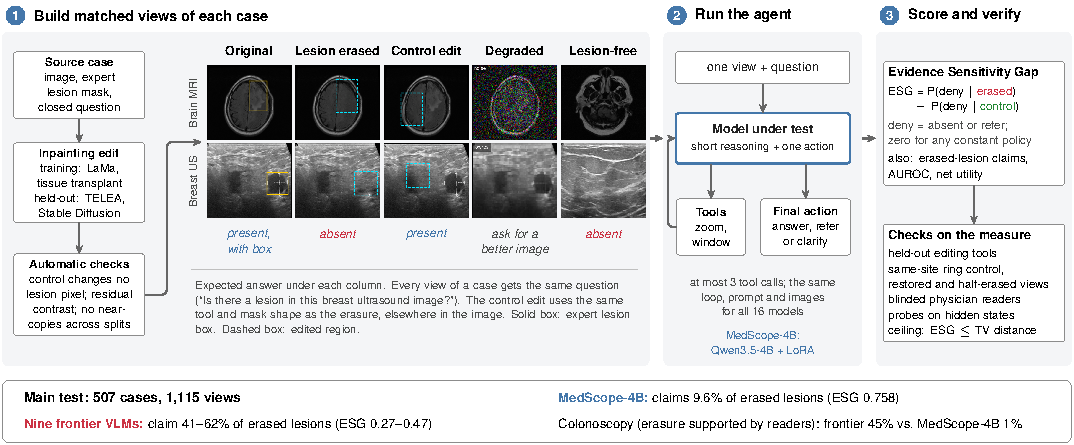
\includegraphics[width=\textwidth]{figures/fig1_framework.pdf}
\end{center}
\vspace{-0.3cm}
\caption{The Counterfactual Evidence Framework, shown on two real cases from the public data (brain MRI, TCGA-LGG; breast ultrasound, BUSI). (1) Each source case with an expert lesion mask yields matched views, all asked the same closed question: the original; the erasure ($E$, dilated mask inpainted); a control edit of the same shape and tool elsewhere ($C_{\text{far}}$); degraded views; and unedited lesion-free images, with the expected action under each column. Training uses LaMa and tissue-transplant edits; TELEA and Stable Diffusion are held out. Stage~0 adds the same-site ring control ($C_{\text{ring}}$, an area-matched ring 2\,px outside the lesion) and restored and half-erased views (not drawn). (2) Every model, frontier, open or trained, runs the same agent loop with the same prompt, tools and images. (3) What the framework reports and the checks on the measure. The bottom strip gives the main-test headline numbers (Table~\ref{tab:main_results}).}
\label{fig:framework_overview}
\vspace{-0.2cm}
\end{figure*}

\subsection{Counterfactual Views and Symmetric Controls}
\label{subsec:method_views}
We construct counterfactual episodes from public medical segmentation datasets where each case consists of an image $I$ of height $h$ and width $w$, an expert binary lesion mask $M$ (excluding lesions smaller than $20\text{ px}$ or exceeding $20\%$ of the image area), and a clinical question $Q$ whose ground-truth answer depends on the presence of the segmented lesion. To isolate visual evidence while controlling for editing artifacts and anatomical location, we construct five core view types per case:
\begin{enumerate}[leftmargin=*,nosep]
    \item \textbf{Original ($O$):} The unmodified image $I$. Expected action: correct positive answer with a bounding box localizing the lesion.
    \item \textbf{Target removal ($E$):} The lesion mask $M$ is morphologically dilated by $5\text{ px}$ ($M_{\text{dil}}$) and inpainted using LaMa \citep{suvorov2022lama}. Expected action: explicit absent answer (\emph{``No''} to \emph{``Is there\dots?''}, \emph{``Yes''} to \emph{``Is \dots\ healthy?''}, or \emph{``No abnormality''} to open queries).
    \item \textbf{Random-removal control ($C_{\text{far}}$):} The identical dilated mask shape $M_{\text{dil}}$ is translated to a random foreground tissue location that does not intersect $M_{\text{dil}}$ and is inpainted with the exact same tool. No pixel within the true lesion $M$ is altered. Expected action: the original positive answer and lesion bounding box.
    \item \textbf{Degraded view ($D$):} The image is corrupted via Gaussian blur ($\sigma = \max(h,w)/40$), additive Gaussian noise ($\sigma = 60$), $8\times$ down/up-sampling, severe JPEG compression, motion blur, or substitution with an image of a different anatomical modality. Expected action: \texttt{clarify}.
    \item \textbf{Natural negative ($N$):} An unedited lesion-free image from the same modality and source, assigned the exact same reward structure as target removal $E$. Including $N$ ensures that a shortcut policy that simply answers \emph{``absent''} whenever it detects an inpainting artifact cannot succeed on unedited healthy images.
\end{enumerate}

\textbf{Training-only views and held-out editing tools.} During training, we additionally construct \emph{lesion-insertion} views (copying a real segmented lesion into a healthy training image) and apply a second erasure mechanism---\emph{tissue transplant} (Poisson-blended healthy tissue from the same image)---to half of the training cases. To test whether evidence sensitivity transfers to unseen editing mechanisms, test-set target removals and random-removal controls are regenerated on the exact same masks using two held-out inpainting tools never seen in training: classical partial differential equation inpainting (\textbf{TELEA} \citep{telea2004image}) and \textbf{Stable Diffusion} inpainting \citep{rombach2022high}. We also evaluate a Stage-1 \emph{tool-family} training variant in which each training case's erasure and control edit are generated with one tool sampled from $\{\text{LaMa}, \text{blur fill}, \text{mean fill with noise}, \text{shuffled pixels}\}$.

\textbf{Same-site ring controls and graded evidence.} Because $C_{\text{far}}$ edits tissue away from the lesion while $E$ edits at the lesion, a model could theoretically learn a location-conditioned shortcut (\emph{``edited at the queried anatomical site means absent''}). To test this directly, we introduce three site-matched views in Stage 0 of our framework: (i) the \textbf{Same-Site Ring Control ($C_{\text{ring}}$)}, where the inpainting tool fills an area-matched ring starting $2\text{ px}$ outside the lesion boundary while leaving all lesion pixels intact; (ii) the \textbf{Restored view ($R$)}, formed by taking the erased view $E$ and restoring the lesion's original pixels; and (iii) the \textbf{Partial erasure ($P$)}, where exactly half of the lesion mask is erased with LaMa to provide graded visual evidence.

\textbf{Automated quality control.} All edited views pass through a strict, automated quality control pipeline without human intervention: (1) the erased region's contrast against a surrounding $6\text{--}14\text{ px}$ ring must be $\le \max(1.0, 0.35 \times \text{contrast}_{\text{before}})$, and a trained edit detector must score the region below $0.5$; (2) zero lesion pixels may change in $C_{\text{far}}$; (3) near-duplicate images across splits are prevented via $64$-bit difference hashing and pixel correlation across all $6,849$ unedited images; and (4) views undergo adversarial filtering until a texture classifier separates target from random edits at $\text{AUC} \le 0.60$ ($0.56$ on the main test set; a hand-crafted shortcut classifier on training views reached $\text{AUC } 0.59$).

\subsection{Evidence Sensitivity Metrics, Cost Matrix, and Abstention Ceiling}
\label{subsec:method_metrics}
Let a model or decision policy $\pi$ map a view and question $(V, Q)$ to a terminal action $a \in \{\text{claim}, \text{absent}, \text{refer}, \text{clarify}\}$. We define the primary metric, the \textbf{Evidence Sensitivity Gap (ESG)}, as the difference in denial/referral probability between target removal and the matched random-removal control:
\begin{equation}
\label{eq:esg}
\begin{split}
\text{ESG}(\pi) = {}& P\big(a \in \{\text{absent}, \text{refer}\} \mid E\big)\\
&- P\big(a \in \{\text{absent}, \text{refer}\} \mid C_{\text{far}}\big).
\end{split}
\end{equation}
By construction, $\text{ESG}(\pi) = 0$ for any constant policy (always claiming, always denying, or always referring) and, in expectation, for any policy that ignores the image or reacts identically to both edits. We also report \textbf{Strict ESG} (counting explicit $\text{absent}$ answers only) and the site-matched gap $\text{ESG}_{\text{site}} = P(a \in \{\text{absent}, \text{refer}\} \mid E) - P(a \in \{\text{absent}, \text{refer}\} \mid C_{\text{ring}})$.

Alongside ESG, we report: \textbf{Erased-lesion claims} $P(a = \text{claim} \mid E)$; \textbf{Healthy-image claims} $P(a = \text{claim} \mid N)$; \textbf{covered-and-correct rate (CCR)}, the share of answerable views ($O \cup C_{\text{far}}$) answered correctly; \textbf{Grounded accuracy}, the fraction of answerable views answered correctly with a predicted bounding box achieving $\text{IoU} \ge 0.3$ against $M$; \textbf{Area Under the Risk--Coverage Curve (AURC)} \citep{geifman2017selective} for selective prediction; and \textbf{Net Utility}, the mean reward across all views under a cost matrix fixed on 30 October 2026, after two revisions during piloting and before any model reported here was trained (Table~\ref{tab:cost_matrix}). A correct answer on $O \cup C_{\text{far}}$ with box $\text{IoU} \ge 0.3$ earns a $+0.5$ grounding bonus (boxes covering $>50\%$ of the image earn no bonus), unparseable outputs score $-1.0$, and each tool call beyond the first incurs a $-0.05$ penalty.

\begin{table*}[!t]
\caption{Cost matrix defining per-view rewards and the model selection objective (fixed before any reported model was trained; not elicited from clinicians). A miss costs $-4.0$ when the finding was flagged in advance as critical: brain tumour, malignant breast lesion, pneumothorax or mass on chest X-ray, and CT/MRI findings labelled cancer or tumour. A $+0.5$ grounding bonus is added on Original and Random-removal views when the predicted bounding box achieves $\text{IoU} \ge 0.3$ (with area $\le 50\%$ of the image).}
\label{tab:cost_matrix}
\vspace{-0.2cm}
\begin{center}
\small
\begin{adjustbox}{max width=\linewidth}
\begin{tabular}{lcccc}
\toprule
\textbf{View Type} & \textbf{Correct / Absent} & \textbf{Wrong / Claims Finding} & \textbf{Refer} & \textbf{Clarify} \\
\midrule
Original ($O$), Random removal ($C_{\text{far}}$) & $+1.0$ & $-2.0$ ($-4.0$ critical) & $-0.3$ & $-0.3$ \\
Target removal ($E$), Natural negative ($N$) & $+1.0$ & $-2.0$ & $+0.5$ & $-0.5$ \\
Degraded ($D$) & $+0.25$ & $-2.0$ & $0.0$ & $+0.5$ \\
\bottomrule
\end{tabular}
\end{adjustbox}
\end{center}
\vspace{-0.2cm}
\end{table*}

\textbf{Separating discrimination from threshold and the Abstention Ceiling.} Because ESG and Net Utility evaluate discrete decisions at a fixed operating point, we separately compute threshold-free non-parametric discrimination---$\text{AUROC}_{\text{far}}$ ($E$ vs.\ $C_{\text{far}}$) and $\text{AUROC}_{\text{site}}$ ($E$ vs.\ $C_{\text{ring}}$)---alongside raw denial rates and within-case single-turn decision log-odds shifts $\Delta s(V) = s(V) - s(O)$, where $s(x) = \log p(\text{present reply} \mid x) - \log p(\text{absent reply} \mid x)$ evaluated on identical reply tokens within each case. Furthermore, we formalize why post-hoc abstention or test-time evidence combiners cannot create evidence sensitivity beyond their inputs:

\textbf{Proposition 1 (Abstention Ceiling).} \emph{Let $S = f(V, Q)$ be any set of signals extracted from view $V$ and question $Q$ (e.g., model logits, confidence scores, or multi-agent outputs), and let $\pi: S \to \{\text{claim}, \text{absent}, \text{refer}, \text{clarify}\}$ be any deterministic or randomized decision policy operating solely on $S$. Let $D = \mathbb{I}[\pi(S) \in \{\text{absent}, \text{refer}\}]$. Then}
\begin{equation}
\label{eq:abstention_ceiling}
\begin{split}
\text{ESG}(\pi) &= P(D = 1 \mid E) - P(D = 1 \mid C_{\text{far}})\\
&\le \text{TV}\big(P(S \mid E),\, P(S \mid C_{\text{far}})\big),
\end{split}
\end{equation}
\emph{where $\text{TV}(P, Q) = \sup_{A} |P(A) - Q(A)|$ is the total-variation distance.}

\emph{Proof.} For the binary random variable $D = g(S)$, $|P(D=1 \mid E) - P(D=1 \mid C_{\text{far}})| = \text{TV}(P(D \mid E), P(D \mid C_{\text{far}}))$. By the data-processing inequality for $f$-divergences (and specifically total variation) applied to the Markov chain $V \to S \to D$, $\text{TV}(P(D \mid E), P(D \mid C_{\text{far}})) \le \text{TV}(P(S \mid E), P(S \mid C_{\text{far}}))$. $\square$

Consequently, post-hoc abstention rules on existing signals $S$ cannot raise ESG above the separation already encoded in $S$, even though they can substantially raise Net Utility by routing uncertain cases to the $+0.5$ referral reward on $E$ and $N$.

\subsection{Reference Agent (\texttt{MedScope-4B}) and Pre-Registered Methods Tested}
\label{subsec:method_agent}
\textbf{Agent protocol and architecture.} In every episode, the model receives the image (PNG, long side $\le 768\text{ px}$) and question under an identical multi-turn protocol allowing at most $3$ tool calls. At each turn, the model emits brief reasoning followed by one tagged JSON action: \texttt{zoom} (integer bounding box $[x_1, y_1, x_2, y_2] \in [0, 1000]^4$ on the original image, returning a cropped view), \texttt{window} (intensity center and width in $[0, 255]$, returning a contrast-adjusted view), \texttt{answer} (final text answer, optional evidence bounding box, and confidence), \texttt{refer} (image is usable but finding is indeterminate), or \texttt{clarify} (image is degraded/unusable or depicts the wrong anatomy).

Our reference agent, \texttt{MedScope-4B}, is built on \texttt{Qwen3.5-4B} with a frozen vision encoder and LoRA adapters ($\text{rank } 16$, $\alpha = 32$, dropout $0.05$) applied to all linear layers of the language model. Training trajectories are synthesized automatically from dataset labels alone: trajectories invoke \texttt{zoom} on a jittered box around the lesion (mandatory when the lesion covers $<2\%$ of the image), invoke \texttt{window} on $30\%$ of greyscale images, and emit the expected terminal action with concise template reasoning. Half of the training questions are rephrased using four training paraphrases, while three distinct paraphrases are held out for testing. \texttt{MedScope-4B} is trained in three stages:
\begin{itemize}[leftmargin=*,nosep]
    \item \textbf{Stage 1 (Counterfactual SFT):} Supervised fine-tuning on $16,000$ counterfactual and control views for one epoch ($3,706$ optimizer steps) at learning rate $2\times 10^{-4}$.
    \item \textbf{Stage 2 (Rejection-Sampling Fine-Tuning):} Sampling $k=4$ rollouts per view at temperature $T=1.2$, retaining the highest-reward successful trajectory (repeating hard views $\times 3$), and fine-tuning at learning rate $5\times 10^{-5}$.
    \item \textbf{Stage 3 (General-VQA Replay):} Fine-tuning on $5,000$ views mixing MedScope counterfactual trajectories with standard training-split questions from VQA-RAD \citep{lau2018vqarad}, SLAKE \citep{liu2021slake}, and PathVQA \citep{he2020pathvqa} at learning rate $5\times 10^{-5}$.
\end{itemize}
Under our pre-registered selection rule (committed 1 November 2026 before any v4 data or model existed), Stage 3 is selected over Stage 2 if validation net utility satisfies $U_3 \ge U_2 - 0.02$ and healthy-image claims satisfy $H_3 \le H_2 + 0.02$. On the $540$-case validation set ($1,473$ views), $(U, H)$ progressed from $(0.585, 13.6\%)$ in Stage 1 to $(0.610, 12.7\%)$ in Stage 2 and $(0.613, 7.7\%)$ in Stage 3; Stage 3 was thus locked as \texttt{MedScope-4B} and evaluated once on all test sets without post-hoc tuning. Earlier versions of the agent had been run on the main test (v1--v3) and the external centres (v2, v3), and the v4 recipe was registered after an audit of those results. The fresh internal and fresh external cohorts were therefore assembled as confirmatory sets on which no model had been run before \texttt{MedScope-4B} was fixed.

\textbf{Pre-registered competing methods, multi-agent verifiers, and probes.} To test whether popular post-training alignment or test-time verification techniques improve evidence discrimination beyond Stage-1 counterfactual SFT, we evaluate twelve training or system arms against matched controls, each with a criterion declared in advance (the four checks C1--C4 and eight one-seed pilots or screens):
(1) \textbf{Check C1}: matched vs.\ unmatched control edit geometry and tool;
(2) \textbf{Checks C2 \& C3}: removal-based DPO \citep{rafailov2023dpo} applied either after standard non-counterfactual SFT or on top of the counterfactual recipe;
(3) \textbf{Check C4 (Control-Matched Counterfactual Consistency, CMCC)}: a paired-view consistency objective optimizing
\begin{equation}
\label{eq:cmcc}
\begin{split}
\mathcal{L}_{\text{CMCC}} = {}& \mathcal{L}_{\text{traj}} + 0.5 \cdot \text{softplus}\big(2 - (s(C_{\text{far}}) - s(E))\big)\\
&+ 0.5 \cdot \big(s(O) - s(C_{\text{far}})\big)^2 + 0.5 \cdot \mathcal{L}_{\text{first-action}},
\end{split}
\end{equation}
tested across three seed pairs against a matched-compute replay-only control;
(4) higher adapter capacity (\textbf{LoRA rank 64}) and \textbf{Vision Encoder LoRA} at learning rates $2\times 10^{-4}$ and $2\times 10^{-5}$;
(5) \textbf{GRPO} \citep{shao2024deepseekmath} trained directly on the cost-matrix reward for $150$ steps;
(6) \textbf{Counterfactual Multi-Agent Readers (v10 and v11)} combining a direct reader, a question-blind reader, a dedicated lesion segmenter, an erase-and-re-ask counterfactual verifier, and a trained arbiter (trained in-sample in v10 and on out-of-sample reports in v11);
(7) a split-validation screening funnel of \textbf{270 decision policies} (128 Stage-A policies over stored agent/multi-agent outputs and 142 Stage-B policies incorporating test-time image augmentations, crops, token probabilities, \texttt{Qwen2.5-VL-7B}, and segmenter scores); and
(8) \textbf{Stage-1 Tool-Family training} with and without CMCC.
Finally, we conduct a \textbf{blinded two-physician reader study} ($128$ main-test views across $O, E, C_{\text{far}}, N$) and train $5$-fold case-grouped \textbf{logistic regression linear probes} \citep{alain2016understanding} on hidden states (last prompt token and mean image tokens across $8$ layers) to compare internal feature separation against behavioral output AUROC.

\textbf{Design choices.} Table~\ref{tab:design} gives the reason for each fixed choice and where its effect is checked.

\begin{table*}[!t]
\caption{Fixed design choices, why they were made, and where their effect is checked. All were fixed before \texttt{MedScope-4B} was trained; earlier versions of the agent had been run on the main test (Section~\ref{subsec:method_agent}).}
\label{tab:design}
\begin{center}
\small
\begin{adjustbox}{max width=\linewidth}
\begin{tabular}{L{2.6cm}L{3.4cm}L{4.6cm}L{3.6cm}}
\toprule
\textbf{Choice} & \textbf{Value} & \textbf{Why} & \textbf{Checked in} \\
\midrule
Base model & \texttt{Qwen3.5-4B} & Open weights; LoRA training fits one 40\,GB GPU & Recipe repeated on \texttt{MedGemma 1.5 4B} (Fig.~\ref{fig:heldout_tools_and_ablations}c) \\
Adapter & LoRA rank 16, $\alpha = 32$, language model only & Keeps the pretrained visual features; smallest adapter & Rank 64; vision adapters at two learning rates and with layer-wise decay (Secs.~\ref{subsec:exp_negative_map}, \ref{subsec:exp_review}) \\
Edit region & Lesion mask dilated by 5\,px & Removes the lesion margin as well as the annotated interior & Contrast check against a 6--14\,px ring; reader study \\
Lesion size & 20\,px to $20\%$ of the image & Smaller or larger lesions cannot be erased and checked reliably & Lesion-size quartiles (Fig.~\ref{fig:readers_robustness}b2) \\
Control edit & Same shape and tool, elsewhere, lesion untouched & Changes everything but the lesion, so ESG cancels edit effects & $2\times 2$ factorial (Fig.~\ref{fig:heldout_tools_and_ablations}b) \\
Ring control & Area-matched ring 2\,px outside the lesion & An edit at the lesion's site with the lesion intact & Stage 0 (Fig.~\ref{fig:stage0_probes}) \\
Editing tools & Training: LaMa, tissue transplant; test only: TELEA, Stable Diffusion & Tests whether sensitivity transfers to editors never seen & Fig.~\ref{fig:heldout_tools_and_ablations}a \\
Image size & Long side at most 768\,px for every model & Same input for every model & -- \\
Cost matrix & Table~\ref{tab:cost_matrix} & A missed critical finding costs most ($-4.0$), then a false claim or another miss ($-2.0$); fixed before any reported model was trained & Five alternative matrices (\ref{app:prereg_and_funnel}) \\
Stage selection & $U_3 \ge U_2 - 0.02$, $H_3 \le H_2 + 0.02$ & Fixed before v4 data existed; validation only & -- \\
Uncertainty & 2{,}000 case-bootstrap resamples, Bonferroni over 27 primary tests & Views of one case are dependent & Patient-level bootstrap (Sec.~\ref{subsec:exp_setup}) \\
\bottomrule
\end{tabular}
\end{adjustbox}
\end{center}
\end{table*}
%%%%%%%%% METHOD %%%%%%%%%

\subsection{Natural Pairs: A Real Lesion Against a Real Absence in the Same Patient}
\label{subsec:method_natural}
Every view above except the lesion-free images is made by editing, and the lesion-free images come from other patients. To test evidence sensitivity with no edit at all, we pair an unedited image that shows a lesion with an unedited image of the \emph{same patient} that does not. The pair-construction and reading rules were committed before any image or answer was seen (repository document \texttt{REVIEW\_EXPERIMENTS.md}, Amendment~4); the context-matched frames and the training rules below were added in Amendment~6, after the first natural-pair result.

\textbf{Colonoscopy (primary).} REAL-Colon \citep{biffi2024realcolon} holds $60$ full colonoscopy videos from four centres with a box on every frame in which a resected polyp is visible; no model of this project had been trained or tested on it (the dataset is public, so nothing can be said about the training data of the API models). A \emph{track} is a run of boxed frames (gaps under $2$\,s merged, at least $1$\,s long). For each of a video's three longest tracks, the lesion frame comes from the middle half of the track (largest box at least $1\%$ of the frame) and the paired frame from $10$--$30$\,s before the track starts (after it ends if fewer than three frames qualify before, as in the selection code committed with the amendment, whose prose says ``if no frame qualifies''; $28$ of the $103$ pairs take the frame after the track), at least $10$\,s from any boxed frame. Lesion-free means that no box is present; the frames were not re-read by an endoscopist. On each side the sharpest of $12$ evenly spaced candidates with mean brightness $40$--$215$ is kept. Both frames are asked \emph{``Is there a polyp in this image?''} under the agent protocol of Section~\ref{subsec:method_agent}. This gives $103$ pairs from $46$ of the $60$ videos; the number of pairs is fixed by the dataset, not by a power analysis.

\textbf{Natural ESG.} $\text{ESG}_{\text{nat}} = P(\text{absent or refer} \mid \text{lesion-free frame}) - P(\text{absent or refer} \mid \text{lesion frame})$, which is zero for any constant policy, as ESG is. Intervals and paired differences resample whole videos ($2{,}000$ resamples).

\textbf{Context-matched frames (secondary).} A frame taken $10$--$30$\,s before a polyp appears can differ from the lesion frame in more than the polyp: the endoscopist has not yet stopped to inspect. As the natural analogue of the control edit, each pair also receives a lesion-free frame from the same stretch of the examination, within $10$\,s of the track's ends and $3$--$10$\,s from the nearest boxed frame (found for $96$ of the $103$ pairs; Amendment~6).

\textbf{Chest X-ray (secondary).} Follow-up pairs from NIH ChestX-ray14 \citep{wang2017chestx}: a film whose only label is pneumothorax, effusion, nodule or mass, and the nearest ``No Finding'' film of the same patient and view position. These labels are mined from reports.

\textbf{Natural pairs in training (v5, post hoc).} A second plan, committed after the first natural-pair result (Section~\ref{subsec:exp_natural}) and before any training frame was drawn (Amendment~6), adds natural pairs to training and tests again on patients the model has never seen. From every REAL-Colon video, by rules close to the test's, we drew polyp frames from up to ten tracks (one per $2$\,s of track, at most six per track, largest box at least $0.5\%$ of the frame) and about as many lesion-free frames (near a track, context-matched, or at least $30$\,s from any polyp; a video without tracks gives twelve): $1{,}727$ polyp frames, $772$ of them with a polyp under $2\%$ of the frame, and $1{,}881$ lesion-free frames. The videos are cut into three folds by their number within each centre (videos $1$--$5$, $6$--$10$, $11$--$15$). Each model repeats the last training stage of the post hoc model v4.2 (Section~\ref{subsec:exp_review}; same data, options and seed) with natural frames added: three fold models, each trained without one fold's videos, and \texttt{v5}, trained with all $60$. Each of the $103$ pairs is answered by the fold model that never saw its video (``v5, cross-validated''); \texttt{v5} is the model run on every other test. Each model was trained once and nothing was tuned; the four trainings and all tests took about eight hours on one A100 (80\,GB).

\section{Experiments}
\label{sec:experiments}
%%%%%%%%% EXPERIMENTS %%%%%%%%%

\subsection{Datasets, Baselines, and Statistical Protocol}
\label{subsec:exp_setup}
\textbf{Datasets.} We chose sources that release expert lesion masks (needed to erase a lesion and to place a control edit of the same shape) and lesion-free images of the same imaging type, covering five imaging types with different kinds of findings (focal mucosal, mass, opacity, tumour). Training, validation, and internal main-test splits are constructed from five public sources: SLAKE \citep{liu2021slake} (CT and MRI of several body regions), Kvasir-SEG \citep{jha2020kvasir} supplemented with HyperKvasir \citep{borgli2020hyperkvasir} normal landmarks (colonoscopy), ChestX-Det \citep{liu2020chestxdet} from NIH ChestX-ray14 (chest X-ray), BUSI \citep{al2020dataset} (breast ultrasound), and TCGA-LGG \citep{buda2019association} (brain MRI FLAIR). After quality checks, training comprises $1,508$ SLAKE and colonoscopy cases plus $1,792$ chest X-ray, breast ultrasound, and brain MRI cases, alongside $427$ lesion-free HyperKvasir colonoscopy frames (normal caecum, retroflexed rectum and ileum landmarks) and $690$ lesion-free chest X-ray, breast ultrasound and brain MRI images. Excluded before splitting were $179$ of $642$ SLAKE masks (grey levels not listed in the mask key), $623$ diffuse chest X-ray findings and $179$ lesions outside the size limits in ChestX-Det, $88$ BUSI lesions too large to erase, and $364$ TCGA-LGG slices with little brain. Validation contains $540$ cases ($1,473$ views). The internal \textbf{main test set} contains $507$ cases ($219$ with expert lesion masks and $288$ lesion-free natural negatives), yielding $1,115$ total views ($219$ original, $219$ target removal, $219$ random removal, $170$ degraded, and $288$ natural negatives), split strictly by patient ID (ChestX-Det, TCGA-LGG) or near-copy perceptual groups (SLAKE, Kvasir-SEG, BUSI).

To evaluate out-of-distribution generalization and prevent overfitting, we test on six additional cohorts (summarized in Table~\ref{tab:datasets_overview}; REAL-Colon and follow-up studies from NIH ChestX-ray14 are used only for the natural pairs of Section~\ref{subsec:method_natural}): \textbf{External centres} ($169$ cases from CVC-ClinicDB, QaTa-COV19, BUS-BRA, and BraTS-Africa 2023), \textbf{Fresh internal} ($76$ unused ChestX-Det patients), \textbf{Fresh external} ($316$ cases from BraTS 2023 meningioma, BUS-UCLM, SIIM-ACR pneumothorax, and ETIS-LaribPolypDB), \textbf{Held-out wordings} ($373$ main-test cases with three unseen question paraphrases), \textbf{Standard VQA} ($1,051$ test items from VQA-RAD \citep{lau2018vqarad}, SLAKE English \citep{liu2021slake}, and PathVQA \citep{he2020pathvqa}), and \textbf{Held-out editing tools} ($125$ and $219$ main-test cases remade with unseen TELEA \citep{telea2004image} and Stable Diffusion \citep{rombach2022high} inpainting). A $64$-bit difference-hash audit across all $6,849$ unedited images confirmed that exactly one image recurred across splits (a lesion-free ChestX-Det validation image matching one SIIM fresh-external case; excluding it alters fresh-external ESG by $+0.002$, CCR by $+0.003$, and net utility by $+0.007$).

\textbf{Data leakage and patient-level splits.} Every image is assigned to its split before any view is built: all counterfactual, control, degraded and paraphrased views of an image, and every lesion insertion (made only from training images), stay in that image's split. Every fitted quantity uses training or validation data only: the stage-3 selection rule, the 270 decision policies (split-half on validation), the probes (cross-validated by case) and the review checks (Section~\ref{subsec:exp_review}). Splits are made per patient where the source releases patient identifiers (ChestX-Det via NIH ChestX-ray14, TCGA-LGG) and otherwise per group of near-identical images (SLAKE, Kvasir-SEG with HyperKvasir, BUSI), because these sources release no patient identifiers; for them, two images of one patient that are not near-copies can fall into different splits, and we cannot rule this out (a worst-case exclusion is in Section~\ref{subsec:exp_review}). Every patient holding an existing test image was removed from all v4 training and validation splits, and the fresh internal test uses only unused test-split patients. A cross-set audit hashed every unedited image of every split and cohort ($5{,}257$ training, $540$ validation, $491$ main-test, $169$ external, $76$ fresh internal and $316$ fresh external images): no case, patient or group identifier is shared by any two sets, and exactly one image recurs (the ChestX-Det validation image noted above). Pairs that are similar but not identical stay within the similarity range of images that cannot share a patient. The main test holds $507$ cases from $416$ patients or groups ($39$ groups with more than one case, at most $8$); the external centres $169$ cases from $155$, the fresh internal set $76$ from $75$ and the fresh external set $316$ from $230$. Resampling whole patients or groups instead of cases widens the intervals by at most $0.01$ (main test) and $0.03$ (fresh external); all $27$ primary comparisons stay significant, and one secondary comparison crosses $0.05$ (fresh-external ESG vs.\ \texttt{Claude Opus 5.5}, $p = 0.037 \to 0.060$).

\begin{table*}[!t]
\caption{Summary of the internal main test set (top) and the six external, confirmatory, and stress-test evaluation cohorts (bottom). $^{\dagger}$Lesion-free images built for the fresh external set; $316$ cases were evaluated in total.}
\label{tab:datasets_overview}
\vspace{-0.2cm}
\begin{center}
\small
\begin{adjustbox}{max width=\linewidth}
\begin{tabular}{llccc}
\toprule
\textbf{Cohort / Source} & \textbf{Imaging Modality or Composition} & \textbf{Masked} & \textbf{Lesion-Free} & \textbf{Total Cases (Views)} \\
\midrule
SLAKE & CT / MRI (near-copy split) & 17 & 90 & 107 \\
Kvasir-SEG + HyperKvasir & Colonoscopy (near-copy split) & 83 & 91 & 174 \\
ChestX-Det & Chest X-ray (patient split) & 41 & 50 & 91 \\
BUSI & Breast ultrasound (near-copy split) & 42 & 15 & 57 \\
TCGA-LGG & Brain MRI FLAIR (patient split) & 36 & 42 & 78 \\
\textbf{Main Test Total} & \textbf{5 modalities (170 degraded views)} & \textbf{219} & \textbf{288} & \textbf{507 (1,115)} \\
\midrule
External centres & CVC-ClinicDB (40), QaTa-COV19 (20), & 119 & 50 & 169 \\
 & BUS-BRA (45), BraTS-Africa 2023 (64) & & & \\
Fresh internal & Unused ChestX-Det test patients & 36 & 40 & 76 \\
Fresh external & BraTS meningioma (82), BUS-UCLM (99), & 168 & 150$^{\dagger}$ & 316 \\
 & SIIM pneumothorax (96), ETIS-Larib (39) & & & \\
Held-out wordings & Main test with 3 test-only paraphrases & -- & -- & 373 \\
Standard VQA & VQA-RAD (451), SLAKE (300), PathVQA (300) & -- & -- & 1,051 \\
Held-out editing tools & TELEA, Stable Diffusion, Transplant & 125 / 219 & -- & 125 / 219 \\
\bottomrule
\end{tabular}
\end{adjustbox}
\end{center}
\vspace{-0.2cm}
\end{table*}

\textbf{Baselines and statistical protocol.} We compare \texttt{MedScope-4B} against nine frontier VLMs evaluated via their public APIs under provider default settings on 31 October 2026 (OpenAI \texttt{gpt-6-sol}, \texttt{gpt-6-astra}, \texttt{gpt-6.1-sol}; Anthropic \texttt{Claude Fable 5.1}, \texttt{Claude Opus 5.5}, \texttt{Claude Sonnet 5.5}; and Google \texttt{gemini-4-argon}, \texttt{gemini-3.1-pro-preview}, and \texttt{gemini-3.8-flash}), six open-weight VLMs run locally in \texttt{bfloat16} with greedy decoding (\texttt{Qwen3.5-4B} base, \texttt{MedGemma 1.5 4B}, \texttt{Lingshu-7B}, \texttt{HuatuoGPT-Vision-7B}, \texttt{Qwen2.5-VL-7B}, and \texttt{Qwen3-VL-8B}), and three trivial constant policies (the per-view transcripts and judged outputs of every run are released with MedScope-Bench on Hugging Face). All $95\%$ confidence intervals are computed via $2,000$ case-clustered bootstrap resamples (resampling all views of a case together; resampling whole patients or near-copy groups widens intervals by $\le 0.01$ on the main test and $\le 0.03$ on fresh external). Two-tailed paired bootstrap $p$-values across the $27$ primary comparisons (ESG, erased-lesion claims, and net utility against the nine frontier models) are evaluated against a Bonferroni-corrected threshold of $\alpha = 0.05/27$. Each training stage used one NVIDIA A100 40 GB GPU for about $4\text{ h}$ (later pilots used an A100 80 GB and an RTX PRO 6000 96 GB) (PyTorch 2.11, Transformers 5.22.1, PEFT 0.21.2); frontier API runs on the main test cost US\$132, and the 48 API runs up to the preprint cost US\$373 in total (the later natural-pair, context-frame and open-ended runs are not included in this figure).

\subsection{Main Benchmark Results and Frontier Model Robustness}
\label{subsec:exp_main}
Table~\ref{tab:main_results} and Figure~\ref{fig:frontier_vs_medscope_main}a present the main benchmark results across all $507$ cases ($1,115$ views). While all nine frontier VLMs achieve high answerable accuracy ($\text{CCR } 0.829\text{--}0.888$), they claim the queried lesion on $41.1\%$ (\texttt{gemini-4-argon}) to $61.6\%$ (\texttt{gemini-3.8-flash}) of target-erased views, with ESG between $0.269$ and $0.470$. In contrast, \texttt{MedScope-4B} achieves an ESG of $0.758$ $[0.701, 0.815]$, reduces erased-lesion claims to $9.6\%$ $[6.1, 13.7]$ and healthy-image claims to $7.6\%$ $[4.8, 10.9]$, maintains a competitive CCR of $0.849$, and reaches a Net Utility of $0.732$ $[0.649, 0.813]$. Furthermore, \texttt{MedScope-4B} correctly asks to \texttt{clarify} on all $170/170$ degraded views. Two checks show that neither referral nor the degraded views carry the comparison: counting explicit ``absent'' answers only (Strict ESG) gives $0.758$ for \texttt{MedScope-4B} and $0.237$--$0.470$ for the nine frontier models, and without the degraded views net utility is $0.774$ against $0.310$, $0.361$ and $0.579$ for \texttt{gpt-6-astra}, \texttt{Claude Opus 5.5} and \texttt{gemini-4-argon} (each $p < 0.001$). \texttt{MedScope-4B}'s grounded accuracy is $0.785$.

\begin{table*}[!t]
\caption{Main test performance across $507$ cases ($1,115$ views) under the identical multi-turn agent protocol. Erased \% denotes false finding claims on $219$ target-erased views; Healthy \% denotes false claims on $288$ unedited lesion-free views; CCR is measured over $438$ answerable views ($O \cup C_{\text{far}}$). Bracketed ranges for \texttt{MedScope-4B} indicate $95\%$ case-clustered bootstrap confidence intervals.}
\label{tab:main_results}
\vspace{-0.2cm}
\begin{center}
\small
\begin{adjustbox}{max width=\linewidth}
\begin{tabular}{lccccc}
\toprule
\textbf{Model} & \textbf{CCR} $\uparrow$ & \textbf{ESG} $\uparrow$ & \textbf{Erased \%} $\downarrow$ & \textbf{Healthy \%} $\downarrow$ & \textbf{Net Utility} $\uparrow$ \\
\midrule
\textbf{MedScope-4B (Ours)} & 0.849 & \textbf{0.758} [0.701, 0.815] & \textbf{9.6} [6.1, 13.7] & \textbf{7.6} [4.8, 10.9] & \textbf{0.732} [0.649, 0.813] \\
\midrule
gemini-4-argon & 0.874 & 0.470 & 41.1 & 9.0 & 0.565 \\
Claude Sonnet 5.5 & 0.870 & 0.402 & 48.4 & 16.7 & 0.381 \\
gemini-3.1-pro-preview & 0.849 & 0.384 & 51.6 & 26.7 & 0.306 \\
gpt-6-sol & 0.829 & 0.342 & 51.6 & 25.7 & 0.261 \\
Claude Fable 5.1 & 0.856 & 0.342 & 52.1 & 23.3 & 0.255 \\
Claude Opus 5.5 & 0.863 & 0.329 & 53.9 & 23.6 & 0.358 \\
gpt-6.1-sol & \textbf{0.888} & 0.324 & 58.9 & 30.9 & 0.276 \\
gpt-6-astra & 0.886 & 0.306 & 58.9 & 27.8 & 0.309 \\
gemini-3.8-flash & 0.868 & 0.269 & 61.6 & 27.8 & 0.263 \\
\midrule
Lingshu-7B & 0.527 & 0.416 & 32.0 & 12.5 & $-0.249$ \\
Qwen3.5-4B (base) & 0.758 & 0.338 & 42.0 & 19.4 & 0.134 \\
Qwen3-VL-8B & 0.553 & 0.297 & 12.8 & 12.5 & 0.186 \\
MedGemma 1.5 4B & 0.674 & 0.283 & 54.3 & 24.0 & $-0.255$ \\
HuatuoGPT-Vision-7B & 0.498 & 0.265 & 30.1 & 22.9 & $-0.426$ \\
Qwen2.5-VL-7B & 0.144 & 0.146 & 5.5 & 24.7 & $-0.742$ \\
\midrule
Always claims finding & 1.000 & 0.000 & 100.0 & 100.0 & $-0.478$ \\
Always says absent & 0.000 & 0.000 & 0.0 & 0.0 & $-0.848$ \\
Always refers & 0.000 & 0.000 & 0.0 & 0.0 & 0.110 \\
\bottomrule
\end{tabular}
\end{adjustbox}
\end{center}
\vspace{-0.2cm}
\end{table*}

\begin{figure*}[!t]
\begin{center}
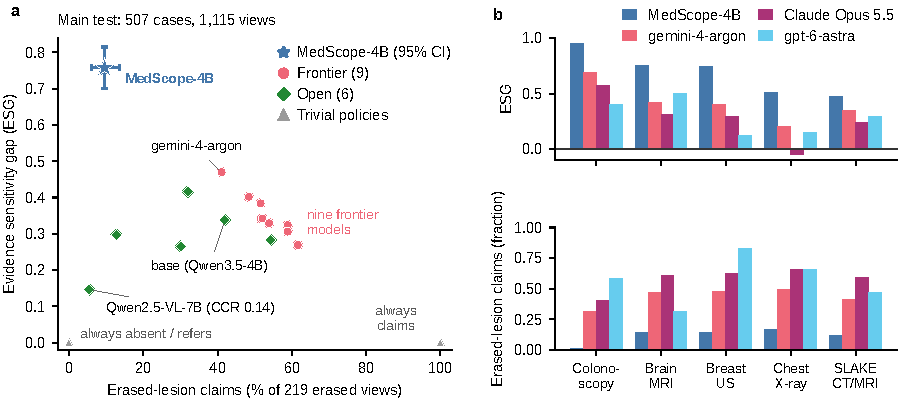
\includegraphics[width=\textwidth]{figures/fig2_main_test.pdf}
\end{center}
\vspace{-0.3cm}
\caption{Frontier VLMs claim $41$--$62\%$ of erased findings; \texttt{MedScope-4B} claims $9.6\%$, on every imaging type. Main test ($507$ cases, $1{,}115$ views). (a) ESG against the share of the $219$ erased views on which each model claims the finding: \texttt{MedScope-4B} (bars: $95\%$ bootstrap intervals), the nine frontier VLMs, the six open VLMs and the trivial policies (ESG $0$). Lower claims alone are not better: \texttt{Qwen2.5-VL-7B} claims least among the open models ($5.5\%$) but answers almost nothing correctly (CCR $0.144$, ESG $0.146$). (b) By imaging type, \texttt{MedScope-4B} against the three flagships: ESG (top) and erased-lesion claims as a fraction (bottom); values in Appendix Table~\ref{tab:modality_breakdown}.}
\label{fig:frontier_vs_medscope_main}
\vspace{-0.2cm}
\end{figure*}

In paired bootstrap comparisons against each of the nine frontier models, \texttt{MedScope-4B} improves ESG by $+0.288$ to $+0.489$ (vs.\ \texttt{gemini-4-argon}: $+0.288$ $[0.208, 0.367]$, all $p < 0.001$), lowers erased-lesion claims by $-0.315$ to $-0.521$ (all $p < 0.001$), and increases Net Utility by $+0.168$ to $+0.477$ (all $p \le 0.001$), surviving Bonferroni correction across all $27$ primary tests. CCR differences between \texttt{MedScope-4B} and the frontier models range from $-0.039$ to $+0.021$ ($p \ge 0.12$; confidence intervals reach $-0.09$, so formal equivalence is not established), and healthy-image claims are significantly lower than eight of nine frontier models ($p \le 0.001$; vs.\ \texttt{gemini-4-argon} $-0.014$, $p = 0.59$). Relative to its untrained \texttt{Qwen3.5-4B} base model, \texttt{MedScope-4B} improves ESG by $+0.420$ $[0.338, 0.498]$ (and by $+0.475$ over untrained \texttt{MedGemma 1.5 4B}). Table~\ref{tab:main_results} illustrates why erased-lesion claims cannot be evaluated without matched controls: ranking models by erased claims alone produces a \textbf{ranking reversal} that prefers \texttt{Qwen2.5-VL-7B} ($5.5\%$ erased claims) over \texttt{MedScope-4B} ($9.6\%$), even though \texttt{Qwen2.5-VL-7B} achieves this solely by defaulting to \emph{``absent''} on nearly all inputs ($\text{CCR } 0.144$, $\text{ESG } 0.146$, Net Utility $-0.742$).

As shown in Figure~\ref{fig:frontier_vs_medscope_main}b (and Appendix Table~\ref{tab:modality_breakdown}), \texttt{MedScope-4B} is ahead of the frontier flagships on ESG and erased-lesion claims in all five imaging types (and on net utility in four: on SLAKE CT/MRI it has $0.22$ against $0.38$ for \texttt{gemini-4-argon} and $0.32$ for \texttt{Claude Opus 5.5}), achieving an ESG / erased-claim fraction / net utility of $0.95 / 0.01 / 1.06$ on Colonoscopy (vs.\ $0.40\text{--}0.69$ ESG and $0.31\text{--}0.58$ erased claims for flagships), $0.75 / 0.14 / 0.75$ on Brain MRI, $0.74 / 0.14 / 0.78$ on Breast Ultrasound, $0.51 / 0.17 / 0.40$ on Chest X-ray (where \texttt{Claude Opus 5.5} drops to $-0.05$ ESG), and $0.47 / 0.12 / 0.22$ on SLAKE CT/MRI.

\textbf{Prompting, reasoning, tool-use, and lesion-size robustness.} To test whether frontier false claims stem from prompt phrasing or sub-optimal inference settings, we re-evaluated \texttt{gemini-4-argon}, \texttt{Claude Opus 5.5}, and \texttt{gpt-6-astra} on a $150$-case subset across six regimes: Default, Cautious prompt, Solved in-context examples, Highest reasoning budget, Highest image resolution setting, and a Plain free-text prompt without tools (Figure~\ref{fig:readers_robustness}b1 and Appendix Table~\ref{tab:robustness_prompts}). Across all six conditions, frontier models continue to claim $36.8\%$ to $66.2\%$ of erased lesions ($\text{ESG } 0.250\text{--}0.500$), whereas \texttt{MedScope-4B} achieves $0.750$ ESG and $7.4\%$ erased claims (ahead of each flagship on ESG and net utility in every condition, with $p \le 0.012$ in every logged test). Removing the $26$ of $288$ lesion-free cases whose label a consensus of frontier models disputed leaves the comparison unchanged. Furthermore, \texttt{MedScope-4B} is unchanged on held-out question wordings ($373$ cases; net utility change $+0.006$ $[-0.033, 0.041]$) and ranks first under all five alternative clinical cost matrices tested. Refusing tool calls (\texttt{zoom} and \texttt{window}) at test time leaves \texttt{MedScope-4B} ESG unchanged ($0.753$ vs.\ $0.758$, $p = 0.92$) while reducing net utility by $0.092$ ($p = 0.003$) and CCR by $0.053$: the tools add accuracy on real lesions rather than evidence sensitivity. Stratified by lesion-area quartiles (Figure~\ref{fig:readers_robustness}b2), \texttt{MedScope-4B} ESG scales monotonically from $0.545$ in Q1 ($18.2\%$ erased claims on the smallest lesions) to $0.741$ (Q2), $0.836$ (Q3), and $0.909$ in Q4 ($1.8\%$ erased claims), whereas the three flagships stay within ESG $0.20\text{--}0.56$ in every quartile. Selective prediction is weaker: \texttt{MedScope-4B}'s verbalized confidence (emitted via short template reasoning) ranks errors less effectively than frontier models, yielding a higher AURC of $0.065$ vs.\ $0.020\text{--}0.033$.

\subsection{Active Ingredients of Counterfactual Training and Held-Out Editing Tools}
\label{subsec:exp_ablations_tools}
To isolate what drives \texttt{MedScope-4B}'s evidence sensitivity, we conduct Stage-1 training ablations (Figure~\ref{fig:heldout_tools_and_ablations}c and Appendix Table~\ref{tab:ablations_and_factorial}A), a $2\times 2$ factorial decomposition of training views (Figure~\ref{fig:heldout_tools_and_ablations}b and Appendix Table~\ref{tab:ablations_and_factorial}B), and transfer evaluations on unseen inpainting tools (Figure~\ref{fig:heldout_tools_and_ablations}a and Appendix Table~\ref{tab:heldout_tools}).

\begin{figure*}[!t]
\begin{center}
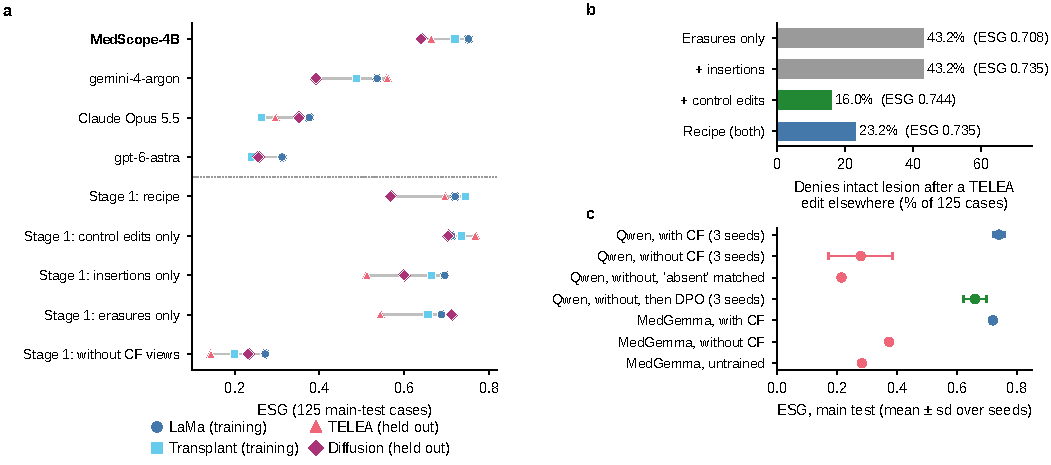
\includegraphics[width=\textwidth]{figures/fig3_tools_ablations.pdf}
\end{center}
\vspace{-0.3cm}
\caption{\texttt{MedScope-4B} leads every flagship on every editing tool, and the control edit, not lesion insertion, removes the ``edited means absent'' shortcut. (a) ESG on $125$ main-test cases whose erasures and control edits were remade with each tool on the same masks: two training tools (LaMa, tissue transplant) and two held-out tools (TELEA, Stable Diffusion). (b) $2\times 2$ factorial of training-only components (Stage~1, seed~0): share of $125$ intact lesions denied after a TELEA edit elsewhere in the image, with main-test ESG in brackets; control edits, not lesion insertions, remove the ``edited means absent'' shortcut. (c) Main-test ESG of Stage-1 arms (mean $\pm$ sd over three seeds where marked): blue, with counterfactual (CF) views; vermilion, without; green, without CF views followed by removal-based DPO (check C2); the MedGemma rows replicate the recipe on a second architecture.}
\label{fig:heldout_tools_and_ablations}
\vspace{-0.2cm}
\end{figure*}

\textbf{Counterfactual views vs.\ label priors.} Removing counterfactual views from Stage-1 SFT causes ESG to collapse from $0.741 \pm 0.019$ to $0.279 \pm 0.107$ across three seeds (per-seed differences $+0.525, +0.539, +0.324$, all $p < 0.001$; external centres ESG $0.622 \pm 0.030$ vs.\ $0.389 \pm 0.043$) and increases erased-lesion claims from $13.2\%$ to $67.6\%$ (Appendix Table~\ref{tab:ablations_and_factorial}A). To verify that this gain is not merely an artifact of exposing the model to more negative (\emph{``absent''}) labels during training, we trained an arm without counterfactual views but matched the exact proportion of \emph{``absent''} answers using natural lesion-free images; this arm achieved only $0.215$ ESG ($73.5\%$ erased claims; paired difference $+0.521$ $[0.440, 0.600]$). Replicating the Stage-1 recipe on a medical-specialized architecture, \texttt{MedGemma 1.5 4B}, similarly boosts ESG from $0.283$ (untrained) and $0.374$ (SFT without counterfactuals) to $0.721$ ($+0.347$ $[0.276, 0.425]$). Stages 2 and 3 provide modest polishing over Stage 1 on the main test (net utility $+0.040$, $p = 0.15$; ESG $+0.023$, $p = 0.39$) while halving healthy-image claims on validation ($13.6\% \to 7.7\%$).

\textbf{How control edits suppress the ``edited means absent'' shortcut.} In the $2\times 2$ factorial ablation (Figure~\ref{fig:heldout_tools_and_ablations}b and Appendix Table~\ref{tab:ablations_and_factorial}B), training on target erasures alone achieves strong main-test ESG ($0.708$) and low erased claims ($6.8\%$). However, when evaluated on $125$ cases where an unseen tool (TELEA) performs a control edit elsewhere on the image while leaving the lesion intact, the erasures-only model falsely denies $43.2\%$ of intact lesions---having learned the shortcut that \emph{any inpainted image has no lesion}. Including random-location control edits during training cuts this false denial rate to $16.0\%$ (control edits only) and $23.2\%$ (full recipe).

\textbf{Transfer to held-out editing tools and edit visibility.} Across the $125$-case multi-tool benchmark (Figure~\ref{fig:heldout_tools_and_ablations}a and Appendix Table~\ref{tab:heldout_tools}A), \texttt{MedScope-4B} keeps its evidence sensitivity on both seen tools (LaMa $0.752$, Transplant $0.720$) and unseen held-out tools (TELEA $0.664$, Stable Diffusion $0.640$), outperforming every frontier flagship on every tool ($\Delta\text{ESG } +0.10$ to $+0.48$, all $p \le 0.049$, uncorrected). \texttt{gemini-4-argon}'s erased claims drop from $32.8\%$ on LaMa to $8.8\%$ on TELEA, possibly because TELEA's smooth fills read as edits. Auditing edit visibility directly, a supervised ResNet-18 separates $C_{\text{far}}$ from $O$ at $\text{AUC } 0.83$ $[0.80, 0.87]$, and a linear probe on the frozen vision encoder's pooled features separates them at $\text{AUC } 0.60$ $[0.58, 0.63]$ (while separating $E$ from $C_{\text{far}}$ at $0.86$ $[0.83, 0.89]$). Zero-shot, however, \texttt{gemini-4-argon} and \texttt{gpt-6.1-sol} separate $C_{\text{far}}$ from $O$ near chance ($\text{AUC } 0.52\text{--}0.55$, while separating $E$ from $O$ at $0.70\text{--}0.75$). On the $61/219$ erasures that \texttt{gemini-4-argon} explicitly rates as unedited, \texttt{MedScope-4B} claims the lesion in only $15\%$ of cases ($8\%$ on visibly edited ones) compared to $41\%\text{--}64\%$ for the nine frontier models.

Examining where held-out ESG is lost across all $219$ cases for the Stage-1 recipe (Appendix Table~\ref{tab:heldout_tools}B) reveals distinct failure modes by generator: on LaMa, false control denial when the unedited lesion was found is only $2.7\%$ ($5/186$), so the remaining ESG gap comes from \emph{perception} ($33/219$ real lesions missed on $O$); on TELEA, loss is driven by \emph{edit-induced denial} of intact lesions ($12.9\%$, $24/186$, including $13$ breast ultrasound cases); and on Stable Diffusion, $41/45$ false claims on $E$ point their bounding boxes at the erased site. Diffusion erasures were not reader-checked, so these sites may hold residual or regenerated lesion-like tissue; we cannot tell which.

\subsection{Pre-Registered Negative Map: Threshold Shifts vs.\ Discrimination}
\label{subsec:exp_negative_map}
A central question of our study is whether post-training alignment, consistency losses, multi-agent verification, or test-time decision policies can push evidence discrimination beyond counterfactual SFT. Figure~\ref{fig:threshold_vs_discrimination_map} and Appendix Table~\ref{tab:negative_map_summary} synthesize our pre-registered checks (C1--C4), post-preprint training pilots, tool-family training, and the 270-policy screening funnel (numeric breakdowns in Appendix Tables~\ref{tab:negative_map_summary}, \ref{tab:app_c1_c3}, \ref{tab:app_c4_cmcc}, and \ref{tab:app_tool_family}).

\begin{figure*}[!t]
\begin{center}
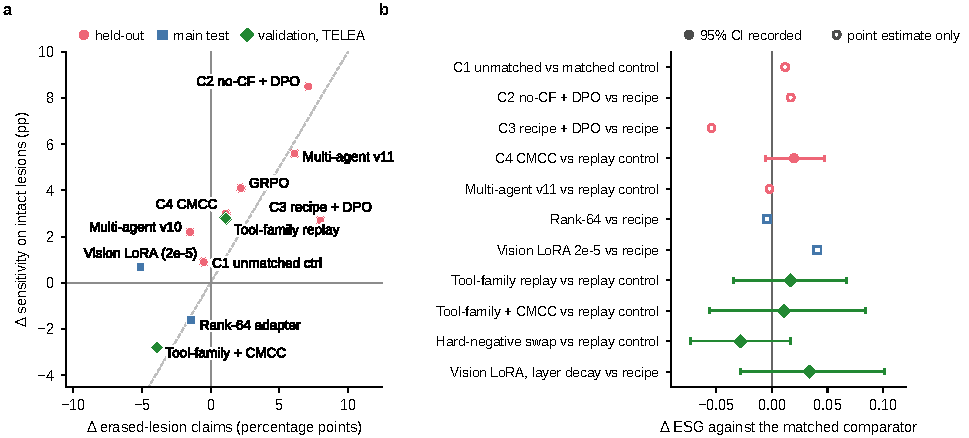
\includegraphics[width=\textwidth]{figures/fig4_negative_map.pdf}
\end{center}
\vspace{-0.3cm}
\caption{No change of objective, capacity or system shows a reliable gain over its comparator in separating erased from intact lesions: the operating point moves. (a) Each trained or system arm against its matched comparator: change in erased-lesion claims (x) and in sensitivity on intact lesions (y), in percentage points. Arms that claim more also find more, so the points follow the diagonal: the operating point moves. Held-out tools are TELEA and Stable Diffusion pooled ($219$ cases); tool-family arms are on validation TELEA views; rank-64 and vision-LoRA arms on the main test. C4 CMCC and tool-family replay nearly coincide. (b) Change in ESG for every arm with a recorded ESG difference (filled: $95\%$ interval recorded; open: point estimate only). Every recorded interval includes zero, and the point estimates lie between $-0.054$ and $+0.041$ (C3, at $-0.054$, has no recorded interval; its decrease has $p = 0.027$). GRPO and multi-agent v10 have no recorded ESG difference on these sets and appear only in A. The last two rows of B are the checks added after the review (Section~\ref{subsec:exp_review}). Values in Appendix Tables~\ref{tab:negative_map_summary}--\ref{tab:app_tool_family}.}
\label{fig:threshold_vs_discrimination_map}
\vspace{-0.2cm}
\end{figure*}

\begin{figure*}[!t]
\begin{center}
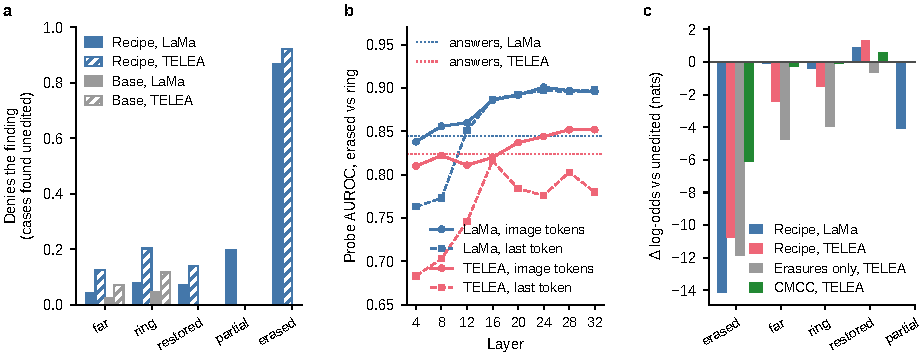
\includegraphics[width=\textwidth]{figures/fig5_stage0_probes.pdf}
\end{center}
\vspace{-0.3cm}
\caption{Denials follow the evidence rather than the edit's site, and the hidden states separate erased from intact lesions about as well as the answers do. Stage~0 on validation data (Stage-1 recipe, seed~0; untrained base model). (a) Share of intact lesions denied after each view, among cases whose unedited image the model answers present ($143$ recipe, $127$ base); the erased view is shown for reference. Partial erasure was built with LaMa only, and the restored and partial views for the recipe only. (b) Cross-validated AUROC of linear probes on the recipe's hidden states (erased vs.\ ring control) by layer, for the mean of the image tokens and the last prompt token; dotted lines give the AUROC of the recipe's own answers. (c) Within-case change of the single-turn log-odds relative to the unedited view (nats); this score failed its validity check as a cross-case score (Section~\ref{sec:discussion}) but is valid within a case.}
\label{fig:stage0_probes}
\vspace{-0.2cm}
\end{figure*}

Across all twelve trained or system arms (Appendix Table~\ref{tab:negative_map_summary}), no change of objective, capacity or system met its criterion for separating erased from intact lesions better than its matched comparator (Figure~\ref{fig:threshold_vs_discrimination_map}b); in most arms claims on erased lesions and sensitivity on intact lesions rose or fell together (Figure~\ref{fig:threshold_vs_discrimination_map}a), which we read as a move of the operating point:
\begin{itemize}[leftmargin=*,nosep]
    \item \textbf{Control Matching, DPO and Consistency Losses (C1--C4):} Matching the control edit's shape and tool to the erasure (C1) was inconclusive by its registered rule: against an unmatched control it was not shown to matter. The registered question of C2 was whether our recipe beats removal-based DPO applied after non-counterfactual SFT; on fresh external data no ESG difference was shown ($0.381 \pm 0.018$ vs.\ $0.355 \pm 0.015$ over three seeds; single-seed difference $+0.012$ $[-0.053, 0.077]$). DPO claims fewer erased lesions ($12.9 \pm 7.9\%$ vs.\ $20.0 \pm 4.0\%$) with lower lesion sensitivity ($0.485 \pm 0.086$ vs.\ $0.587 \pm 0.026$), and the recipe has the higher net utility ($0.070 \pm 0.008$ vs.\ $-0.069 \pm 0.078$). Applying DPO on top of the counterfactual recipe (C3) lowers held-out-tool ESG ($0.595$ vs.\ $0.649$, $p = 0.027$) and increases erased claims by $+8.0$ percentage points ($24.4\%$ vs.\ $16.3\%$). The paired-view CMCC loss (C4, Eq.~\ref{eq:cmcc}), registered after a favourable one-seed pilot on the same test sets, does not meet its primary endpoint across three seed pairs (held-out erased claims $+0.011$ $[-0.009, 0.030]$) and its main-test guard (healthy-image claims $+0.052$, $p<0.001$). Its fresh-external guard held (ESG $+0.058$, net utility $+0.146$), with erased claims ($+0.073$) and CCR ($+0.127$) both higher there: by penalizing differences between $O$ and $C_{\text{far}}$, it shifts all endpoints toward answering \emph{``present''}.
    \item \textbf{Adapter Capacity, Vision LoRA, and GRPO:} Increasing LoRA rank to $64$ induces a positive response bias on SIIM pneumothorax (claiming $25/48$ present, $21/48$ erased, and $12/48$ healthy; SIIM ESG $0.042$). Unfreezing the vision encoder with LoRA at $\text{lr } 2\times 10^{-4}$ collapses the model ($\text{ESG} = 0.000$ on every dataset, answering purely from question text: always claiming tumours/masses/``lesions'' and always denying polyps/effusions), while lowering the vision learning rate to $2\times 10^{-5}$ makes the model uniformly more conservative (fresh-external CCR drops $-0.071$ to $0.488$, $p=0.03$; pneumothorax $7/48$ vs.\ $10/48$; main-test erased claims $6.8\%$ vs.\ $11.9\%$). GRPO (150 steps on the cost-matrix reward) raises net utility on held-out tools (about $+0.056$) and on fresh external data ($+0.124$, ESG $+0.083$), but misses its pre-declared go signal on erased-lesion claims ($+0.022$ against the control on held-out tools); the main-test healthy-image guard passed ($+0.021$), while fresh-external healthy-image claims rose by $+0.054$. GRPO makes the model answer more, finding more real lesions and adding a few false claims.
    \item \textbf{Multi-Agent Verification (v10, v11) and Tool-Family Training:} In the 5-agent verification pipeline, ablations show that only the dedicated lesion segmenter contributes positively (removing it costs $-0.055$ to $-0.066$ net utility); although the erase-and-re-ask verifier withdraws $\sim 80\%$ of claims after erasing their box and keeps $\sim 95\%$ after a control edit, the direct reader rarely claims an erased lesion with a box ($20$ of $219$ erased views), leaving the verifier inactive. Version v10 collapses on external CCR ($0.513$ vs.\ $0.769$ on external centres; $0.378$ vs.\ $0.560$ on fresh external; $3/48$ on pneumothorax), while v11 achieves the highest main-test utility ($0.809$) only because its verifier uses the main test's own LaMa inpainter---on held-out tools, v11 yields $\Delta\text{ESG} = -0.002$ and increases erased claims by $+0.061$. Likewise, training Stage 1 with a family of four editing tools (Appendix Table~\ref{tab:app_tool_family}) fails to transfer to unseen TELEA ($\Delta\text{ESG} +0.017$ and $+0.011$, both non-significant).
    \item \textbf{Decision policies (270):} In our split-validation screening funnel (Appendix Table~\ref{tab:negative_map_summary} bottom), 19 of 128 Stage-A decision policies on stored outputs passed Half A, but \textbf{0 confirmed on Half B}. In Stage B, \textbf{0 of 142 policies} combining test-time image augmentations (mirror, crop, contrast), close-ups, first-token answer probabilities (which decouple the binary presence/absence token from the bounding-box coordinate tokens), \texttt{Qwen2.5-VL-7B}, and segmenter scores passed even Half A: while combiners raised TELEA net utility from $0.444$ to $0.686$ by abstaining/referring more often, ESG stayed at $0.55\text{--}0.61$ for most combiners (vs.\ $0.600$ for the recipe; the largest, $0.642$, came at a cut-off that failed elsewhere). Stage~A, which recombines stored signals, is the case Proposition~1 covers; Stage~B adds new signals, so the ceiling for the original signals does not bind it. Section~\ref{subsec:exp_review} measures a lower bound on the distance itself.
    \item \textbf{The exception: more training on the same views.} The matched-compute control of C4, which is the recipe adapter trained longer on the same control-edit data with no new objective, cut erased-lesion claims on unseen tools in two of three seeds ($-0.080$ and $-0.085$, $p<0.001$; $-0.012$, n.s.) and raised held-out ESG in one ($+0.076$, $p=0.001$; $+0.022$ and $+0.027$, n.s.), at one seed with a loss of clean-image sensitivity ($-0.049$, $p<0.001$). This comparison was an observation, not a registered test. Like the two coverage results of Section~\ref{subsec:disc_negative_map}, it points to exposure rather than objectives.
\end{itemize}

\subsection{Same-Site Ring Controls, Representation Probes, Physician Verification, and External Generalization}
\label{subsec:exp_probes_readers_failures}
\textbf{Stage-0 same-site ring controls and hidden-state linear probes.} Figure~\ref{fig:stage0_probes} and Appendix Table~\ref{tab:ring_and_probes} evaluate whether the Stage-1 recipe relies on edit-location shortcuts or suffers from an answer read-out gap on the validation cohort ($179$ lesion cases with yes/no questions and $80$ lesion-free images). On seen LaMa edits (Appendix Table~\ref{tab:ring_and_probes}A), intact-lesion denial on the $2\text{ px}$ same-site ring control ($0.077$) is statistically indistinguishable from far-control denial ($0.042$; difference $+0.035$ $[-0.021, 0.091]$), and $\text{AUROC}_{\text{site}}$ ($0.845$) matches $\text{AUROC}_{\text{far}}$ ($0.853$). On unseen TELEA edits, ring denial rises to $0.203$ vs.\ $0.126$ on far controls ($+0.077$ $[0.000, 0.154]$), meeting the pre-registered flag ($\ge 0.10$, $\ge +0.05$ over far, and $\ge +0.05$ over base). However, a post-hoc paired comparison on the $112$ cases detected unedited by both the recipe and the untrained base model reveals that the site-specific interaction---$(\text{ring} - \text{far})_{\text{recipe}} - (\text{ring} - \text{far})_{\text{base}}$---is only $+0.018$ $[-0.080, 0.116]$, with TELEA ring denials concentrated almost entirely in chest X-rays ($12/17$ vs.\ $0/33$ breast ultrasound, $2/34$ colonoscopy, $0/24$ brain MRI). Thus, counterfactual training roughly doubles general sensitivity to unfamiliar PDE artifacts wherever they occur ($12.5\%$ vs.\ $6.2\%$ on ring; $8.9\%$ vs.\ $4.5\%$ on far) rather than inducing a site-specific shortcut. Restoring the lesion pixels ($R$) returns denial to $0.070$ (LaMa) and $0.140$ (TELEA), and partial $50\%$ erasure ($P$) yields an intermediate denial rate of $0.196$ (and intermediate log-odds shift of $-4.05\text{ nats}$ vs.\ $-14.10\text{ nats}$ for full erasure; Figure~\ref{fig:stage0_probes}c).

Linear probes on hidden states (Figure~\ref{fig:stage0_probes}b and Appendix Table~\ref{tab:ring_and_probes}B) show that on held-out TELEA $E$ vs.\ $C_{\text{ring}}$, the best layer-wise probe achieves $\text{AUROC } 0.852$ (image tokens) and $0.816$ (last token) compared to the recipe's behavioral output AUROC of $0.824$---a read-out gap of $+0.028$ and $-0.008$, well below the pre-registered $0.05$ threshold. Moreover, the untrained base model's hidden states already separate $E$ from $C_{\text{ring}}$ at $\text{AUROC } 0.870$ (LaMa) and $0.831$ (TELEA). So the model's answers use about as much separation as its hidden states hold (no read-out gap), and the untrained base model's hidden states are nearly as separable as the trained model's. The probes were on the language model's hidden states, not on the vision encoder, so they do not locate the limit inside the encoder; together with the $20.1\%$ of unedited validation lesions the recipe misses on $O$, they point to perception rather than the read-out as the remaining limit.

\begin{figure*}[!t]
\begin{center}
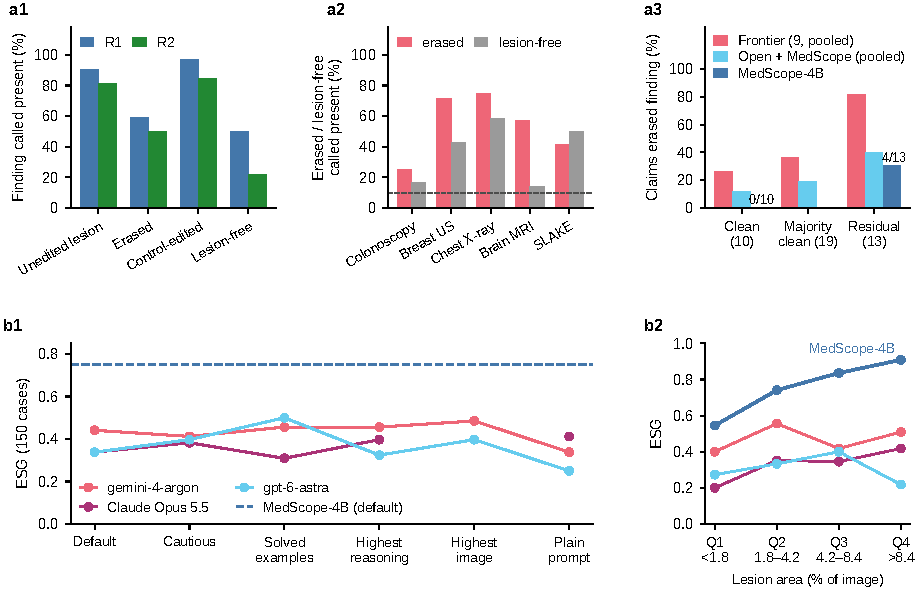
\includegraphics[width=\textwidth]{figures/fig6_readers_robustness.pdf}
\end{center}
\vspace{-0.3cm}
\caption{Reader verification by imaging type, and robustness of frontier claim rates to prompts and lesion size. (a1) Share of the $128$ main-test images ($32$ per kind) on which each blinded trainee physician (R1 internal medicine, R2 radiology; one year each) called the finding present. Edited and unedited images were not told apart (AUC $0.54$ and $0.55$). (a2) Erased and lesion-free images by source, both readers' reads pooled; the dashed line is the pre-registered $10\%$ residual criterion. In colonoscopy the erased rate is close to the lesion-free rate ($3/12$ against $2/12$ reads); elsewhere it is higher. (a3) Stored model replies re-scored on reader-clean ($10$), majority-clean ($19$) and residual ($13$) erasures: frontier models pooled, open models and \texttt{MedScope-4B} pooled, and \texttt{MedScope-4B} alone ($0/10$ clean, $4/13$ residual; its majority-clean count was not computed). (b1) ESG of the three flagships on the same $150$ cases under six conditions (\texttt{Claude Opus 5.5} has no highest-image run); dashed: \texttt{MedScope-4B} under its default protocol. (b2) ESG by lesion-area quartile (share of the image) for \texttt{MedScope-4B} and the three flagships.}
\label{fig:readers_robustness}
\vspace{-0.2cm}
\end{figure*}

\textbf{Blinded physician reader verification.} Figure~\ref{fig:readers_robustness}a and Appendix Table~\ref{tab:reader_study} report the results of our two-reader study on $128$ main-test images ($32$ each of $O, E, C_{\text{far}}, N$; CT denotes ``cannot tell''). First, physicians cannot distinguish edited ($E \cup C_{\text{far}}$) from unmodified ($O \cup N$) images: edit detection AUCs are $0.54$ (R1) and $0.55$ (R2) with only slight inter-reader agreement on edit status ($\text{Cohen's }\kappa = 0.10$). Second, readers called a finding present on $35/64$ ($54.7\%$ $[41.7, 67.2]$) of erased reads, against $23/64$ of their reads of unedited lesion-free images (R1 $16/32$, R2 $7/32$), and both readers called it present on $13/32$ ($40.6\%$ $[23.7, 59.4]$) erased images ($\kappa = 0.47$ on finding presence). The pre-specified $\le 10\%$ residual criterion was therefore not met overall; because the readers' call rate on unedited lesion-free images was itself above $10\%$, we report the erased rate next to the lesion-free rate for each imaging type. Stratified by modality (Figure~\ref{fig:readers_robustness}a2), the readers' calls are \textbf{consistent with the erasure in colonoscopy} (finding called on $1/6$ R1 and $2/6$ R2 erased views vs.\ $2/6$ and $0/6$ on unedited lesion-free images), whereas substantial residual or secondary signs persist in breast ultrasound ($6/7 \mid 4/7$ erased vs.\ $5/7 \mid 1/7$ healthy), chest X-ray ($5/6 \mid 4/6$ vs.\ $4/6 \mid 3/6$), brain MRI ($3/7 \mid 5/7$ vs.\ $1/7 \mid 1/7$), and SLAKE ($4/6 \mid 1/6$ vs.\ $4/6 \mid 2/6$). Among the $13$ erased images that both readers called positive, $4$ ask the generic question \emph{``Is there an abnormality?''} (where any other abnormality in the image makes ``yes'' a correct answer), while the remaining $9$ ask lesion-specific questions. The readers did not give reasons, so why they still saw the finding on these $9$ is open; surrounding cues or incomplete mask coverage are hypotheses, not observations.

Re-scoring stored model outputs on reader-partitioned subsets (Figure~\ref{fig:readers_robustness}a3) supports the main comparison and qualifies it: across the $10$ strictly reader-clean erasures (neither reader called a finding; mostly colonoscopy), the nine frontier models pooled claim the finding on $26\%$ $[10, 42]$ of cases ($30\%$, $19/63$, when conditioned on having detected the lesion on the unedited image; the pre-registered lower bound $>20\%$ was not met due to the small $n=10$ sample), $36\%$ on the $19$ erasures that at most one reader called positive (``majority-clean''), and $82\%$ on the $13$ that both called positive (``residual'') (whereas open-weight and MedScope models pooled claim $12\%$ on reader-clean, $19\%$ on majority-clean, and $40\%$ on residual erasures). \texttt{MedScope-4B} claims $0/10$ reader-clean erasures and $4/13$ residual erasures, while detecting $56/63$ ($88.9\%$) reader-confirmed lesions and making $0/16$ false claims on reader-confirmed healthy images. On the full main-test colonoscopy cohort ($83$ cases)---the imaging type for which the readers supported the erasures---frontier models pooled claim $45\%$ of erased polyps while detecting $96\%$ of unedited ones (vs.\ $1\%$ erased claims for \texttt{MedScope-4B}).

\textbf{Interim expert reader (pre-registered, Amendment~3a).} One board-certified gastroenterologist and endoscopist ($20$ years after certification; an author, S.C.G.) read all $212$ images of the expert pack blind (median $6.7$\,s per image). On colonoscopy images he called the finding present on $8/9$ unedited lesion images, $27/28$ control-edited images and $0/7$ lesion-free images. On colonoscopy erasures he called it present on $4/17$ ($23.5\%$, exact $95\%$ CI $6.8\text{--}49.9\%$): $3/7$ LaMa and $1/10$ Stable Diffusion erasures. Three of the four were asked as \emph{``Is there an abnormality?''}, where another finding in the image can make ``yes'' correct, against $1/9$ erasures asked about a polyp. With $17$ erasures even no residual call would leave an upper bound of $19.5\%$, so the $10\%$ criterion cannot be judged from one reader. He told edited from unedited colonoscopy images only modestly ($\text{AUC } 0.68$; $0.54$ over all sources), as the trainees did. Outside his specialty (descriptive only) he called a finding on $20/55$ other erasures, with $22$ cannot-tell answers. Agreement with the two trainee readers on the $39$ images both packs share was fair (Cohen's $\kappa$ $0.24$ and $0.39$). The re-scoring of models on this reader's verified erasures, also planned for the interim analysis, was not run and is deferred to the final analysis (a deviation from Amendment~3a). These are one reader's interim results; the expert study closes when two board-certified radiologists have completed it or on 10~January~2027, whichever comes first (Amendment~3), and its final analysis, including model re-scoring on the expert-verified erasures, supersedes them.

\textbf{External and confirmatory cohorts.} Appendix Table~\ref{tab:generalization_and_pneumo}A reports out-of-distribution generalization. On \textbf{External centres} ($169$ cases), \texttt{MedScope-4B} achieves an ESG of $0.597$ vs.\ $0.277\text{--}0.412$ for the frontier flagships, with lower sensitivity (CCR $0.727$ vs.\ $0.945\text{--}0.966$) so that net utility does not differ ($0.530$ vs.\ $0.424$, $0.544$ and $0.544$) (CVC-ClinicDB $0.85$, BraTS-Africa $0.71$, BUS-BRA $0.58$, but QaTa-COV19 $0.05$ because diffuse COVID-19 opacities erase poorly). On \textbf{Fresh internal} ($76$ ChestX-Det cases), \texttt{MedScope-4B} leads on ESG ($0.472$ vs.\ $0.000\text{--}0.083$) and net utility ($0.402$ vs.\ $-0.023$ to $0.219$). On \textbf{Standard VQA} ($1,051$ cases, whose training splits were seen in Stage-3 replay), \texttt{MedScope-4B} scores above base \texttt{Qwen3.5-4B} overall on all three benchmarks, and below \texttt{gemini-4-argon} on VQA-RAD and SLAKE ($0.674$ and $0.780$; PathVQA $0.417$) (closed / open / overall accuracy: VQA-RAD $0.741 / 0.230 / 0.514$ vs.\ $0.657 / 0.260 / 0.481$; SLAKE $0.881 / 0.644 / 0.730$ vs.\ $0.826 / 0.424 / 0.570$; PathVQA $0.801 / 0.125 / 0.477$ vs.\ $0.545 / 0.021 / 0.293$).

On the confirmatory \textbf{Fresh external} cohort ($316$ cases), \texttt{MedScope-4B} makes the fewest erased-lesion claims ($8.3\%$ against $31.5$--$42.3\%$ for the flagships) and its ESG is above two of the three ($0.393$ against $0.435$, $0.292$ and $0.268$), but it trails \texttt{gemini-4-argon} in net utility ($-0.053$ vs.\ $0.310$; difference $-0.363$ $[-0.496, -0.233]$) and CCR ($0.476$ vs.\ $0.741$). Stratifying by source reveals that while \texttt{MedScope-4B} performs competitively on BUS-UCLM ($\text{CCR/utility } 0.73 / 0.67$ vs.\ $0.71 / 0.55$), ETIS-Larib ($0.69 / 0.38$ vs.\ $0.97 / 0.75$), and BraTS meningioma ($0.53 / -0.03$ vs.\ $0.62 / 0.09$), the deficit is concentrated in \textbf{SIIM-ACR pneumothorax}, where it answered \emph{``No''} (probability $\approx 1.0$) on all $48$ pneumothorax films ($\text{CCR } 0.00$, utility $-1.10$ vs.\ $0.66 / -0.06$ for \texttt{gemini-4-argon}). A post-hoc audit (Appendix Table~\ref{tab:generalization_and_pneumo}B) shows that resolution does not explain the final model's miss: \texttt{MedScope-4B} calls pneumothorax present on $0\%$ of films both on the $256\text{-px}$ copies and on the $42$ films recovered at original resolution, whereas Stage~1 with counterfactual views reached $19\%$ and $40\%$ and Stage~2 $40\%$ at original resolution. The likely cause is training coverage: only $54$ of $\sim 7{,}000$ Stage-1 chest X-ray training views named pneumothorax, trained to answer \emph{``No''} $80\%$ of the time, from only $4$ pneumothorax lesion images, and validation held no pneumothorax lesion images, so Stage-3 replay could remove what earlier stages had without any validation penalty. Asked \emph{``Is there an abnormality?''}, \texttt{MedScope-4B} answers \emph{``Yes''} on $35/42$ pneumothorax films vs.\ $28/48$ SIIM negatives (Fisher's exact $p = 0.012$): it registers something on these films, but this does not show that it identifies the pneumothorax. As an exploratory remedy we redid Stage~3 with $150 + 150$ SIIM training patients. That model did not pass the pre-set selection rule (validation healthy-image claims $10.0\%$ vs.\ $7.7\%$, limit $+2$ points), so \texttt{MedScope-4B} remains the reported model. Tested anyway on $200$ new SIIM patients ($100$ with and $100$ without pneumothorax), it found $27\%$ of pneumothorax films (\texttt{MedScope-4B}: $0\%$) and called no healthy film positive, and on the main test it kept ESG $0.804$ and erased-lesion claims $5.5\%$ ($0.758$ and $9.6\%$ for \texttt{MedScope-4B}). Training coverage therefore explains part of the miss. A post hoc model that adds the same SIIM patients to all three stages (v4.2, Section~\ref{subsec:exp_review}) passed a selection rule fixed before any of its test results and found $53/100$ pneumothoraxes on the same new patients (v4.1, re-run alongside it: $26/100$; \texttt{MedScope-4B}: $0/100$), calling $5/100$ healthy films positive. On the fresh-external SIIM films, which that set holds only as $256$-px copies, its CCR is $0.22$ (\texttt{MedScope-4B}: $0.00$).

\subsection{Further Checks: Encoder, Comparators, Leakage, Edit Visibility, and Open-Ended Requests}
\label{subsec:exp_review}
An external review asked whether the remaining limit is a property of the frozen encoder, how the framework compares with CORAL \citep{zafar2026coral}, whether the abstention ceiling can be measured, how it compares with Med-CAP \citep{huang2026medcap}, whether leakage could explain the results where patient identifiers do not exist, and whether the pneumothorax failure can be removed. Seven checks were pre-registered before they ran (repository document \texttt{REVIEW\_EXPERIMENTS.md}); the two training arms were screened on the validation dev set only, one seed each (Appendix Table~\ref{tab:review_checks}). Three further checks of the headline result (edit visibility, an open-ended request, and reproduction from the public release; Amendment~5) were registered before the public release and are reported at the end of this section.

\textbf{A CORAL-style comparator.} CORAL's weights are not public, so we added its training signal to our pipeline: the replay-only control continuation plus one term asking the answer to change when the image is swapped for the most similar lesion-free training image of another patient (CLIP retrieval, $2{,}603$ of $2{,}739$ cases). Against the control, held-out TELEA ESG changed by $-0.028$ $[-0.073, 0.017]$ and LaMa ESG by $+0.011$ $[-0.022, 0.050]$; the pre-registered rule (TELEA ESG $+0.03$) was not met. During training the model already rejected the swapped image by about $26$ nats, against a margin of $2$, so the term rarely acted: in this one-seed screen a whole-image swap was too easy a contrast to act on lesion-level evidence.

\textbf{Vision adapters with layer-wise decay.} The stage-1 recipe with LoRA also on the vision encoder and projector, the top block at a tenth of the language model's learning rate and each lower block at $0.9$ times the one above, found $+0.017$ $[-0.034, 0.067]$ more unedited lesions than the frozen-encoder recipe; the rule asked for $+0.03$ and was not met. Its ESG rose by $+0.061$ $[-0.011, 0.134]$ (LaMa) and $+0.034$ $[-0.028, 0.101]$ (TELEA) and its lesion-free claims fell by $0.075$ $[-0.150, 0.000]$, all within noise for one seed, while its denial of intact lesions after a TELEA ring edit rose by $+0.075$ $[0.030, 0.128]$. Gently adapting the encoder did not make the model see more lesions.

\textbf{Is the limit this encoder?} The same linear probe on four frozen image encoders separates an erasure from the control edit of the same case (main-test views) as follows: Qwen3.5-4B's own encoder $0.86$, $0.86$ and $0.80$ AUC on LaMa, TELEA and Stable Diffusion views (whole image; $0.90$, $0.87$ and $0.84$ on a lesion-centred crop); BiomedCLIP $0.01$ to $0.06$ lower (crop intervals include zero); DINOv2 $0.07$ to $0.17$ lower; RAD-DINO $0.13$ to $0.23$ lower. No alternative met the pre-registered reading (better by $0.05$ with the interval above zero), so we find no evidence that another frozen encoder holds more of this separation. Qwen's encoder is also the most edit-sensitive: it separates a control-edited image from the unedited one at $0.61$--$0.75$ AUC (whole image), so an ``edited means absent'' shortcut is available to the model, which is what the matched control is for.

\textbf{The abstention ceiling, measured.} An out-of-sample linear probe's hard call is one fixed event, so its true-positive minus false-positive rate is a lower bound on the total-variation distance in Proposition~1. For the stage-1 recipe on the validation dev set, the bound between erased and ring-edited views at the best layer is $0.64$--$0.67$ on LaMa views, against the model's own denial gap of $0.65$, and $0.49$--$0.62$ on TELEA views, against $0.64$: the answers use all the separation a linear read-out finds (no read-out gap). For the untrained base model the bound is $0.55$--$0.57$ (LaMa) and $0.47$--$0.52$ (TELEA), while its answers' denial gap is only $0.02$ and $0.13$ ($54$ cases with answers on both views). The base model's hidden states already hold the separation that its answers ignore; counterfactual training closes that read-out gap, and the remaining limit is what the hidden states hold.
%%%%%%%%% EXPERIMENTS %%%%%%%%%

\textbf{A Med-CAP-style comparator.} Med-CAP's evidence-discard training needs a classifier head that an agent answering in text does not have, so we tested its decision-time half: subtracting a question-only prior (the recipe's decision score on a uniform grey image with the case's question and candidate replies) from the recipe's decision score, with a fixed weight or with Med-CAP's adaptive weight. The weights, the variant and the threshold were chosen on half of the validation cases with LaMa views only, and results are on the other half ($118$ cases). Neither form raised held-out discrimination: the chosen fixed form changed the TELEA erased-vs-ring AUROC by $+0.003$ $[-0.018, 0.024]$ (raw $0.731$; pre-registered rule $+0.03$ with the interval above zero), and the adaptive form lowered the LaMa AUROC by $0.036$ $[0.010, 0.061]$. At the threshold fixed on the first half, the fixed form found more intact lesions ($67.5\%$ vs.\ $50.6\%$) but lowered the TELEA ESG ($0.325$ vs.\ $0.398$): a change of threshold, not of separation.

\textbf{Leakage where patient identifiers do not exist.} Where identifiers exist, DINOv2 image similarity barely tells two images of one patient from images of two patients (AUROC $0.53$ on ChestX-Det and TCGA-LGG training images), so similarity cannot find same-patient pairs. We therefore used it only for a worst case: within each source, the main-test cases most similar to a training image of that source were removed and the comparisons recomputed from the stored outputs. Without the top $25\%$ per source ($378$ cases kept), \texttt{MedScope-4B}'s ESG is $0.755$ and its advantage over \texttt{gemini-4-argon}, \texttt{Claude Opus 5.5} and \texttt{gpt-6-astra} is $+0.306$ $[0.200, 0.405]$, $+0.435$ $[0.333, 0.530]$ and $+0.456$ $[0.342, 0.561]$; without the top $50\%$ of the three sources that release no identifiers ($337$ cases kept), its ESG is $0.715$ and every advantage stays at $+0.32$ or more with the interval above zero. Images similar to training images do not explain the result; same-patient pairs that do not look alike cannot be ruled out this way.

\textbf{A rebalanced model (v4.2, post hoc).} The whole recipe was rerun (same data, options and seed) with $150 + 150$ SIIM training patients, none in any evaluation, added to stages~1, 2 (and the rejection-sampling pool) and~3. The rule fixed before any of its test results required validation net utility within $0.02$ of v4's, lesion-free claims at most $2$ points above, and at least as many SIIM validation pneumothoraxes found as v4.1; v4.2 passed ($0.632$ vs.\ $0.613$; $9.1\%$ vs.\ $7.7\%$; $65\%$ vs.\ $48\%$). On the main test it changes no endpoint against \texttt{MedScope-4B} (ESG $0.740$ vs.\ $0.758$, $-0.018$ $[-0.073, 0.037]$; net utility $-0.018$ $[-0.074, 0.038]$; erased-lesion claims $11.0\%$ vs.\ $9.6\%$, $p = 0.64$). It is better on the external centres (ESG $0.739$ vs.\ $0.597$, $+0.143$ $[0.070, 0.218]$; net utility $+0.166$ $[0.071, 0.266]$) and in net utility on the fresh external set ($+0.101$ $[0.001, 0.196]$; ESG $+0.024$ $[-0.043, 0.086]$), and slightly better on standard VQA (all questions: VQA-RAD $0.539$ vs.\ $0.514$, SLAKE $0.750$ vs.\ $0.730$, PathVQA $0.487$ vs.\ $0.477$). It is worse on fresh-external BraTS meningioma (ESG $0.31$ vs.\ $0.41$, net utility $-0.17$ vs.\ $-0.03$), and its lesion-free claims are slightly higher on every set (main test $9.0\%$ vs.\ $7.6\%$, $p = 0.42$). This is one seed and a post hoc model: \texttt{MedScope-4B} (v4) remains the pre-registered model reported throughout, and both are released.

\textbf{Edit visibility (R13, pre-registered).} A ResNet-18 trained to tell control-edited from unedited training views scored every main-test view (test AUC $0.826$ for control edit vs.\ unedited, $0.841$ for erasure vs.\ unedited, $0.522$ for erasure vs.\ control edit). An erasure is \emph{low-visibility} when it scores no higher than the median control edit ($111$ of $219$ erasures). On those cases \texttt{MedScope-4B}'s ESG is $0.640$ $[0.550, 0.721]$ and exceeds each flagship's ($+0.270$ $[0.153, 0.387]$ over \texttt{gemini-4-argon}, $+0.450$ $[0.324, 0.568]$ over \texttt{Claude Opus 5.5}, $+0.378$ $[0.243, 0.514]$ over \texttt{gpt-6-astra}), so the pre-registered rule is met: edit visibility does not explain the advantage. It is not without effect: \texttt{MedScope-4B} claims $16.2\%$ of low-visibility erasures against $2.8\%$ of the others (flagships $44.1$--$59.5\%$ against $38.0$--$63.0\%$). Either part of its denial follows visible edit traces, or the erasures that look least edited keep more residual lesion; this design cannot separate the two.

\textbf{Open-ended request (R14, pre-registered).} Every question so far is closed. On the $36$ cases with a lesion-specific question among the $150$ robustness cases, each model was asked \emph{``Describe any abnormal findings in this image.''} (plain prompt, one reply, no tools) on the unedited image and on its erasure, and a text-only judge (\texttt{gpt-6-astra}, blind to the model and the image) marked whether the reply reports the finding. \texttt{MedScope-4B} reports the finding on $47.2\%$ of unedited images and on none of the erasures (free-text ESG $0.472$ $[0.306, 0.639]$); the flagships report it on $69.4$--$86.1\%$ of unedited images and $38.9$--$52.8\%$ of erasures ($0.306$, $0.333$ and $0.361$). \texttt{MedScope-4B}'s free-text ESG is the highest of the five models tested but is not above any flagship with the interval above zero ($+0.167$ $[-0.028, 0.361]$, $+0.139$ $[-0.083, 0.333]$, $+0.111$ $[-0.056, 0.278]$). The rule is not met: outside the yes/no agent format it was trained on, the advantage is directionally consistent but not established, and \texttt{MedScope-4B} names fewer real findings in free text than the flagships do.

\textbf{Reproduction from the public release (R15, pre-registered).} The \texttt{MedScope-4B} adapter downloaded from the public hub, run with the released evaluation code, gives main-test ESG $0.763$ against the reported $0.758$, with $1{,}102$ of $1{,}115$ per-view decisions identical ($98.8\%$; rule: within $0.02$ and at least $97\%$ identical).

\subsection{Natural Pairs: Does the Advantage Hold Without Any Edit?}
\label{subsec:exp_natural}

\begin{table*}[!t]
\caption{Natural colonoscopy pairs (REAL-Colon; nothing edited): an unedited polyp frame against an unedited polyp-free frame of the same video. Paired frame: $10$--$30$\,s before the polyp appears ($103$ pairs, $46$ videos; primary). Context frame: $3$--$10$\,s from the polyp ($96$ pairs; secondary, descriptive). Not denied: the polyp frame is not answered ``absent'' or referred. Box on polyp: called present with a box of IoU $\ge 0.3$ against the annotated polyp. Safe: the polyp-free frame is answered ``absent'' or referred. Percentages are of $103$ (paired frame) or $96$ (context frame) pairs; box counts are of $103$. Differences are v5 (cross-validated) minus the model, with $95\%$ intervals from $2{,}000$ resamples of whole videos; intervals that exclude zero are in bold. \texttt{MedScope-4B} is the pre-registered model; v4.2 and v5 are post hoc. Each v5 answer comes from the fold model that never saw the pair's video.}
\label{tab:natural_pairs}
\vspace{-0.2cm}
\begin{center}
\small
\begin{adjustbox}{max width=\linewidth}
\begin{tabular}{lcccccccc}
\toprule
& \multicolumn{5}{c}{\textbf{Paired frame ($103$ pairs)}} & \multicolumn{3}{c}{\textbf{Context frame ($96$ pairs)}} \\
\cmidrule(lr){2-6}\cmidrule(lr){7-9}
\textbf{Model} & \textbf{Not denied} $\uparrow$ & \textbf{Box on polyp} $\uparrow$ & \textbf{Safe} $\uparrow$ & \textbf{Natural ESG} $\uparrow$ & \textbf{v5 minus model} & \textbf{Safe} $\uparrow$ & \textbf{Natural ESG} $\uparrow$ & \textbf{v5 minus model} \\
\midrule
\texttt{MedScope-4B} (v4) & $37.9\%$ & $32$ & $86.4\%$ & $0.243$ $[0.149, 0.340]$ & $\mathbf{+0.311}$ $\mathbf{[0.200, 0.423]}$ & $84.4\%$ & $0.208$ $[0.089, 0.333]$ & $\mathbf{+0.292}$ $\mathbf{[0.174, 0.404]}$ \\
v4.2 & $39.8\%$ & $34$ & $86.4\%$ & $0.262$ $[0.168, 0.357]$ & $\mathbf{+0.291}$ $\mathbf{[0.172, 0.402]}$ & $86.5\%$ & $0.240$ $[0.132, 0.352]$ & $\mathbf{+0.260}$ $\mathbf{[0.126, 0.384]}$ \\
v5, cross-validated & $63.1\%$ & $53$ & $92.2\%$ & $0.553$ $[0.430, 0.670]$ & -- & $88.5\%$ & $0.500$ $[0.367, 0.629]$ & -- \\
\midrule
\texttt{Qwen3.5-4B} (untrained base) & $38.8\%$ & $13$ & $85.4\%$ & $0.243$ $[0.143, 0.350]$ & $\mathbf{+0.311}$ $\mathbf{[0.194, 0.427]}$ & $81.2\%$ & $0.188$ $[0.032, 0.346]$ & $\mathbf{+0.312}$ $\mathbf{[0.165, 0.478]}$ \\
\texttt{gemini-4-argon} & $68.0\%$ & $52$ & $78.6\%$ & $0.466$ $[0.336, 0.581]$ & $+0.087$ $[-0.030, 0.207]$ & $66.7\%$ & $0.333$ $[0.211, 0.458]$ & $\mathbf{+0.167}$ $\mathbf{[0.045, 0.280]}$ \\
\texttt{Claude Opus 5.5} & $70.9\%$ & $50$ & $73.8\%$ & $0.447$ $[0.317, 0.579]$ & $+0.107$ $[-0.019, 0.233]$ & $62.5\%$ & $0.323$ $[0.177, 0.466]$ & $\mathbf{+0.177}$ $\mathbf{[0.063, 0.292]}$ \\
\texttt{gpt-6-astra} & $64.1\%$ & $41$ & $68.0\%$ & $0.320$ $[0.212, 0.437]$ & $\mathbf{+0.233}$ $\mathbf{[0.096, 0.369]}$ & $55.2\%$ & $0.188$ $[0.033, 0.353]$ & $\mathbf{+0.312}$ $\mathbf{[0.167, 0.446]}$ \\
\bottomrule
\end{tabular}
\end{adjustbox}
\end{center}
\vspace{-0.2cm}
\end{table*}

\begin{figure*}[!t]
\begin{center}
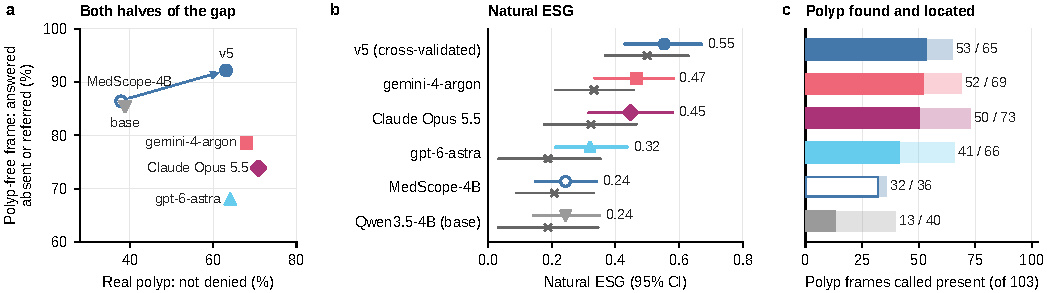
\includegraphics[width=\textwidth]{figures/fig7_natural_pairs.pdf}
\end{center}
\vspace{-0.3cm}
\caption{Natural colonoscopy pairs: nothing is edited. (a) The two halves of natural ESG on the $103$ pairs. The pre-registered \texttt{MedScope-4B} (open circle) sits on the untrained base model: it rarely claims a polyp on a polyp-free frame but denies most real polyps. The flagships deny fewer polyps and answer fewer polyp-free frames safely. Adding natural pairs to training (v5, each pair answered by a model that never saw its video) moves the model along the arrow. (b) Natural ESG with $95\%$ intervals over videos; symbols use the paired frame ($103$ pairs) and grey crosses the context frame taken $3$--$10$\,s from the polyp ($96$ pairs). (c) Polyp frames called present (pale) and called present with a box on the annotated polyp (IoU $\ge 0.3$; solid, or outlined for \texttt{MedScope-4B}); labels give both counts.}
\label{fig:natural_pairs}
\vspace{-0.2cm}
\end{figure*}

Three results follow, in the order they were obtained. (i) Without any edit, the three flagships answer $68.0$--$78.6\%$ of polyp-free frames ``absent'' or refer them ($55.2$--$66.7\%$ of frames taken seconds from a polyp), so their unsupported answers are not confined to edited images. (ii) The pre-registered \texttt{MedScope-4B} claims a polyp on few of these frames ($2$ of $103$; untrained base $15$) but finds no more real polyps than its base, so its natural ESG equals the base's ($0.243$) and, by the rule fixed in advance, its advantage does not carry over. (iii) A post hoc model trained with natural pairs reaches $0.553$ on unseen patients, above one flagship of three; this awaits independent confirmation.

\textbf{Pre-registered test: counterfactual training alone.} Table~\ref{tab:natural_pairs} and Figure~\ref{fig:natural_pairs} give the result on the $103$ colonoscopy pairs. \texttt{MedScope-4B}'s natural ESG is $0.243$ $[0.149, 0.340]$, the same as the untrained base model's ($0.243$; difference $0.000$ $[-0.103, 0.095]$) and below \texttt{gemini-4-argon} ($-0.223$ $[-0.346, -0.102]$) and \texttt{Claude Opus 5.5} ($-0.204$ $[-0.333, -0.071]$); against \texttt{gpt-6-astra} the difference is $-0.078$ $[-0.184, 0.028]$. The rule fixed in advance read ``above every flagship with the interval above zero'' as the advantage carrying over and ``above none'' as not carrying over. \texttt{MedScope-4B} is above none, so by that rule its counterfactual advantage \emph{does not carry over} to unedited images of this new source: on the registered measure it matches its base on both halves (polyps not denied $37.9\%$ against $38.8\%$; polyp-free frames answered ``absent'' or referred $86.4\%$ against $85.4\%$). On the counterfactual colonoscopy test the same model scores $0.95$. For the three flagships, which never saw our views in training, the two tests agree in order: counterfactual colonoscopy ESG $0.69$, $0.57$ and $0.40$ (Appendix Table~\ref{tab:modality_breakdown}) against natural ESG $0.466$, $0.447$ and $0.320$, each lower on the harder video frames. The counterfactual score overstates the natural one for the model trained on counterfactual views. With three models this is an observation, not a validation of the metric. Counterfactual ESG measures whether an answer is withdrawn when the evidence is removed; it does not measure whether subtle real evidence is found in images of a new source, and the two should be reported together.

The stored answers show what lies behind the equal scores. On the polyp-free frames \texttt{MedScope-4B} claims a polyp on $2$ of $103$ (base model $15$, \texttt{Claude Opus 5.5} $20$) and asks for a better image on $12$ more, which the pre-registered measure does not count as safe. On the polyp frames it calls the polyp present on $36$ of $103$ (base $40$, \texttt{Claude Opus 5.5} $73$), and on $5$ of the $34$ smallest. It answers ``absent'' without a tool call on $53$ polyp frames; on the $42$ where it zooms it finds $31$, and when it calls a polyp present its box is on the polyp in $32$ of $36$ (base: $13$ of $40$, although the base calls a tool on every polyp frame). Counterfactual training thus changed how the model errs on polyp-free frames ($2$ claims and $12$ requests for a better image, against $15$ claims for the base) but did not make it find more real polyps. One likely reason is its training set: the training polyps are large, centred still images, the lesion-free colonoscopy images are landmark frames from a different source, and every training zoom is aimed at a labelled lesion box, so the model never had to tell a subtle real polyp from the normal mucosa of the same patient.

\textbf{Natural pairs in training (v5, post hoc; cross-validated over patients).} The fold models and \texttt{v5} of Section~\ref{subsec:method_natural} were trained once each after this result. \texttt{v5} passed the guard fixed in advance on validation images (net utility $0.654$ against $0.613$ for \texttt{MedScope-4B}, limit $\ge 0.593$; lesion-free claims $9.1\%$ against $7.7\%$, limit $\le 9.7\%$). Cross-validated over patients, v5's natural ESG is $0.553$ $[0.430, 0.670]$, $+0.311$ $[0.200, 0.423]$ above \texttt{MedScope-4B}: polyps not denied rise from $37.9\%$ to $63.1\%$ and polyp-free frames answered ``absent'' or referred from $86.4\%$ to $92.2\%$. By the rule of Amendment~6 the result is \emph{mixed}: v5 is above \texttt{gpt-6-astra} ($+0.233$ $[0.096, 0.369]$, $p < 0.001$, also after Bonferroni correction for the three comparisons) and not significantly different from \texttt{gemini-4-argon} ($+0.087$ $[-0.030, 0.207]$, $p = 0.155$) or \texttt{Claude Opus 5.5} ($+0.107$ $[-0.019, 0.233]$, $p = 0.115$). Because v5 was specified after the first natural-pair result and tested on other patients of the same four centres, we treat this comparison as hypothesis-generating; it needs confirmation on an independent set with the rule fixed in advance. The models reach similar natural ESG in different ways (Figure~\ref{fig:natural_pairs}a): the flagships deny fewer polyps ($64.1$--$70.9\%$ not denied) but answer only $68.0$--$78.6\%$ of polyp-free frames ``absent'' or refer them, while v5 does so on $92.2\%$. By fold, v5's natural ESG is $0.63$, $0.49$ and $0.53$ (flagships $0.20$--$0.58$), and by centre $0.61$, $0.50$, $0.39$ and $0.75$.

Two secondary analyses, descriptive and without a reading rule, ask whether v5 finds the polyp or its context. First, a model that answers from context cannot place its box: v5 calls the polyp present with a box on it (IoU $\ge 0.3$) on $53$ of $103$ frames, against $52$, $50$ and $41$ for the three flagships, $32$ for \texttt{MedScope-4B} and $13$ for the base model. Second, against the context-matched frames ($96$ pairs) v5 answers $88.5\%$ ``absent'' or refers them where the flagships do so on $55.2$--$66.7\%$, and its natural ESG ($0.500$ $[0.367, 0.629]$) is above each flagship's with the interval above zero ($+0.167$ $[0.045, 0.280]$, $+0.177$ $[0.063, 0.292]$, $+0.312$ $[0.167, 0.446]$; $p = 0.007$, $0.004$ and $<0.001$, uncorrected). Frames taken seconds from a polyp are the ones the flagships least often answer ``absent'' or refer.

\textbf{What v5 changes elsewhere.} \texttt{v5} leaves the main test unchanged against \texttt{MedScope-4B} (ESG $0.744$ against $0.758$, $-0.014$ $[-0.062, 0.036]$; net utility $-0.025$ $[-0.082, 0.029]$; colonoscopy ESG $0.95$ for both). It is better on the external centres (net utility $+0.115$ $[0.018, 0.217]$; CCR $+0.071$ $[0.014, 0.131]$) and, on the fresh external set, in net utility ($+0.141$ $[0.044, 0.241]$) and CCR ($+0.101$ $[0.043, 0.162]$), and it finds pneumothorax on new SIIM patients as v4.2 does (ESG $0.400$, against $0.360$ for v4.2 and $0.000$ for \texttt{MedScope-4B}). It is worse in one respect. On the fresh external set it claims more erased lesions than \texttt{MedScope-4B} ($19.6\%$ against $8.3\%$, $+0.113$ $[0.052, 0.175]$) and than v4.2 ($+0.083$ $[0.031, 0.138]$); against \texttt{MedScope-4B} the increase is almost entirely on SIIM pneumothorax ($35\%$ against $0\%$; ETIS-Larib $18\%$ against $21\%$). On the external centres it claims more than v4.2 ($11.8\%$ against $6.7\%$, $p = 0.005$). Its fresh-external ESG is unchanged ($0.387$ against $0.393$), and on BraTS meningioma it is lower ($0.22$ against $0.41$). On the fresh internal chest X-ray set no difference is significant, but erased-lesion claims are higher in point estimate ($33.3\%$ against $19.4\%$). Appendix Table~\ref{tab:v5_other} gives every set.

\textbf{Chest X-ray pairs (secondary).} The chest X-ray pairs were built with two faults and do not distinguish the models as built; they are reported in \ref{app:prereg_and_funnel}.

\section{Discussion and Limitations}
\label{sec:discussion}
%%%%%%%%% DISCUSSION %%%%%%%%%

\subsection{Evidence Against an Edit-Detection Explanation}
\label{subsec:disc_shortcut}
\texttt{MedScope-4B} is trained on counterfactual views made by the same pipeline that builds the test, so the obvious alternative explanation is that it learned the pipeline rather than the lesions: that it answers ``absent'' whenever an image looks edited. Table~\ref{tab:shortcut} collects the tests already reported above that such a model would fail. An ``edited means absent'' policy denies every intact lesion after a control edit and claims the finding on every untouched image; \texttt{MedScope-4B} does neither. ESG is the rate of ``absent'' or refer answers on erasures ($90.4\%$; the other $9.6\%$ are claimed) minus the same rate on control edits, so \texttt{MedScope-4B} denies or refers on $14.6\%$ of the $219$ control-edited views whose lesion is intact. It claims the finding on $7.6\%$ of the $288$ untouched lesion-free images, where no edit exists to detect, and the gap holds where edits are hard to see (erasures a frontier model rated unedited), where both readers saw no residual finding, on two inpainting tools it never saw, and on four external datasets it never saw. On $103$ unedited polyp-free video frames of a dataset it never saw, where again no edit exists to detect, it claims a polyp on $2$ (the untrained base model on $15$).

\begin{table*}[!t]
\caption{Tests that an ``edited means absent'' shortcut would fail, collected from results reported above. Shortcut: the behaviour of a policy that says ``absent'' on every edited image and ``present'' otherwise. Frontier: the nine frontier VLMs, or the three flagships where marked $^{\ast}$. $^{\ddagger}$Stage-1 recipe on the validation cases it detects unedited ($143$); all other rows are the final \texttt{MedScope-4B}. $^{\S}$Derived from ESG and the erased-claim rate (text).}
\label{tab:shortcut}
\vspace{-0.2cm}
\begin{center}
\small
\begin{adjustbox}{max width=\linewidth}
\begin{tabular}{llccc}
\toprule
\textbf{Check} & \textbf{Views} & \textbf{Shortcut} & \textbf{\texttt{MedScope-4B}} & \textbf{Frontier} \\
\midrule
Intact lesion after a control edit elsewhere: denied or referred & $219$ (main test) & $100\%$ & $14.6\%^{\S}$ & -- \\
Intact lesion after a $2$-px ring edit at the lesion site: denied (LaMa) & $143^{\ddagger}$ & $100\%$ & $7.7\%$ (far control $4.2\%$; erasure $86.7\%$) & -- \\
Untouched lesion-free images: finding claimed & $288$ & $100\%$ & $7.6\%$ & $9.0$--$30.9\%$ \\
Erasures a frontier model rated unedited: lesion claimed & $61$ & -- & $15\%$ ($8\%$ when visibly edited) & $41$--$64\%$ \\
Reader-clean erasures / reader-confirmed healthy images: claimed & $10$ / $16$ & -- & $0/10$ / $0/16$ & $26\%$ / -- (pooled) \\
Held-out inpainting tools, ESG (TELEA / Stable Diffusion; seen LaMa $0.752$) & $125$ & -- & $0.664$ / $0.640$ & lower on every tool$^{\ast}$ \\
External centres, ESG / lesion-free claims & $169$ & -- & $0.597$ / $4\%$ & $0.277$--$0.412$ / $18$--$30\%^{\ast}$ \\
Low-visibility erasures (scored by a trained edit detector), ESG & $111$ & -- & $0.640$ & lower by $0.27$--$0.45^{\ast}$ \\
Unedited polyp-free video frames of an unseen source: polyp claimed & $103$ & $100\%$ & $2$ (untrained base: $15$) & $20$ (\texttt{Claude Opus 5.5}) \\
\bottomrule
\end{tabular}
\end{adjustbox}
\end{center}
\vspace{-0.2cm}
\end{table*}

\textbf{What remains of the shortcut.} Two results bound this conclusion. First, edits are not invisible: a supervised ResNet-18 separates control-edited from unedited images at AUC $0.83$, and the model's own encoder at $0.61$--$0.75$ (Section~\ref{subsec:exp_review}), so the shortcut is available, and the matched control edit is what removes it. It removes it fully only for tools seen in training: after an unseen TELEA edit elsewhere in the image, the training recipe denies $23.2\%$ of $125$ intact lesions (against $43.2\%$ without control edits), and $20.3\%$ after a TELEA ring at the lesion site; among the $112$ cases that both the recipe and the base model found, $12$ of the $14$ ring denials are chest X-rays. Second, \texttt{MedScope-4B} claims more erasures that a frontier model rated unedited ($15\%$) than visibly edited ones ($8\%$): those erasures may hold more residual lesion, or the model may use some edit cues; we cannot separate the two. A trained edit detector gives the same pattern ($16.2\%$ of low-visibility erasures claimed against $2.8\%$ of the others; Section~\ref{subsec:exp_review}). Three further limits concern generalization rather than edit detection (lesion-free images that share sources with training, uneven external results, and the natural-pair test); they are taken up in the Limitations.

\subsection{What Counterfactual Evaluation Can and Cannot Certify}
\label{subsec:disc_certify}
Our blinded physician reader study delivers a dual lesson for counterfactual evaluation in medical imaging. On the one hand, for focal mucosal lesions in colonoscopy, automated inpainting with LaMa reduces physician finding calls to the level of unedited healthy tissue ($1/6$ and $2/6$ vs.\ $2/6$ and $0/6$), consistent with the visual evidence having been removed. In this imaging type, nine frontier VLMs still claim $45\%$ of $83$ erased polyps while detecting $96\%$ of unedited ones---and claim $30\%$ of reader-clean erasures whose unedited counterpart they correctly detected---which suggests that frontier models often answer such questions without support in the image. An image-blind control (the question with a blank or unrelated image) was not run, so the share due to the question alone is not separated from context left in the frame.

On the other hand, across all sources (colonoscopy included), physicians call a finding present on $54.7\%$ of pooled erased reads, against $35.9\%$ ($23/64$) of their reads of unedited lesion-free images (both readers on $40.6\%$ of erased images), even though they cannot tell edited from unedited images ($\text{AUC } 0.54\text{--}0.55$); most of these residual calls fall outside colonoscopy, and in diffuse disease such as COVID-19 opacities erasure works poorly (QaTa-COV19 $\text{ESG } 0.05$). The readers did not say what they saw. Plausible sources are secondary signs outside the mask (mass effect, oedema, pleural asymmetry, acoustic shadowing) or incomplete mask coverage, but these are hypotheses; $4$ of the $13$ images both readers called positive ask the generic abnormality question and $9$ name a specific lesion. Because counterfactual training labels every erased view ``absent'', training on unverified erasures outside colonoscopy may teach a model to discount whatever residual evidence remains (though \texttt{MedScope-4B} still claims $4/13$ residual erasures vs.\ $0/10$ reader-clean ones). Furthermore, held-out editing tools introduce generator-specific failure modes: TELEA's smooth PDE patches trigger $12.9\%$ false denials on intact lesions, whereas $41/45$ false claims on Stable Diffusion erasures point at the inpainted site, which may hold residual or regenerated tissue (these erasures were not reader-checked). Consequently, unverified automated ESG cannot be treated as a pure measure of hallucination in isolation; counterfactual benchmarks must pair target erasures with symmetric controls, held-out generators, and physician reader checks.

\subsection{Implications of the Pre-Registered Negative Map, and What Improved Detection}
\label{subsec:disc_negative_map}
Across twelve training or multi-agent arms and $270$ screened decision policies with criteria declared in advance, no intervention met its criterion, and where utility rose or erased-lesion claims fell, sensitivity on intact lesions mostly moved with them (Figure~\ref{fig:threshold_vs_discrimination_map}a); we read these gains as moves of the operating point. Several arms ran on one seed with wide intervals (for example $[-0.034, 0.067]$ for tool-family training), so small gains in discrimination are not excluded. Our layer-wise linear probes are consistent with this: the read-out gap between hidden representations and behavioral answers on held-out TELEA edits is at most $+0.028$ AUROC, and the untrained \texttt{Qwen3.5-4B} base model's hidden states already separate erased from intact lesions nearly as well as the trained recipe's ($0.83\text{--}0.87$ vs.\ $0.85\text{--}0.90$). On these views a linear read-out of the hidden states finds no separation that the answers leave unused. What remains is detection: $15\%\text{--}20\%$ of real lesions are missed on unedited images, and every miss also lowers ESG. Low-rank adaptation of the encoder at two learning rates, and with layer-wise decay, did not reduce these misses (full fine-tuning was not tested), and three other frozen encoders, including the medical BiomedCLIP, hold no more of this separation than Qwen's own (Section~\ref{subsec:exp_review}); adding training coverage did reduce them (next paragraph). At the same time, naively unfreezing the vision encoder during LoRA fine-tuning either collapses the model to text-only priors ($\text{lr } 2\times 10^{-4}$) or merely shifts the threshold toward conservatism ($\text{lr } 2\times 10^{-5}$). Methodologically, a gain in utility or a drop in erased-lesion claims should be reported together with the denial rate on matched control edits, because in our experiments most such gains came with a matching change on intact lesions.

\textbf{What improved detection: coverage, not objectives.} Two post hoc models did change what the model finds on unedited images, and both changed the training data rather than the objective. Adding pneumothorax patients to every stage (v4.2) raised detection on new patients from $0/100$ to $53/100$. Adding natural same-patient pairs (v5) raised polyps not denied on unseen patients' frames from $37.9\%$ to $63.1\%$ and polyps located with a box from $32$ to $53$ of $103$. Neither changed the main test. The twelve arms that changed the objective, the adapter capacity or the decision rule moved the threshold instead. The vision encoder is frozen in every one of these models, so both gains are consistent with the language-model adapters learning to use features the encoder already provides for such images (this was not measured directly). The misses described above therefore reflect the views the model was trained on; on images of a kind it had not seen, coverage and not the encoder was the binding constraint. Both models are single-seed and post hoc, and v5 was trained on other patients of the same four centres, so this is a suggestion, not a demonstration: for a model of this size, training on counterfactual and lesion-free views goes with few claims of what is not shown, while finding subtle real evidence seems to need real same-source pairs in training. An arm with natural pairs but without counterfactual views, which would separate the two contributions, was not run.

\textbf{Limitations.} \emph{Labels.} The counterfactual label is verified only in part: two trainee physicians (one year each; one is an author) read $128$ images, their reads are consistent with the erasures in colonoscopy only, and Stable Diffusion erasures were not read. Some lesion questions ask for any abnormality ($4$ of the $13$ erased images both readers called positive, and $8$ of the expert's $17$ colonoscopy erasures), which erasing one mask does not make absent; results by question type are not reported. A pre-registered expert study on $212$ images is open, with one reader (an author) complete (interim results in Section~\ref{subsec:exp_probes_readers_failures}). The natural-pair frames are labelled by the dataset's boxes and were not re-read. \emph{Generalization.} \texttt{MedScope-4B}'s ESG is lower in chest X-ray and SLAKE CT/MRI ($0.51$ and $0.47$) than in colonoscopy ($0.95$) and on the smallest lesions ($0.545$ in the smallest area quartile); diffuse findings do not erase cleanly (QaTa-COV19 ESG $0.05$); and a finding with almost no training coverage was missed entirely (pneumothorax, $0/48$; training held $4$ pneumothorax images and validation none, so the selection rule could not detect the loss). The lesion-free images of the main test come from the same sources as the lesion-free training images, and the training splits of the standard VQA benchmarks were seen in Stage-3 replay. The advantage did not carry over to natural pairs, and the two results on unedited images that favour our approach (v4.2 and v5) come from post hoc, single-seed models: v5 was trained on other patients of the same four centres, no centre was held out, and its comparison with the flagships is mixed by its own rule. Natural pairs are shown for colonoscopy only. \emph{Strength of evidence.} The full three-stage recipe has one training seed (three for Stage~1); the registered rerun with two more seeds (R12) has not been run. Earlier versions of the agent were run on the main test before the final recipe was fixed, so the fresh cohorts are the confirmatory evidence. Registration here means commits in our own public repository. Each API model was run once at provider defaults, and the trained agent is compared with zero-shot models on views built by the pipeline it was trained on. \emph{Scope.} The tests are closed questions on public images of at most $768$\,px (the fresh-external pneumothorax films are $256$-px copies), with no task-specific detector as a baseline. In free text the advantage is not established ($36$ cases; one of the compared models served as judge). \texttt{MedScope-4B}'s stated confidence ranks its errors worse than the frontier models' (AURC $0.065$ vs.\ $0.020$--$0.033$), and its raw single-turn log-odds are not a valid cross-case score (\ref{app:detailed_tables}). The cost matrix was fixed in advance but not elicited from clinicians, and performance by age, sex or scanner is not reported.
%%%%%%%%% DISCUSSION %%%%%%%%%

\section{Conclusion}
\label{sec:conclusion}
%%%%%%%%% CONCLUSION %%%%%%%%%
We presented a counterfactual evidence framework that tests whether medical VLMs answer closed questions from the image, using matched random-site and same-site controls, held-out inpainting tools, blinded physician reads and unedited same-patient pairs. Nine frontier VLMs claim $41.1\%$ to $61.6\%$ of erased findings ($36.8\%$ to $66.2\%$ for the three flagships across six prompting regimes), including $45\%$ of erased polyps in colonoscopy, the imaging type in which physician reads were consistent with the erasures; a 4B agent trained on automatically built counterfactual views claims $9.6\%$ (ESG $0.758$). Twelve alternative objectives, capacities and system designs and $270$ decision policies did not meet their criteria, declared in advance, for better discrimination; where utility improved, sensitivity on intact lesions mostly moved with it. Linear probes find no read-out gap in the trained model and a large one in the untrained base, which counterfactual training closes. Unedited same-patient pairs then showed what the counterfactual score does not measure: the trained agent rarely claimed a polyp that was not shown but found no more real polyps than its base. Two additions to training coverage changed what the agent finds on unedited images: pneumothorax patients ($0/100$ to $53/100$ on new patients) and natural same-patient pairs (natural ESG $0.243$ to $0.553$ on unseen patients, above one flagship and not significantly different from the other two). Both are post hoc and single-seed, and confirming them on an independent set with rules fixed in advance is the next step. Automated erasures should be reader-checked by imaging type before counterfactual scores are interpreted. In our experiments, counterfactual views went with not claiming what is not shown; real same-patient pairs were needed to find what is.

\section*{Reproducibility Statement}
All pre-registration documents (including the 1 November 2026 Stage-3 selection rule, the 8 November 2026 preprint v1.0 arXiv:2611.13006 baseline \citep{gurram2026medscope}, and the pre-registered protocols for Checks C1--C4, Stage 0 ring controls, Stage 1 tool-family training, the 270-policy screening funnel, post-preprint pilots, and the review experiments R1--R9 and R12--R16 with their six amendments; the numbers R10 and R11 were not used), source code, automated quality-control scripts and physician reader study interfaces are publicly available at \url{https://github.com/bhaskargurram-ai/medscope}. The stored per-view outputs of all open-weight checkpoints and frontier API runs (evaluated 31 October 2026 under provider default settings) are in the Hugging Face release named under Data availability. Complete per-modality, per-seed, and per-arm numeric tables are provided in the Appendix.

\section*{Data availability}
All images are public; the copies used are Kvasir-SEG from \url{https://datasets.simula.no/kvasir-seg}, HyperKvasir (\texttt{SimulaMet-HOST/HyperKvasir}), SLAKE (\texttt{BoKelvin/SLAKE}), BUSI (\texttt{MedOtter/BUSI}), ChestX-Det (\texttt{MedOtter/ChestX-Det}) and TCGA-LGG (\texttt{MedOtter/TCGA-LGG-Mask}) on Hugging Face, and SIIM-ACR from Kaggle (\path{jesperdramsch/siim-acr-pneumothorax-segmentation-data}); the original sources are cited in Section~\ref{subsec:exp_setup}. Code, pre-registrations, seeds, hardware and software versions are in the repository (\url{https://github.com/bhaskargurram-ai/medscope}). The model adapters (\texttt{MedScope-4B} and the post hoc \texttt{MedScope-4B-v4.2}) and MedScope-Bench (the view manifests, without images, and every run's per-view outputs and transcripts) are released on Hugging Face (\url{https://huggingface.co/bhaskar-ai/MedScope-4B}, \url{https://huggingface.co/bhaskar-ai/MedScope-4B-v4.2} and \url{https://huggingface.co/datasets/bhaskar-ai/MedScope-Bench}); the images are rebuilt from the public sources with the repository's scripts, because the source licences differ. The natural-pair selections (REAL-Colon video and frame numbers, no images) are rebuilt by the repository's \texttt{scripts/natural\_pairs.py}. \toconfirm{add the per-view outputs of the natural-pair runs and the post hoc v5 adapters to the public release before submission} Reader-study answer keys are not released while the expert study is open.
%%%%%%%%% CONCLUSION %%%%%%%%%


\section*{CRediT authorship contribution statement}
\textbf{Bhaskar Gurram:} Conceptualization, Methodology, Software, Formal analysis, Investigation, Data curation, Visualization, Writing -- original draft, Project administration.
\textbf{Yoshitha Challagulla:} Software, Validation, Writing -- review \& editing.
\textbf{Jyothirmaye Challagulla:} Investigation (blinded trainee reader, internal medicine), Writing -- review \& editing.
\textbf{Samir C. Grover:} Investigation (blinded expert reading), Writing -- review \& editing.

\section*{Declaration of competing interest}
B.G.\ and Y.C.\ are employed as AI engineers in industry; this work was done independently, outside their employment, and received no funding, data, computing or other resources from their employer. The authors declare no other competing financial interests or personal relationships that could have appeared to influence the work reported in this paper. \toconfirm{J.C.\ and S.C.G.: any industry or advisory relationships}

\section*{Funding}
This research did not receive any specific grant from funding agencies in the public, commercial, or not-for-profit sectors.

\section*{Ethics statement}
All images come from public, de-identified datasets; no patient was contacted and no new patient data were collected. Physician readers took part voluntarily and gave consent on the reading page before starting, and their answers are stored under reader codes. Two readers are also authors (J.C., trainee round; S.C.G., expert round); both read blinded, with no access to image labels, edit types or other readers' answers. \toconfirm{whether any reader's institution requires a formal exemption}

\section*{Declaration of generative AI and AI-assisted technologies}
\toconfirm{describe honestly any use of AI tools in writing, figures or code, as the journal requires; write ``None'' only if none were used}

\section*{Acknowledgements}
We thank the second trainee reader (radiology), who prefers to remain anonymous, for taking part in the first reader round.

\bibliography{\jobname}
\bibliographystyle{plainnat}

%%%%%%%%% Appendix %%%%%%%%%
\newpage
\onecolumn
\appendix

\section{Pre-Registration Protocol, Cost Matrices, and Screening Funnel Details}
\label{app:prereg_and_funnel}

\subsection{Pre-Registration Timeline and Decision Rules}
All confirmatory experiments in this study followed pre-registered protocols committed to the public repository (\url{https://github.com/bhaskargurram-ai/medscope}) before the corresponding models or test outputs were generated:
\begin{enumerate}[leftmargin=*,nosep]
    \item \textbf{Reference Agent Selection Rule (Committed 1 November 2026):} Prior to generating v4 data or training \texttt{MedScope-4B}, Stage 3 (general-VQA replay) was pre-specified to be selected over Stage 2 (rejection-sampling fine-tuning) if and only if validation net utility satisfied $U_3 \ge U_2 - 0.02$ and validation healthy-image claims satisfied $H_3 \le H_2 + 0.02$ across the $540$ validation cases ($1,473$ views). Observed validation values were $(U_1, H_1) = (0.585, 13.6\%)$, $(U_2, H_2) = (0.610, 12.7\%)$, and $(U_3, H_3) = (0.613, 7.7\%)$. Stage 3 met both criteria and was evaluated once on every test cohort without subsequent modification.
    \item \textbf{Confirmatory Checks C1--C4:} Pre-registered to test matched vs.\ unmatched control edit geometry/tool (C1), the Stage-1 counterfactual recipe against non-counterfactual SFT followed by removal-based DPO across three seeds (C2), adding removal-based DPO on top of the Stage-1 recipe (C3), and Control-Matched Counterfactual Consistency (CMCC) against a matched-compute replay-only control across three seed pairs (C4), with main-test healthy-image claims and fresh-external ESG and net utility as pre-specified guards (C4 was registered after a favourable one-seed pilot on the same test sets).
    \item \textbf{Post-Preprint Extensions (arXiv:2611.13006 v1.0, 8 November 2026):} Following v1.0 of the preprint \citep{gurram2026medscope}, we pre-registered the Stage-0 site-matched ring control shortcut rule (flagging a site-specific shortcut if the recipe's ring denial is $\ge 0.10$, $\ge 0.05$ above its far-control denial, and $\ge 0.05$ above the base model's ring denial), the $0.05$ read-out gap threshold on linear hidden-state probes, the $\le 10\%$ residual finding criterion and $>20\%$ reader-clean frontier claim bound for the blinded physician reader study, the Stage-1 tool-family training pass rule ($\Delta\text{TELEA ESG} \ge +0.03$, $\Delta\text{TELEA control denial} \le -0.03$, $\Delta\text{LaMa ESG} \ge -0.02$, $\Delta\text{found unedited} \ge -0.03$, and $\Delta\text{lesion-free claims} \le +0.03$), and the split-validation pass rule for the $270$ decision policies.
    \item \textbf{Review Experiments and Amendments (15--21 November 2026):} The checks R1--R9 and R12--R16 of the repository document \texttt{REVIEW\_EXPERIMENTS.md} (the numbers R10 and R11 were not used) were each committed before they ran: the review checks of Section~\ref{subsec:exp_review}, the expert reader study (R5; Amendments~3 and~3a), natural pairs (R9; Amendment~4: above every flagship with the interval above zero, the advantage carries over; above none, it does not; otherwise mixed), training seeds, edit visibility, the open-ended request and reproduction from the release (R12--R15; Amendment~5), and natural pairs in training (R16; Amendment~6: the same reading applied to the cross-validated model, a validation guard, a single attempt). Outcomes: R9 not carried over; R13 met; R14 not met; R15 reproduced; R16 mixed; R12 not yet run.
\end{enumerate}

\begin{table}[!htbp]
\caption{Every analysis with a criterion declared in advance, and its outcome. C: pre-registered check. P: one-seed pilot with a go signal declared in advance. S: pre-registered secondary or interim analysis. M: multiplicity check whose family was defined after review. The post hoc models v4.2 and v5 were each tested under a rule fixed before their test results.}
\label{tab:registered_outcomes}
\begin{center}
\footnotesize
\renewcommand{\arraystretch}{0.92}
\begin{adjustbox}{max width=\linewidth}
\begin{tabular}{L{4.6cm}cL{5.2cm}L{6.0cm}}
\toprule
\textbf{Analysis} & & \textbf{Criterion declared in advance} & \textbf{Outcome} \\
\midrule
Stage-3 selection of \texttt{MedScope-4B} & C & $U_3 \ge U_2 - 0.02$ and $H_3 \le H_2 + 0.02$ on validation & Met; Stage 3 fixed as the reported model \\
Main test, $27$ primary comparisons & M & Bonferroni over ESG, erased claims and net utility against nine frontier models & All $27$ at $p \le 0.001$ \\
Fresh internal cohort & C & Run once after the model was fixed & ESG $0.472$ vs.\ $0.000$--$0.083$ \\
Fresh external cohort & C & Run once after the model was fixed & Erased claims $8.3\%$ vs.\ $31.5$--$42.3\%$; ESG above two of three flagships; net utility below \texttt{gemini-4-argon} ($-0.363$ $[-0.496, -0.233]$); pneumothorax $0/48$ \\
v4.1: Stage 3 redone with SIIM patients & C & The Stage-3 selection rule & Not met (validation lesion-free claims $10.0\%$ vs.\ $7.7\%$) \\
C1: matched vs.\ unmatched control edit & C & Registered decision rule & Inconclusive; matching not shown to matter \\
C2: recipe vs.\ removal-based DPO & C & Registered decision rule, three seeds & No difference shown on new data \\
C3: DPO on top of the recipe & C & Registered decision rule & Not met (held-out erased claims $+8.0$ points) \\
Stage 4 (conditional on C3) & C & Trained only if C3 met its rule & Not triggered \\
Selection-rule test of ESG on a new cohort & C & Registered 8 November 2026 & Not run \\
C4: CMCC vs.\ matched-compute control & C & Lower held-out erased claims; two guards & Not met ($+0.011$ $[-0.009, 0.030]$); main-test guard failed \\
Rank-64 adapters; vision LoRA at two learning rates; GRPO & P & Go signals & Not met (GRPO narrowly) \\
Multi-agent readers v10 and v11 & P & Go/no-go rules & No go, twice \\
Tool-family training (two arms) & P & TELEA ESG $+0.03$ and control denial $-0.03$, with three guards & Not met \\
$270$ decision policies & C & Pass on half A and confirm on half B & None passed \\
Same-site ring control & C & Site flag: ring denial $\ge 0.10$, and $\ge 0.05$ over the far control and over the base model & Flag met on TELEA only; site-specific interaction $+0.018$ $[-0.080, 0.116]$ (post hoc) \\
Read-out gap (hidden-state probes) & C & Gap of at least $0.05$ AUROC & Not found ($\le 0.028$) \\
Trainee readers: residual finding & C & Upper $95\%$ bound of erased reads with a finding at most $10\%$ & Not met ($54.7\%$ pooled; lesion-free reads $35.9\%$); consistent in colonoscopy \\
Reader-clean erasures: frontier claims & C & Lower bound above $20\%$ & Not met ($26\%$ $[10, 42]$, $n = 10$) \\
R1: CORAL-style swap term & C & TELEA ESG $+0.03$ & Not met \\
R2: vision LoRA with layer-wise decay & C & Unedited lesions found $+0.03$ & Not met \\
R3: other frozen encoders & C & Better by $0.05$ with the interval above zero & None \\
R4: abstention ceiling, measured & C & No read-out gap if the bound is within $0.05$ of the denial gap & No gap: answers use the separation a linear read-out finds \\
R6: Med-CAP-style prior subtraction & C & TELEA AUROC $+0.03$ with the interval above zero & Not met \\
R7: leakage worst case & C & Advantage remains without the most similar cases & Met (smallest advantage $+0.306$ $[0.200, 0.405]$) \\
R8: v4.2 (post hoc model) & C & Validation rule fixed before its test results & Met \\
R5: expert readers, interim (one reader) & S & Upper $95\%$ bound of colonoscopy erasures called present at most $10\%$ & Cannot be judged ($4/17$); study open \\
R9: natural pairs, \texttt{MedScope-4B} & C & Above every flagship with the interval above zero & Not carried over (above none) \\
R13: edit visibility & C & Above each flagship on low-visibility erasures & Met \\
R14: open-ended request & C & Above each flagship with the interval above zero & Not met ($36$ cases) \\
R15: reproduction from the public release & C & ESG within $0.02$; at least $97\%$ of decisions identical & Met ($0.763$; $98.8\%$) \\
R16: v5 with natural pairs (post hoc model) & C & Validation guard; the R9 reading on the cross-validated model & Guard passed; mixed (above one flagship of three) \\
R12: training seeds of the full recipe & C & Every seed above each flagship & Not yet run \\
\bottomrule
\end{tabular}
\end{adjustbox}
\end{center}
\end{table}

\subsection{Alternative Clinical Cost Matrices and Abstention Ceiling Details}
To ensure that \texttt{MedScope-4B}'s Net Utility advantage over frontier and open-weight baselines is not an artifact of the specific reward weights in Table~\ref{tab:cost_matrix}, we re-scored all models under five cost matrices: the published one with the wrong-answer penalty at $-2$, $-1$ and $-0.5$, and two referral variants (referral on lesion-free images paid $0$; referral paid $-0.3$ on every view). \texttt{MedScope-4B} ranked first among all compared models under all five. The trivial always-refer policy scores $+0.110$ under the published matrix, $-0.118$ when referral on lesion-free images pays $0$, and $-0.300$ when referral pays $-0.3$ everywhere.

Under Proposition~1 (Section~\ref{subsec:method_metrics}), any post-hoc decision rule $\pi(S)$ mapping signal vector $S$ to discrete actions satisfies $\text{ESG}(\pi) \le \text{TV}(P(S \mid E), P(S \mid C_{\text{far}}))$. In our 270-policy screening funnel on the validation set (split into equal halves A and B), a policy passed only if it achieved $\Delta\text{Net Utility} \ge +0.03$, $\Delta\text{ESG} \ge +0.02$, $\Delta\text{CCR} \ge -0.03$, and $\Delta\text{lesion-free claims} \le +0.03$ on Half A and confirmed on Half B:
\begin{itemize}[leftmargin=*,nosep]
    \item \textbf{Stage A (128 policies on stored outputs):} Combined the stored outputs of the Stage-1 recipe, the question-blind reader, the dedicated lesion segmenter, and the erase-and-re-ask verifier using threshold rules, regularized logistic regression, gradient-boosted decision trees, and confidence referral bands. While $19/128$ policies passed on Half A, $0/19$ confirmed on Half B (best Half-B utility rose from $0.539$ to $0.706$ by cutting erased claims from $11.2\%$ to $3.9\%$ at the cost of CCR dropping from $0.773$ to $0.727$, with $\Delta\text{ESG} \le +0.026$).
    \item \textbf{Stage B (142 policies on new test-time evidence):} Incorporated three test-time altered image copies (horizontal mirror, center crop, contrast adjustment), a high-resolution close-up of the claimed region paired with an equal-area control close-up, a cautious prompt re-ask, first-token answer probabilities, a secondary VLM (\texttt{Qwen2.5-VL-7B}), and the lesion segmenter score. Exactly $0/142$ policies passed even on Half A: on unseen TELEA views, combiners raised net utility from $0.444$ up to $0.686$ via increased referral/abstention, while ESG stayed between $0.55$ and $0.61$ for most combiners (largest $0.642$, at a cut-off that failed elsewhere) compared to $0.600$ for the unmodified recipe.
\end{itemize}



\begin{table}[!htbp]
\caption{Checks added after the external review (pre-registered). Top: training arms on the validation dev set ($179$ lesion cases, $80$ lesion-free images), difference from the comparator paired by case with $95\%$ bootstrap intervals. Bottom: erasure vs.\ control edit, linear-probe AUC on main-test views by frozen encoder (whole image / lesion crop).}
\label{tab:review_checks}
\begin{center}
\small
\begin{adjustbox}{max width=\linewidth}
\begin{tabular}{lcc}
\toprule
\textbf{Quantity} & \textbf{Hard-negative swap vs.\ replay control} & \textbf{Vision LoRA, layer decay vs.\ recipe} \\
\midrule
Unedited lesions found & $+0.017$ $[-0.011, 0.045]$ & $+0.017$ $[-0.034, 0.067]$ \\
Lesion-free images claimed & $+0.013$ $[0.000, 0.037]$ & $-0.075$ $[-0.150, 0.000]$ \\
ESG, LaMa & $+0.011$ $[-0.022, 0.050]$ & $+0.061$ $[-0.011, 0.134]$ \\
ESG, TELEA (held out) & $-0.028$ $[-0.073, 0.017]$ & $+0.034$ $[-0.028, 0.101]$ \\
Control edit denied (found), TELEA & $+0.029$ $[0.000, 0.064]$ & $0.000$ $[-0.053, 0.053]$ \\
Ring edit denied (found), TELEA & $-0.014$ $[-0.036, 0.000]$ & $+0.075$ $[0.030, 0.128]$ \\
Pre-registered rule & not met & not met \\
\bottomrule
\end{tabular}
\end{adjustbox}

\vspace{0.2cm}
\begin{adjustbox}{max width=\linewidth}
\begin{tabular}{lccc}
\toprule
\textbf{Encoder (frozen)} & \textbf{LaMa} & \textbf{TELEA (held out)} & \textbf{Stable Diffusion (held out)} \\
\midrule
Qwen3.5-4B vision encoder & $0.859$ / $0.898$ & $0.856$ / $0.873$ & $0.798$ / $0.841$ \\
BiomedCLIP & $0.812$ / $0.884$ & $0.799$ / $0.859$ & $0.781$ / $0.831$ \\
DINOv2-base & $0.730$ / $0.823$ & $0.688$ / $0.742$ & $0.666$ / $0.747$ \\
RAD-DINO & $0.710$ / $0.764$ & $0.671$ / $0.645$ & $0.666$ / $0.669$ \\
\bottomrule
\end{tabular}
\end{adjustbox}
\end{center}
\end{table}

\begin{table}[!htbp]
\caption{The post hoc model \texttt{v5} (natural pairs in training, all $60$ videos) on the earlier tests, paired with \texttt{MedScope-4B} (v4) and with v4.2 over the same cases; differences are \texttt{v5} minus the other model with $95\%$ bootstrap intervals, in bold when the interval excludes zero. Erased and lesion-free claims: lower is better. Standard VQA accuracy (all questions; \texttt{v5} / v4.2 / v4): VQA-RAD $0.517$ / $0.539$ / $0.514$; SLAKE $0.747$ / $0.750$ / $0.730$; PathVQA $0.503$ / $0.487$ / $0.477$.}
\label{tab:v5_other}
\begin{center}
\small
\begin{adjustbox}{max width=\linewidth}
\begin{tabular}{llccccc}
\toprule
\textbf{Test (cases)} & \textbf{Metric} & \textbf{v5} & \textbf{v4} & \textbf{v5 $-$ v4} & \textbf{v4.2} & \textbf{v5 $-$ v4.2} \\
\midrule
Main test ($507$) & Net utility & $0.707$ & $0.732$ & $-0.025$ $[-0.082, 0.029]$ & $0.714$ & $-0.007$ $[-0.054, 0.038]$ \\
 & ESG & $0.744$ & $0.758$ & $-0.014$ $[-0.062, 0.036]$ & $0.740$ & $+0.005$ $[-0.044, 0.051]$ \\
 & CCR & $0.854$ & $0.849$ & $+0.005$ $[-0.026, 0.036]$ & $0.856$ & $-0.002$ $[-0.027, 0.022]$ \\
 & Erased claims & $11.0\%$ & $9.6\%$ & $+0.014$ $[-0.027, 0.055]$ & $11.0\%$ & $0.000$ $[-0.036, 0.035]$ \\
 & Lesion-free claims & $8.7\%$ & $7.6\%$ & $+0.010$ $[-0.021, 0.042]$ & $9.0\%$ & $-0.003$ $[-0.034, 0.026]$ \\
\midrule
External centres ($169$) & Net utility & $0.645$ & $0.530$ & $\mathbf{+0.115}$ $\mathbf{[0.018, 0.217]}$ & $0.696$ & $-0.050$ $[-0.131, 0.032]$ \\
 & ESG & $0.681$ & $0.597$ & $+0.084$ $[-0.000, 0.172]$ & $0.739$ & $-0.059$ $[-0.132, 0.017]$ \\
 & CCR & $0.798$ & $0.727$ & $\mathbf{+0.071}$ $\mathbf{[0.014, 0.131]}$ & $0.815$ & $-0.017$ $[-0.068, 0.036]$ \\
 & Erased claims & $11.8\%$ & $11.8\%$ & $0.000$ $[-0.050, 0.052]$ & $6.7\%$ & $\mathbf{+0.050}$ $\mathbf{[0.017, 0.095]}$ \\
 & Lesion-free claims & $2.0\%$ & $4.0\%$ & $-0.020$ $[-0.093, 0.042]$ & $6.0\%$ & $-0.040$ $[-0.104, 0.000]$ \\
\midrule
Fresh internal ($76$) & Net utility & $0.484$ & $0.402$ & $+0.082$ $[-0.176, 0.349]$ & $0.500$ & $-0.016$ $[-0.192, 0.143]$ \\
 & ESG & $0.500$ & $0.472$ & $+0.028$ $[-0.189, 0.270]$ & $0.528$ & $-0.028$ $[-0.154, 0.103]$ \\
 & CCR & $0.819$ & $0.681$ & $+0.139$ $[-0.029, 0.324]$ & $0.778$ & $+0.042$ $[-0.088, 0.167]$ \\
 & Erased claims & $33.3\%$ & $19.4\%$ & $+0.139$ $[-0.026, 0.296]$ & $25.0\%$ & $+0.083$ $[0.000, 0.184]$ \\
 & Lesion-free claims & $20.0\%$ & $12.5\%$ & $+0.075$ $[-0.095, 0.244]$ & $17.5\%$ & $+0.025$ $[-0.105, 0.158]$ \\
\midrule
Fresh external ($316$) & Net utility & $0.088$ & $-0.053$ & $\mathbf{+0.141}$ $\mathbf{[0.044, 0.241]}$ & $0.048$ & $+0.040$ $[-0.048, 0.128]$ \\
 & ESG & $0.387$ & $0.393$ & $-0.006$ $[-0.074, 0.058]$ & $0.417$ & $-0.030$ $[-0.088, 0.032]$ \\
 & CCR & $0.577$ & $0.476$ & $\mathbf{+0.101}$ $\mathbf{[0.043, 0.162]}$ & $0.536$ & $+0.042$ $[-0.006, 0.092]$ \\
 & Erased claims & $19.6\%$ & $8.3\%$ & $\mathbf{+0.113}$ $\mathbf{[0.052, 0.175]}$ & $11.3\%$ & $\mathbf{+0.083}$ $\mathbf{[0.031, 0.138]}$ \\
 & Lesion-free claims & $4.1\%$ & $4.7\%$ & $-0.007$ $[-0.042, 0.028]$ & $6.8\%$ & $-0.027$ $[-0.066, 0.008]$ \\
\midrule
New SIIM patients ($200$) & Net utility & $-0.028$ & $-1.100$ & $\mathbf{+1.072}$ $\mathbf{[0.873, 1.263]}$ & $-0.096$ & $+0.068$ $[-0.116, 0.253]$ \\
 & ESG & $0.400$ & $0.000$ & $\mathbf{+0.400}$ $\mathbf{[0.299, 0.500]}$ & $0.360$ & $+0.040$ $[-0.060, 0.140]$ \\
 & CCR & $0.585$ & $0.000$ & $\mathbf{+0.585}$ $\mathbf{[0.490, 0.670]}$ & $0.540$ & $+0.045$ $[-0.043, 0.131]$ \\
 & Erased claims & $20.0\%$ & $0.0\%$ & $\mathbf{+0.200}$ $\mathbf{[0.125, 0.280]}$ & $19.0\%$ & $+0.010$ $[-0.063, 0.083]$ \\
 & Lesion-free claims & $7.0\%$ & $0.0\%$ & $\mathbf{+0.070}$ $\mathbf{[0.021, 0.125]}$ & $5.0\%$ & $+0.020$ $[0.000, 0.052]$ \\
\bottomrule
\end{tabular}
\end{adjustbox}
\end{center}
\end{table}

\paragraph{Chest X-ray natural pairs (secondary; not informative as built).} The chest X-ray pairs of Section~\ref{subsec:method_natural} were built with two deviations, found during the run after one model's chest X-ray result had been seen: the exclusion of ChestX-Det patients matched no patient, and a near-copy check that compared coarse image hashes without confirming them dropped $156$ of $200$ pairs. We report the $44$ remaining pairs as run, for completeness: natural ESG is $0.068$ $[-0.068, 0.205]$ for \texttt{MedScope-4B}, $0.068$ for v4.2 and the base model, and $0.045$ to $0.159$ for the flagships, and every difference from \texttt{MedScope-4B} includes zero (by finding, \texttt{MedScope-4B}: effusion $0.00$, mass $0.50$, nodule $-0.14$, pneumothorax $-0.06$). With $44$ pairs and labels mined from reports, this set does not distinguish the models and we draw no conclusion from it; a rebuild with the check corrected is specified and has not been run.

\paragraph{Where \texttt{MedScope-4B}'s errors concentrate.} Its errors concentrate in six places: small real polyps in video frames of a new source ($5$ of the $34$ smallest found, against $19$ for \texttt{Claude Opus 5.5}); the smallest lesions (ESG $0.545$ and $18.2\%$ erased claims in the smallest area quartile); chest X-ray and SLAKE CT/MRI (ESG $0.51$ and $0.47$, against $0.95$ in colonoscopy); diffuse findings, which do not erase cleanly (QaTa-COV19 ESG $0.05$); rare findings absent from training and validation (pneumothorax, $0/48$); and denial of intact lesions after an unfamiliar edit near them, concentrated in chest X-rays ($12$ of $17$ chest X-ray cases denied after a TELEA ring). By finding, it misses fibrosis ($3/4$) and tumour ($5/23$) on the main test and tumour ($11/20$) and the generic abnormality question ($12/32$) on the fresh external set, besides pneumothorax. Its stated confidence also ranks its errors worse than the frontier models' (AURC $0.065$ vs.\ $0.020$--$0.033$).

\section{Reporting Checklist (CLAIM)}
\label{app:claim}
Table~\ref{tab:claim} maps the manuscript to the Checklist for Artificial Intelligence in Medical Imaging \citep{mongan2020claim}, 2024 update \citep{tejani2024claim}, grouped by the checklist's sections.

\begin{table}[!htbp]
\caption{Where each part of the CLAIM 2024 checklist is addressed.}
\label{tab:claim}
\begin{center}
\small
\begin{adjustbox}{max width=\linewidth}
\begin{tabular}{L{3.6cm}L{9.6cm}}
\toprule
\textbf{Checklist section} & \textbf{Where and how it is addressed} \\
\midrule
Title, abstract & Title; abstract (design, data, main results with intervals). \\
Introduction: background, objectives, hypotheses & Section~\ref{sec:intro}: clinical context, the three confounds, the hypothesis (a)--(f). \\
Study design and intended use & Retrospective study of public, de-identified datasets; an evaluation framework and a research reference agent, not a clinical device (Sections~\ref{sec:method}, \ref{subsec:exp_setup}). \\
Data sources, selection, preprocessing & Sources and counts (Section~\ref{subsec:exp_setup}, Table~\ref{tab:datasets_overview}); lesions under 20\,px or over $20\%$ of the image excluded; yes/no presence questions; automatic quality control (Section~\ref{subsec:method_views}); images as PNG, long side at most 768\,px. \\
De-identification & Public releases, de-identified by their providers; no new patient data were collected; the reader study used the same images. \\
Missing data & Cases failing quality control or an edit are dropped with both edited views (counts in Section~\ref{subsec:exp_setup}); held-out-tool cases are dropped if either edit fails its check. \\
Imaging parameters & As released by each source; not available per image (Section~\ref{sec:discussion}, limitation 5). \\
Reference standard & Expert lesion masks of the source datasets; counterfactual labels derived automatically; checked by two blinded trainee physicians with agreement statistics (Section~\ref{subsec:exp_probes_readers_failures}, \ref{app:detailed_tables}). \\
Data partitions and independence & Patient or near-copy-group splits, cross-set audit, patient-level bootstrap (Section~\ref{subsec:exp_setup}, ``Data leakage and patient-level splits''). \\
Test-set size & Fixed by the available cases and pre-registered, not by a power analysis. \\
Model, software, initialization & \texttt{Qwen3.5-4B} with rank-16 LoRA, frozen vision encoder; software versions; initialized from the public base model (Section~\ref{subsec:method_agent}). \\
Training and model selection & Hyperparameters and stages (Section~\ref{subsec:method_agent}); pre-registered selection rule; no ensembling (the multi-agent systems are separate, compared arms). \\
Metrics and statistics & ESG, claims, CCR, grounding, net utility, AUROC (Section~\ref{subsec:method_metrics}); case-clustered bootstrap, paired tests, Bonferroni over 27 primary comparisons (Section~\ref{subsec:exp_setup}). \\
Robustness and interpretability & Prompts, wordings, cost matrices, editing tools, lesion size (Section~\ref{subsec:exp_main}); evidence boxes; layer-wise probes (Section~\ref{subsec:exp_probes_readers_failures}). \\
Internal and external testing & Main test; external centres, fresh internal and fresh external cohorts (Section~\ref{subsec:exp_probes_readers_failures}, Appendix Table~\ref{tab:generalization_and_pneumo}); unedited same-patient pairs of an unseen source (Section~\ref{subsec:exp_natural}). \\
Registration & Pre-registration documents committed to the public repository before each check; no clinical trial. \\
Data flow and demographics & Counts per source and cohort (Table~\ref{tab:datasets_overview}); demographics not compiled (limitation 5). \\
Performance and errors & Tables with intervals; errors by imaging type, editing tool and lesion size; the pneumothorax audit; reader-verified re-scoring. \\
Discussion & Limitations and implications (Section~\ref{sec:discussion}). \\
Protocols, code, data & Reproducibility Statement: pre-registrations, code, per-view outputs. \\
Funding & No external funding. \\
\bottomrule
\end{tabular}
\end{adjustbox}
\end{center}
\end{table}

\section{Complete Per-Arm Numeric Tables, Log-Odds Analysis, and Reader Study Protocol}
\label{app:detailed_tables}

\subsection{Stage-1 Ablations, Held-Out Tools, Negative Map, Ring Controls, Reader Study, and External Generalization}
Tables~\ref{tab:ablations_and_factorial} through \ref{tab:generalization_and_pneumo} provide the complete numeric results for the Stage-1 training ablations, the $2\times 2$ factorial decomposition, the held-out inpainting tools evaluation, the pre-registered negative map summary, the Stage-0 same-site ring controls and hidden-state linear probes, the blinded physician reader study, and the external generalization and SIIM pneumothorax breakdown discussed in Section~\ref{sec:experiments}.

\begin{table}[!htbp]
\caption{Stage-1 counterfactual training ablations ($507$ main-test cases; 3-seed arms reported as $\text{mean} \pm \text{sd}$) and the $2\times 2$ factorial ablation of training-only components (Stage 1, seed 0) evaluating false denial of intact lesions when unseen TELEA edits occur elsewhere on the image ($125$ cases).}
\label{tab:ablations_and_factorial}
\begin{center}
\small
\resizebox{\linewidth}{!}{%
\begin{tabular}{lccccc}
\toprule
\textbf{A. Stage-1 Training Arm (Main Test, $n=507$)} & \textbf{CCR} $\uparrow$ & \textbf{ESG} $\uparrow$ & \textbf{Erased \%} $\downarrow$ & \textbf{Healthy \%} $\downarrow$ & \textbf{Net Utility} $\uparrow$ \\
\midrule
Qwen3.5-4B, with counterfactual views (3 seeds) & $0.871 \pm 0.022$ & $0.741 \pm 0.019$ & $13.2 \pm 3.2$ & $13.9 \pm 4.0$ & $0.684 \pm 0.021$ \\
Qwen3.5-4B, without CF views (3 seeds) & $0.955 \pm 0.008$ & $0.279 \pm 0.107$ & $67.6 \pm 11.9$ & $35.9 \pm 3.9$ & $0.341 \pm 0.090$ \\
Without CF, ``absent'' share matched (seed 0) & $0.945$ & $0.215$ & $73.5$ & $31.6$ & $0.321$ \\
Erasures only (seed 0) & $0.788$ & $0.708$ & $6.8$ & $5.9$ & $0.667$ \\
Control edits only, matched (seed 0) & $0.897$ & $0.744$ & $15.1$ & $11.8$ & $0.727$ \\
Control edits only, unmatched (seed 0) & $0.904$ & $0.753$ & $15.1$ & $12.5$ & $0.739$ \\
Without CF, then removal-based DPO (3 seeds) & $0.903 \pm 0.014$ & $0.661 \pm 0.037$ & $24.2 \pm 5.3$ & $19.4 \pm 4.3$ & $0.637 \pm 0.033$ \\
\midrule
MedGemma 1.5 4B, with CF views & $0.806$ & $0.721$ & $7.8$ & $5.9$ & $0.698$ \\
MedGemma 1.5 4B, without CF views & $0.947$ & $0.374$ & $57.5$ & $31.6$ & $0.409$ \\
MedGemma 1.5 4B, untrained & $0.674$ & $0.283$ & $54.3$ & $24.0$ & $-0.255$ \\
\bottomrule
\end{tabular}%
}

\vspace{0.2cm}
\resizebox{\linewidth}{!}{%
\begin{tabular}{cc|cccc|c}
\toprule
\multicolumn{2}{c|}{\textbf{B. $2\times 2$ Factorial (Seed 0)}} & \multicolumn{4}{c|}{\textbf{Main Test ($n=507$)}} & \textbf{Unseen TELEA ($n=125$)} \\
\textbf{Control Edits} & \textbf{Insertions} & \textbf{CCR} $\uparrow$ & \textbf{ESG} $\uparrow$ & \textbf{Erased \%} $\downarrow$ & \textbf{Healthy \%} $\downarrow$ & \textbf{Denies Intact Lesion \%} $\downarrow$ \\
\midrule
no & no (erasures only) & $0.788$ & $0.708$ & $6.8$ & $5.9$ & $43.2$ \\
no & yes & $0.806$ & $0.735$ & $7.3$ & $11.1$ & $43.2$ \\
yes & no & $0.897$ & $0.744$ & $15.1$ & $11.8$ & $\mathbf{16.0}$ \\
yes & yes (full recipe) & $0.847$ & $0.735$ & $11.9$ & $9.4$ & $\mathbf{23.2}$ \\
\bottomrule
\end{tabular}%
}
\end{center}
\end{table}

\begin{table}[!htbp]
\caption{Generalization across seen training inpainting tools (LaMa, Tissue Transplant) and unseen held-out tools (TELEA, Stable Diffusion) on $125$ main-test cases (top; reported as $\text{ESG} \;/\; \text{Erased-lesion claims \%}$), and diagnostic breakdown of where the Stage-1 recipe's ESG is lost across $219$ pooled main-test cases (bottom).}
\label{tab:heldout_tools}
\begin{center}
\small
\begin{adjustbox}{max width=\linewidth}
\begin{tabular}{lcccc}
\toprule
\textbf{A. Model ($n=125$ cases)} & \textbf{LaMa (Seen)} & \textbf{Transplant (Seen)} & \textbf{TELEA (Unseen)} & \textbf{Diffusion (Unseen)} \\
\midrule
\textbf{MedScope-4B} & \textbf{0.752} / \textbf{7.2} & \textbf{0.720} / \textbf{8.0} & \textbf{0.664} / \textbf{7.2} & \textbf{0.640} / \textbf{17.6} \\
gemini-4-argon & 0.536 / 32.8 & 0.488 / 32.8 & 0.560 / 8.8 & 0.392 / 40.0 \\
Claude Opus 5.5 & 0.376 / 45.6 & 0.264 / 56.8 & 0.296 / 41.6 & 0.352 / 46.4 \\
gpt-6-astra & 0.312 / 55.2 & 0.240 / 64.0 & 0.256 / 60.8 & 0.256 / 61.6 \\
\midrule
Stage 1, full recipe & 0.720 / 12.0 & 0.744 / 8.0 & 0.696 / 7.2 & 0.568 / 24.8 \\
Stage 1, control edits only & 0.712 / 17.6 & 0.736 / 9.6 & 0.768 / 7.2 & 0.704 / 16.0 \\
Stage 1, insertions only & 0.696 / 6.4 & 0.664 / 4.8 & 0.512 / 5.6 & 0.600 / 11.2 \\
Stage 1, erasures only & 0.688 / 7.2 & 0.656 / 4.8 & 0.544 / 2.4 & 0.712 / 4.8 \\
Stage 1, without CF views & 0.272 / 69.6 & 0.200 / 76.8 & 0.144 / 83.2 & 0.232 / 73.6 \\
\bottomrule
\end{tabular}
\end{adjustbox}

\vspace{0.2cm}
\resizebox{\linewidth}{!}{%
\begin{tabular}{lccccc}
\toprule
\textbf{B. Tool ($n=219$, Stage-1 Recipe)} & \textbf{Denies $E$} & \textbf{Denies $C_{\text{far}}$} & \textbf{ESG} & \textbf{Denies $C_{\text{far}}$ (Found on $O$)} & \textbf{Erased Claims at Site} \\
\midrule
LaMa (training) & 0.881 & 0.146 & 0.735 & 0.027 (5/186) & 9/22 \\
TELEA (held out) & 0.918 & 0.219 & 0.699 & 0.129 (24/186; 13 breast US) & 11/13 \\
Stable Diffusion (held out) & 0.743 & 0.152 & 0.592 & 0.043 (7/162) & 41/45 \\
\bottomrule
\end{tabular}%
}
\end{center}
\end{table}

\begin{table}[!htbp]
\caption{Summary of pre-registered checks (C1--C4), post-preprint training and multi-agent pilots, Stage-1 tool-family training, and the $270$-policy validation screening funnel. Every intervention shifts the answer/abstention threshold along the sensitivity--specificity trade-off without passing pre-registered criteria for improved held-out discrimination. $^{\ast}$Held-out comparisons against the replay-only control; CCR guards against the Stage-1 recipe.}
\label{tab:negative_map_summary}
\begin{center}
\small
\resizebox{\linewidth}{!}{%
\begin{tabular}{llp{6.0cm}l}
\toprule
\textbf{Arm / Check} & \textbf{Control Baseline} & \textbf{Key Empirical Result (Held-Out Tools / External)} & \textbf{Verdict} \\
\midrule
\textbf{C1}: Matched vs.\ unmatched ctrl & Unmatched ctrl & Main ESG $0.744$ vs.\ $0.753$; Held-out ESG $0.749$ vs.\ $0.761$ (within seed noise; unmatched has bias on SIIM) & Inconclusive \\
\textbf{C2}: Recipe vs.\ No-CF + DPO & No-CF + DPO (3s) & Fresh-ext ESG $0.381 \pm 0.018$ vs.\ $0.355 \pm 0.015$ (DPO trades lower sensitivity $0.485$ vs.\ $0.587$ for fewer erased claims) & No difference \\
\textbf{C3}: Recipe + removal DPO & Stage-1 Recipe & Held-out ESG drops $0.649 \to 0.595$; erased claims rise $16.3\% \to 24.4\%$ ($+0.080$ $[0.046, 0.118]$) & \textbf{Fails} \\
\textbf{C4}: CMCC consistency loss & Replay ctrl (3s) & Pooled held-out ESG $+0.020$ ($p=0.143$); shifts all endpoints to ``present'' (fresh-ext erased $+0.073$, $p<0.001$) & \textbf{Fails} \\
\midrule
Adapter capacity (LoRA $r=64$) & Stage-1 Recipe & Main ESG $0.731$ vs.\ $0.735$; calls $25/48$ SIIM pneumothorax but $21/48$ erased \& $12/48$ healthy (SIIM ESG $0.042$) & No go (bias) \\
Vision Encoder LoRA ($\text{lr } 2\text{e-}4$) & Stage-1 Recipe & $\text{ESG} = 0.000$ on every set; collapses to answering from question text alone & \textbf{Collapse} \\
Vision Encoder LoRA ($\text{lr } 2\text{e-}5$) & Stage-1 Recipe & Main ESG $0.776$, but fresh-ext CCR drops $0.560 \to 0.488$ ($-0.071$, $p=0.03$); erased $6.8\%$ (more conservative) & No go \\
GRPO on cost matrix (150 steps) & Replay ctrl & Held-out utility $+0.056$, erased $+0.022$; go signal on erased claims missed; fresh-ext utility $+0.124$, ESG $+0.083$, healthy claims $+0.054$ & Narrowly missed \\
Multi-Agent Reader v10 & Replay ctrl$^{\ast}$ & Held-out utility $+0.090$ $[+0.004, +0.180]$; external CCR drops $0.769 \to 0.513$, fresh-ext CCR $0.560 \to 0.378$ & No go \\
Multi-Agent Reader v11 & Replay ctrl$^{\ast}$ & Main utility $0.809$ (uses LaMa verifier), but held-out ESG $-0.002$, erased claims $+0.061$ $[+0.027, +0.096]$ & No go \\
Tool-family replay (Stage 1) & Replay ctrl & Val TELEA ESG $0.665$ vs.\ $0.648$ ($+0.017$ $[-0.034, 0.067]$); LaMa ESG $-0.022$; TELEA ctrl denial $-0.021$ & \textbf{Fails} (rules 1--3) \\
Tool-family + CMCC (Stage 1) & Replay ctrl & Val TELEA ESG $0.659$ vs.\ $0.648$ ($+0.011$); lesion-free claims $+0.075$ $[0.013, 0.150]$; ring denial $+0.061$ & \textbf{Fails} (rules 1,2,5) \\
\midrule
\textbf{Stage A}: 128 stored-output rules & Validation split A/B & $19/128$ pass Half A, $\mathbf{0/19}$ confirm on Half B (utility $0.539 \to 0.706$ via referral, $\Delta\text{ESG} \le +0.026$) & \textbf{0 confirmed} \\
\textbf{Stage B}: 142 test-time combiners & Validation split A/B & $\mathbf{0/142}$ pass Half A (TELEA utility $0.444 \to 0.686$ by abstaining; ESG mostly $0.55\text{--}0.61$, at most $0.642$, vs.\ $0.600$ recipe) & \textbf{0 confirmed} \\
\bottomrule
\end{tabular}%
}
\end{center}
\end{table}

\begin{table}[!htbp]
\caption{Stage-0 site-matched control evaluation (top; denial rates among validation cases found on the unedited image: $n=143$ Recipe, $n=127$ Base) and $5$-fold cross-validated AUROC of layer-wise logistic regression linear probes on hidden states (bottom; trained on LaMa views across $8$ layers).}
\label{tab:ring_and_probes}
\begin{center}
\small
\resizebox{\linewidth}{!}{%
\begin{tabular}{llccccccccccc}
\toprule
\textbf{A. Model} & \textbf{Tool} & \textbf{Found $O$} & \textbf{Far} & \textbf{Ring} & \textbf{Rest.} & \textbf{Part.} & \textbf{Erased} & \textbf{Ring$-$Far} & $\textbf{ESG}_{\text{far}}$ & $\textbf{ESG}_{\text{site}}$ & $\textbf{AUC}_{\text{far}}$ & $\textbf{AUC}_{\text{site}}$ \\
\midrule
Recipe & LaMa & 0.799 & 0.042 & 0.077 & 0.070 & 0.196 & 0.867 & $+0.035$ & 0.665 & 0.648 & 0.853 & 0.845 \\
Recipe & TELEA & 0.799 & 0.126 & 0.203 & 0.140 & -- & 0.923 & $+0.077$ & 0.654 & 0.642 & 0.847 & 0.824 \\
Base & LaMa & 0.709 & 0.023 & 0.047 & -- & -- & -- & $+0.023$ & -- & -- & -- & -- \\
Base & TELEA & 0.709 & 0.070 & 0.116 & -- & -- & -- & $+0.047$ & -- & -- & -- & -- \\
\bottomrule
\end{tabular}%
}

\vspace{0.2cm}
\resizebox{\linewidth}{!}{%
\begin{tabular}{llcccc}
\toprule
\textbf{B. Linear Probe Task} & \textbf{Test Tool} & \textbf{Recipe (Last Token)} & \textbf{Recipe (Image Tokens)} & \textbf{Base (Last Token)} & \textbf{Base (Image Tokens)} \\
\midrule
Erased ($E$) vs.\ Ring ($C_{\text{ring}}$) & LaMa & 0.898 & 0.901 & 0.829 & 0.870 \\
Erased ($E$) vs.\ Ring ($C_{\text{ring}}$) & TELEA & 0.816 & 0.852 & 0.808 & 0.831 \\
Erased ($E$) vs.\ Far ($C_{\text{far}}$) & LaMa & 0.898 & 0.887 & 0.827 & 0.853 \\
Erased ($E$) vs.\ Far ($C_{\text{far}}$) & TELEA & 0.812 & 0.851 & 0.771 & 0.804 \\
Ring ($C_{\text{ring}}$) vs.\ Original ($O$) & LaMa & 0.618 & 0.629 & 0.573 & 0.617 \\
Ring ($C_{\text{ring}}$) vs.\ Original ($O$) & TELEA & 0.802 & 0.761 & 0.633 & 0.707 \\
\bottomrule
\end{tabular}%
}
\end{center}
\end{table}

\begin{table}[!htbp]
\caption{Blinded physician reader study across $128$ main-test views ($32$ per view type: $O, E, C_{\text{far}}, N$) evaluated in randomized order by two trainee physicians: R1 (internal medicine, 1 year) and R2 (radiology, 1 year).}
\label{tab:reader_study}
\begin{center}
\small
\resizebox{\linewidth}{!}{%
\begin{tabular}{lccccc|cccc}
\toprule
 & \multicolumn{5}{c|}{\textbf{Image Called ``Edited''}} & \multicolumn{4}{c}{\textbf{Clinical Finding Called ``Yes''}} \\
\textbf{Reader} & \textbf{Erased} & \textbf{Ctrl} & \textbf{Unmod.} & \textbf{AUC Edit} & \textbf{AUC $E$/$C$} & \textbf{Unmod.\ $O$} & \textbf{Erased $E$} & \textbf{Ctrl $C_{\text{far}}$} & \textbf{Healthy $N$} \\
\midrule
R1 (Int.\ Med.) & 12/32 & 3/32 & 11/64 & 0.54 & 0.64 & 29/32 & 19/32 & 31/32 & 16/32 \\
R2 (Radiology) & 19/32 & 12/32 & 28/64 & 0.55 & 0.61 & 26/32 (3 CT) & 16/32 (8 CT) & 27/32 & 7/32 (9 CT) \\
\bottomrule
\end{tabular}%
}
\end{center}
\end{table}

\begin{table}[!htbp]
\caption{Generalization across external centres ($169$ cases), fresh internal ($76$ cases), and fresh external ($316$ cases) cohorts (top), and post-hoc diagnostic breakdown of the SIIM-ACR pneumothorax failure across training stages and image resolutions ($42$ cases recovered at original resolution; bottom).}
\label{tab:generalization_and_pneumo}
\begin{center}
\small
\begin{adjustbox}{max width=\linewidth}
\begin{tabular}{llccccc}
\toprule
\textbf{A. Evaluation Cohort} & \textbf{Model} & \textbf{CCR} $\uparrow$ & \textbf{ESG} $\uparrow$ & \textbf{Erased \%} $\downarrow$ & \textbf{Healthy \%} $\downarrow$ & \textbf{Net Utility} $\uparrow$ \\
\midrule
External centres ($169$) & \textbf{MedScope-4B} & 0.727 & \textbf{0.597} & \textbf{11.8} & \textbf{4.0} & 0.530 \\
 & gemini-4-argon & 0.950 & 0.370 & 58.8 & 18.0 & \textbf{0.544} \\
 & Claude Opus 5.5 & \textbf{0.966} & 0.412 & 53.8 & 30.0 & \textbf{0.544} \\
 & gpt-6-astra & 0.945 & 0.277 & 66.4 & 24.0 & 0.424 \\
\midrule
Fresh internal ($76$) & \textbf{MedScope-4B} & 0.681 & \textbf{0.472} & \textbf{19.4} & \textbf{12.5} & \textbf{0.402} \\
 & gemini-4-argon & 0.639 & 0.056 & 61.1 & \textbf{12.5} & 0.048 \\
 & Claude Opus 5.5 & 0.653 & 0.000 & 63.9 & 25.0 & $-0.023$ \\
 & gpt-6-astra & \textbf{0.847} & 0.083 & 75.0 & 17.5 & 0.219 \\
\midrule
Fresh external ($316$) & \textbf{MedScope-4B} & 0.476 & 0.393 & \textbf{8.3} & \textbf{4.7} & $-0.053$ \\
 & gemini-4-argon & \textbf{0.741} & \textbf{0.435} & 31.5 & 9.5 & \textbf{0.310} \\
 & Claude Opus 5.5 & 0.696 & 0.292 & 42.3 & 18.9 & 0.056 \\
 & gpt-6-astra & 0.634 & 0.268 & 35.7 & 34.5 & $-0.106$ \\
\bottomrule
\end{tabular}
\end{adjustbox}

\vspace{0.2cm}
\begin{adjustbox}{max width=\linewidth}
\begin{tabular}{lcc}
\toprule
\textbf{B. SIIM Pneumothorax Detection ($n=42$)} & \textbf{256-px Copy Called Present} & \textbf{Original Resolution Called Present} \\
\midrule
Qwen3.5-4B (base) & 0\% & 12\% \\
Stage 1 without counterfactual views & 0\% & 5\% \\
Stage 1 with counterfactual views & 19\% & 40\% \\
Stage 2 (rejection sampling) & not run & 40\% \\
\textbf{MedScope-4B (Stage 3 general-VQA replay)} & \textbf{0\%} & \textbf{0\%} \\
gemini-4-argon & 69\% & 69\% \\
\bottomrule
\end{tabular}
\end{adjustbox}
\end{center}
\end{table}

\subsection{Per-Modality and Prompt-Robustness Breakdowns}
Tables~\ref{tab:modality_breakdown} and \ref{tab:robustness_prompts} provide the complete numeric data corresponding to Figure~\ref{fig:frontier_vs_medscope_main}b and Figure~\ref{fig:readers_robustness}b1.

\begin{table}[!htbp]
\caption{Main test performance stratified by imaging modality ($507$ total cases), reported as $\text{ESG} \;/\; \text{Erased-lesion claims fraction} \;/\; \text{Net utility}$.}
\label{tab:modality_breakdown}
\begin{center}
\small
\begin{adjustbox}{max width=\linewidth}
\begin{tabular}{lcccc}
\toprule
\textbf{Imaging Modality (Cases)} & \textbf{MedScope-4B} & \textbf{gemini-4-argon} & \textbf{Claude Opus 5.5} & \textbf{gpt-6-astra} \\
\midrule
Colonoscopy (174) & \textbf{0.95} / \textbf{0.01} / \textbf{1.06} & 0.69 / 0.31 / 0.83 & 0.57 / 0.40 / 0.53 & 0.40 / 0.58 / 0.40 \\
Brain MRI (78) & \textbf{0.75} / \textbf{0.14} / \textbf{0.75} & 0.42 / 0.47 / 0.56 & 0.31 / 0.61 / 0.51 & 0.50 / 0.31 / 0.43 \\
Breast ultrasound (57) & \textbf{0.74} / \textbf{0.14} / \textbf{0.78} & 0.40 / 0.48 / 0.53 & 0.29 / 0.62 / 0.40 & 0.12 / 0.83 / 0.28 \\
Chest X-ray (91) & \textbf{0.51} / \textbf{0.17} / \textbf{0.40} & 0.20 / 0.49 / 0.21 & $-0.05$ / 0.66 / $-0.12$ & 0.15 / 0.66 / 0.14 \\
SLAKE CT/MRI (107) & \textbf{0.47} / \textbf{0.12} / 0.22 & 0.35 / 0.41 / \textbf{0.38} & 0.24 / 0.59 / 0.32 & 0.29 / 0.47 / 0.17 \\
\bottomrule
\end{tabular}
\end{adjustbox}
\end{center}
\end{table}

\begin{table}[!htbp]
\caption{Robustness of the frontier model comparison across six prompting and inference regimes on the same $150$ main-test cases, reported as $\text{ESG} \;/\; \text{Erased-lesion claims \%}$. On these $150$ cases, \texttt{MedScope-4B} under default settings achieves $\mathbf{0.750 \;/\; 7.4\%}$, ahead of every flagship under every condition on ESG and net utility ($p \le 0.012$ in every logged test).}
\label{tab:robustness_prompts}
\begin{center}
\small
\begin{adjustbox}{max width=\linewidth}
\begin{tabular}{lcccccc}
\toprule
\textbf{Model} & \textbf{Default} & \textbf{Cautious} & \textbf{Solved Ex.} & \textbf{High Reason.} & \textbf{High Image} & \textbf{Plain Prompt} \\
\midrule
gemini-4-argon & 0.441 / 41.2 & 0.412 / 42.6 & 0.456 / 36.8 & 0.456 / 39.7 & 0.485 / 38.2 & 0.338 / 52.9 \\
Claude Opus 5.5 & 0.338 / 54.4 & 0.382 / 44.1 & 0.309 / 52.9 & 0.397 / 51.5 & -- & 0.412 / 38.2 \\
gpt-6-astra & 0.338 / 52.9 & 0.397 / 47.1 & 0.500 / 38.2 & 0.324 / 58.8 & 0.397 / 51.5 & 0.250 / 66.2 \\
\bottomrule
\end{tabular}
\end{adjustbox}
\end{center}
\end{table}

\subsection{Complete Numeric Tables for Pre-Registered Checks C1--C4 and Tool-Family Training}
Tables~\ref{tab:app_c1_c3}, \ref{tab:app_c4_cmcc}, and \ref{tab:app_tool_family} report the full numeric results for Checks C1--C3, Check C4 (CMCC) across all three seed pairs, and Stage-1 tool-family counterfactual training.

\begin{table}[!htbp]
\caption{Complete numeric results for pre-registered checks C1--C3 (Stage 1, seed 0). Denial \% indicates the percentage of intact lesions denied or referred after a control edit. Held-out tools pool TELEA and Stable Diffusion across $219$ cases.}
\label{tab:app_c1_c3}
\begin{center}
\small
\begin{adjustbox}{max width=\linewidth}
\begin{tabular}{llccccc}
\toprule
\textbf{Evaluation Set} & \textbf{Training Arm} & \textbf{CCR} & \textbf{ESG} & \textbf{Erased \%} & \textbf{Denial \%} & \textbf{Net Utility} \\
\midrule
Main test ($507$) & Matched control & 0.897 & 0.744 & 15.1 & 10.5 & 0.727 \\
 & Unmatched control & 0.904 & 0.753 & 15.1 & 9.1 & 0.739 \\
 & Recipe & 0.847 & 0.735 & 11.9 & 14.6 & 0.692 \\
 & No CF, then removal-based DPO & 0.900 & 0.658 & 23.7 & 10.0 & 0.602 \\
 & Recipe, then removal-based DPO (C3) & 0.872 & 0.753 & 11.4 & 13.2 & 0.700 \\
\midrule
Held-out tools ($219$) & Matched control & 0.859 & 0.749 & 11.0 & 13.7 & 0.733 \\
 & Unmatched control & 0.868 & 0.761 & 10.5 & 12.9 & 0.772 \\
 & Recipe & 0.810 & 0.649 & 16.3 & 18.8 & 0.566 \\
 & No CF, then removal-based DPO & 0.895 & 0.666 & 23.4 & 10.0 & 0.644 \\
 & Recipe, then removal-based DPO (C3) & 0.837 & 0.595 & 24.4 & 16.1 & 0.502 \\
\midrule
Fresh external ($316$) & Matched control & 0.488 & 0.405 & 8.3 & 51.2 & $-0.083$ \\
 & Unmatched control & 0.670 & 0.411 & 27.4 & 31.5 & 0.165 \\
 & Recipe & 0.560 & 0.381 & 16.7 & 45.2 & 0.061 \\
 & No CF, then removal-based DPO & 0.461 & 0.369 & 8.9 & 54.2 & $-0.087$ \\
 & Recipe, then removal-based DPO (C3) & 0.542 & 0.381 & 15.5 & 46.4 & 0.057 \\
\bottomrule
\end{tabular}
\end{adjustbox}
\end{center}
\end{table}

\begin{table}[!htbp]
\caption{Complete numeric results for pre-registered check C4: Control-Matched Counterfactual Consistency (CMCC) vs.\ matched-compute replay-only control on pooled held-out tools ($219$ cases) across three seed pairs, plus the main-test guard and a fresh-external endpoint. The registered fresh-external guard was ESG and net utility, which held ($+0.058$ and $+0.146$); the last row shows fresh-external erased-lesion claims, which rose.}
\label{tab:app_c4_cmcc}
\begin{center}
\small
\begin{adjustbox}{max width=\linewidth}
\begin{tabular}{llcccc}
\toprule
\textbf{Seed / Cohort} & \textbf{Endpoint} & \textbf{CMCC} & \textbf{Control} & \textbf{Difference [95\% CI]} & \textbf{$p$-value} \\
\midrule
Seed 0 (Held-out) & Erased-lesion claims & 0.122 & 0.151 & $-0.029$ $[-0.062, +0.002]$ & 0.085 \\
Seed 1 (Held-out) & Erased-lesion claims & 0.137 & 0.078 & $+0.059$ $[+0.031, +0.089]$ & $<0.001$ \\
Seed 2 (Held-out) & Erased-lesion claims & 0.120 & 0.115 & $+0.005$ $[-0.029, +0.040]$ & 0.818 \\
\midrule
Pooled (Held-out) & Erased-lesion claims & 0.126 & 0.115 & $+0.011$ $[-0.009, +0.030]$ & 0.265 \\
Pooled (Held-out) & ESG & 0.729 & 0.709 & $+0.020$ $[-0.006, +0.047]$ & 0.143 \\
Pooled (Held-out) & Control-edit denial & 0.143 & 0.176 & $-0.033$ $[-0.054, -0.012]$ & 0.001 \\
Pooled (Held-out) & CCR & 0.854 & 0.824 & $+0.030$ $[+0.010, +0.051]$ & 0.004 \\
Pooled (Held-out) & Net utility & 0.712 & 0.661 & $+0.051$ $[+0.002, +0.100]$ & 0.042 \\
\midrule
Guard (Main test) & Healthy-image claims & 0.131 & 0.079 & $+0.052$ $[+0.032, +0.075]$ & $<0.001$ \\
Fresh ext. (not a guard) & Erased-lesion claims & 0.141 & 0.067 & $+0.073$ $[+0.045, +0.106]$ & $<0.001$ \\
\bottomrule
\end{tabular}
\end{adjustbox}
\end{center}
\end{table}

\begin{table}[!htbp]
\caption{Framework Stage-1 tool-family counterfactual training on validation data (one seed; continuing the Stage-1 recipe on the replay-only control's exact $2,739$ training cases using $\{\text{LaMa}, \text{blur fill}, \text{mean fill with noise}, \text{shuffled pixels}\}$ with far or ring controls). Differences are $\text{arm} - \text{control}$ paired by case with $95\%$ bootstrap CIs. The control ring-denial baseline differs slightly between arms ($0.191$ vs.\ $0.153$) because each comparison restricts to cases found unedited by both models in the pair.}
\label{tab:app_tool_family}
\begin{center}
\small
\resizebox{\linewidth}{!}{%
\begin{tabular}{lccc}
\toprule
\textbf{Validation Quantity} & \textbf{Tool-Family Replay} & \textbf{Tool-Family + CMCC} & \textbf{Replay Control} \\
\midrule
Unedited lesions found & $0.821$ ($+0.028$ $[0.000, 0.056]$) & $0.765$ ($-0.028$ $[-0.073, 0.017]$) & $0.793$ \\
Lesion-free images claimed & $0.025$ ($+0.013$) & $0.087$ ($+0.075$ $[0.013, 0.150]$) & $0.013$ \\
ESG, LaMa (seen) & $0.637$ ($-0.022$ $[-0.073, 0.028]$) & $0.654$ ($-0.006$) & $0.659$ \\
ESG, TELEA (held out) & $0.665$ ($+0.017$ $[-0.034, 0.067]$) & $0.659$ ($+0.011$ $[-0.056, 0.084]$) & $0.648$ \\
Erasure denied, LaMa & $0.821$ ($-0.050$ $[-0.095, -0.006]$) & $0.899$ ($+0.028$) & $0.872$ \\
Erasure denied, TELEA & $0.899$ ($-0.011$) & $0.950$ ($+0.039$ $[0.000, 0.078]$) & $0.911$ \\
Control edit denied (found), TELEA & $0.078$ ($-0.021$ $[-0.057, 0.007]$) & $0.107$ ($+0.008$) & $0.099$ \\
Ring edit denied (found), TELEA & $0.163$ ($-0.028$ $[-0.064, 0.000]$) & $0.214$ ($+0.061$ $[0.023, 0.107]$) & $0.191 \;/\; 0.153$ \\
\bottomrule
\end{tabular}%
}
\end{center}
\end{table}

\subsection{Within-Case Decision Log-Odds Analysis and Reader Study Modality Breakdown}
\textbf{Within-case decision log-odds shifts.} Table~\ref{tab:app_log_odds} reports the descriptive within-case changes of the single-turn decision log-odds $\Delta s(V) = s(V) - s(O)$ (in nats, evaluated on the exact same reply tokens within each case) from Stage 0 of the framework. Note that an earlier pre-registered attempt to use the raw sign of $s(V)$ directly as a zero-threshold classifier failed its validity check ($63\%$ agreement with the agent's generated answers vs.\ the required $80\%$ rule) because the positive (\emph{``present''}) reply includes bounding-box coordinate tokens and is consequently $\sim 11\text{ nats}$ less likely than the short \emph{``absent''} reply on every image. Differencing within each case ($\Delta s(V) = s(V) - s(O)$) cancels this constant token-length penalty: as shown in Table~\ref{tab:app_log_odds}, the Stage-1 recipe reduces log-odds by $-14.10\text{ nats}$ on LaMa erasures vs.\ $-0.09$ on far controls and $-0.43$ on same-site ring controls (and $+0.87$ when lesion pixels are restored), whereas the erasures-only model suffers large negative shifts on unseen TELEA controls ($-4.77$ far, $-3.94$ ring).

\begin{table}[!htbp]
\caption{Within-case single-turn decision log-odds changes $\Delta s(V) = s(V) - s(O)$ (in nats, using identical reply text within each case).}
\label{tab:app_log_odds}
\begin{center}
\small
\begin{adjustbox}{max width=\linewidth}
\begin{tabular}{llccccc}
\toprule
\textbf{Model Arm} & \textbf{Inpainting Tool} & \textbf{Erasure ($E$)} & \textbf{Far ($C_{\text{far}}$)} & \textbf{Ring ($C_{\text{ring}}$)} & \textbf{Restored ($R$)} & \textbf{Partial ($P$)} \\
\midrule
Recipe (Stage 1) & LaMa & $-14.10$ & $-0.09$ & $-0.43$ & $+0.87$ & $-4.05$ \\
Recipe (Stage 1) & TELEA & $-10.76$ & $-2.41$ & $-1.53$ & $+1.34$ & -- \\
Base (untrained) & LaMa & $-3.58$ & $-0.07$ & $+0.17$ & $+0.69$ & $-0.41$ \\
Without CF (Stage 1) & TELEA & $-10.34$ & $-1.37$ & $-0.94$ & $+1.25$ & -- \\
Erasures only (Stage 1) & TELEA & $-11.88$ & $-4.77$ & $-3.94$ & $-0.62$ & -- \\
CMCC continuation & TELEA & $-6.08$ & $-0.31$ & $-0.12$ & $+0.57$ & -- \\
\bottomrule
\end{tabular}
\end{adjustbox}
\end{center}
\end{table}

\textbf{Reader study protocol and modality breakdown.} In the blinded reader study, $128$ main-test images ($32$ unmodified lesion $O$, $32$ target-erased $E$, $32$ random-control $C_{\text{far}}$, and $32$ unedited lesion-free $N$) were presented in randomized order via a blinded web interface to two trainee physicians: R1 (internal medicine, 1 year) and R2 (radiology, 1 year). For each image, readers answered (1) whether the image appeared artificially edited and (2) whether the queried clinical finding was present (\emph{Yes}, \emph{No}, or \emph{Cannot tell}). Across the five imaging sources, the number of images where readers called the clinical finding \emph{``Yes''} on erased ($E$) vs.\ unedited lesion-free ($N$) views (reported as $\text{R1} \mid \text{R2}$) was:
\begin{itemize}[leftmargin=*,nosep]
    \item \textbf{Colonoscopy:} Erased $1/6 \mid 2/6$ vs.\ Lesion-free $2/6 \mid 0/6$ (erasure supported; whole-main-test pooled frontier models claim $45\%$ of $83$ erased polyps while detecting $96\%$ of unedited ones);
    \item \textbf{Breast ultrasound:} Erased $6/7 \mid 4/7$ vs.\ Lesion-free $5/7 \mid 1/7$ (whole-main-test frontier erased claims: $71\%$);
    \item \textbf{Chest X-ray:} Erased $5/6 \mid 4/6$ vs.\ Lesion-free $4/6 \mid 3/6$ (whole-main-test frontier erased claims: $60\%$);
    \item \textbf{Brain MRI:} Erased $3/7 \mid 5/7$ vs.\ Lesion-free $1/7 \mid 1/7$ (whole-main-test frontier erased claims: $46\%$);
    \item \textbf{SLAKE CT/MRI:} Erased $4/6 \mid 1/6$ vs.\ Lesion-free $4/6 \mid 2/6$ (whole-main-test frontier erased claims: $49\%$).
\end{itemize}
%%%%%%%%% Appendix %%%%%%%%%

\end{document}